\documentclass[12pt,compress]{beamer}

\useoutertheme[subsection=false]{miniframes}
%\setbeamertemplate{enumerate item}{\alph{enumi}}
%\setbeamertemplate{enumerate subitem}{\roman{enumii}}
\usecolortheme{lily}

%% \setbeamercolor{section in head/foot}{fg=darkred,bg=white}
%% \setbeamercolor{item projected}{use=item,fg=darkred,bg=gray!30!white}
%% \setbeamercolor{itemize item}{use=item,fg=darkred,bg=gray!30!white}
%% \setbeamercolor{itemize subitem}{use=item,fg=darkred,bg=gray!30!white}
\setbeamerfont{frametitle}{size=\large}
\setbeamerfont{title in head/foot}{size=\scriptsize}
\setbeamerfont{section in head/foot}{size=\scriptsize}
\setbeamerfont{subsection in head/foot}{size=\scriptsize}
\setbeamertemplate{navigation symbols}{}
\usepackage{amssymb}
\usepackage[english]{babel}
\usepackage[latin1]{inputenc}
\usepackage{times}
\usepackage[T1]{fontenc}
\usepackage{amsmath}
\usepackage{amsthm}
\usepackage{amssymb}
\usepackage{algorithm}
\usepackage{algorithmicx}
\usepackage{algpseudocode}
\usepackage{soul}
\usepackage{tikz}

\usetikzlibrary{arrows,shapes,positioning,shadows,trees}

\tikzset{
  basic/.style  = {draw, text width=2cm, font=\sffamily, rectangle},
  root/.style   = {basic, rounded corners=2pt, thin, align=center,
    text width = 8em},
  level 2/.style = {basic, rounded corners=2pt, thin, align=center, text width=6em},
  level 3/.style = {basic, rounded corners=2pt, thin, align=center, text width=6em}
}

% http://tex.stackexchange.com/questions/30042/linespacing-only-for-main-text-body
\usepackage{setspace}% http://ctan.org/pkg/setspace
\let\oldframetitle\frametitle% Store \frametitle in \oldframetitle
\renewcommand{\frametitle}[1]{%
  \oldframetitle{#1}\setstretch{1.25}}

\newcommand{\func}[1]{\textcolor{red}{\textsc{#1}}}

\newcommand{\str}[1]{$\langle #1 \rangle$}

\newcommand{\MACC}[0]{\func{$M_{\text{ACCEPT}}$}}

\newcommand{\MREV}[0]{\func{$M_{\text{REVISED}}$}}

\newcommand{\strMACC}[0]{$\langle M_{\text{ACCEPT}} \rangle$}

\newcommand{\strMREV}[0]{$\langle M_{\text{REVISED}} \rangle$}

\newcommand\blfootnote[1]{%
  \begingroup
  \renewcommand\thefootnote{}\footnote{#1}%
  \addtocounter{footnote}{-1}%
  \endgroup
}

\title{Decidability \&\\Acceptability}

\author[Eckroth]
{Joshua Eckroth \\ \vskip 0.25in {\tt \href{mailto:joshuaeckroth@gmail.com}{joshuaeckroth@gmail.com}}}

\date{}

\begin{document}

\begin{frame}[plain]
  \titlepage
\end{frame}

\begin{frame}{The Plan}

  % Graphic for TeX using PGF
% Title: C:\Users\Joshua\Documents\teaching\csueb-guest-teaching\flow-diagram.dia
% Creator: Dia v0.97.2
% CreationDate: Tue Feb 04 08:43:25 2014
% For: Joshua
% \usepackage{tikz}
% The following commands are not supported in PSTricks at present
% We define them conditionally, so when they are implemented,
% this pgf file will use them.
\ifx\du\undefined
  \newlength{\du}
\fi
\setlength{\du}{15\unitlength}
{\footnotesize
\begin{tikzpicture}
\pgftransformxscale{0.68000}
\pgftransformyscale{-0.680000}
\definecolor{dialinecolor}{rgb}{0.000000, 0.000000, 0.000000}
\pgfsetstrokecolor{dialinecolor}
\definecolor{dialinecolor}{rgb}{1.000000, 1.000000, 1.000000}
\pgfsetfillcolor{dialinecolor}
\definecolor{dialinecolor}{rgb}{1.000000, 1.000000, 1.000000}
\pgfsetfillcolor{dialinecolor}
\fill (12.000000\du,9.000000\du)--(12.000000\du,10.900000\du)--(19.000000\du,10.900000\du)--(19.000000\du,9.000000\du)--cycle;
\pgfsetlinewidth{0.100000\du}
\pgfsetdash{}{0pt}
\pgfsetdash{}{0pt}
\pgfsetmiterjoin
\definecolor{dialinecolor}{rgb}{0.000000, 0.000000, 0.000000}
\pgfsetstrokecolor{dialinecolor}
\draw (12.000000\du,9.000000\du)--(12.000000\du,10.900000\du)--(19.000000\du,10.900000\du)--(19.000000\du,9.000000\du)--cycle;
% setfont left to latex
\definecolor{dialinecolor}{rgb}{0.000000, 0.000000, 0.000000}
\pgfsetstrokecolor{dialinecolor}
\node at (15.500000\du,10.000\du){\MACC};
\definecolor{dialinecolor}{rgb}{1.000000, 1.000000, 1.000000}
\pgfsetfillcolor{dialinecolor}
\fill (20.000000\du,9.000000\du)--(20.000000\du,10.900000\du)--(27.000000\du,10.900000\du)--(27.000000\du,9.000000\du)--cycle;
\pgfsetlinewidth{0.100000\du}
\pgfsetdash{}{0pt}
\pgfsetdash{}{0pt}
\pgfsetmiterjoin
\definecolor{dialinecolor}{rgb}{0.000000, 0.000000, 0.000000}
\pgfsetstrokecolor{dialinecolor}
\draw (20.000000\du,9.000000\du)--(20.000000\du,10.900000\du)--(27.000000\du,10.900000\du)--(27.000000\du,9.000000\du)--cycle;
% setfont left to latex
\definecolor{dialinecolor}{rgb}{0.000000, 0.000000, 0.000000}
\pgfsetstrokecolor{dialinecolor}
\node at (23.500000\du,10.000\du){\MREV};
\definecolor{dialinecolor}{rgb}{1.000000, 1.000000, 1.000000}
\pgfsetfillcolor{dialinecolor}
\fill (35.000000\du,13.000000\du)--(35.000000\du,14.900000\du)--(41.000000\du,14.900000\du)--(41.000000\du,13.000000\du)--cycle;
\pgfsetlinewidth{0.100000\du}
\pgfsetdash{}{0pt}
\pgfsetdash{}{0pt}
\pgfsetmiterjoin
\definecolor{dialinecolor}{rgb}{0.000000, 0.000000, 0.000000}
\pgfsetstrokecolor{dialinecolor}
\draw (35.000000\du,13.000000\du)--(35.000000\du,14.900000\du)--(43.000000\du,14.900000\du)--(43.000000\du,13.000000\du)--cycle;
% setfont left to latex
\definecolor{dialinecolor}{rgb}{0.000000, 0.000000, 0.000000}
\pgfsetstrokecolor{dialinecolor}
\node at (39.000000\du,14.0000\du){$\text{Acc}+\overline{\text{Acc}}=\text{Dec}$};
\definecolor{dialinecolor}{rgb}{1.000000, 1.000000, 1.000000}
\pgfsetfillcolor{dialinecolor}
\fill (16.000000\du,5.000000\du)--(16.000000\du,6.900000\du)--(21.672500\du,6.900000\du)--(21.672500\du,5.000000\du)--cycle;
\pgfsetlinewidth{0.100000\du}
\pgfsetdash{}{0pt}
\pgfsetdash{}{0pt}
\pgfsetmiterjoin
\definecolor{dialinecolor}{rgb}{0.000000, 0.000000, 0.000000}
\pgfsetstrokecolor{dialinecolor}
\draw (14.000000\du,5.000000\du)--(14.000000\du,6.900000\du)--(23.672500\du,6.900000\du)--(23.672500\du,5.000000\du)--cycle;
% setfont left to latex
\definecolor{dialinecolor}{rgb}{0.000000, 0.000000, 0.000000}
\pgfsetstrokecolor{dialinecolor}
\node at (18.836250\du,6.000\du){\func{FancyAnalyze}};
\definecolor{dialinecolor}{rgb}{1.000000, 1.000000, 1.000000}
\pgfsetfillcolor{dialinecolor}
\fill (28.000000\du,13.000000\du)--(28.000000\du,14.900000\du)--(34.000000\du,14.900000\du)--(34.000000\du,13.000000\du)--cycle;
\pgfsetlinewidth{0.100000\du}
\pgfsetdash{}{0pt}
\pgfsetdash{}{0pt}
\pgfsetmiterjoin
\definecolor{dialinecolor}{rgb}{0.000000, 0.000000, 0.000000}
\pgfsetstrokecolor{dialinecolor}
\draw (16.000000\du,1.000000\du)--(16.000000\du,2.900000\du)--(21.672500\du,2.900000\du)--(21.672500\du,1.000000\du)--cycle;
% setfont left to latex
\definecolor{dialinecolor}{rgb}{0.000000, 0.000000, 0.000000}
\pgfsetstrokecolor{dialinecolor}
\node at (18.836250\du,2.000\du){\str{M}};
\definecolor{dialinecolor}{rgb}{1.000000, 1.000000, 1.000000}
\pgfsetfillcolor{dialinecolor}
\fill (28.000000\du,13.000000\du)--(28.000000\du,14.900000\du)--(34.000000\du,14.900000\du)--(34.000000\du,13.000000\du)--cycle;
\pgfsetlinewidth{0.100000\du}
\pgfsetdash{}{0pt}
\pgfsetdash{}{0pt}
\pgfsetmiterjoin
\definecolor{dialinecolor}{rgb}{0.000000, 0.000000, 0.000000}
\pgfsetstrokecolor{dialinecolor}
\draw (28.000000\du,13.000000\du)--(28.000000\du,14.900000\du)--(34.000000\du,14.900000\du)--(34.000000\du,13.000000\du)--cycle;
% setfont left to latex
\definecolor{dialinecolor}{rgb}{0.000000, 0.000000, 0.000000}
\pgfsetstrokecolor{dialinecolor}
\node at (31.000000\du,14.145000\du){Def: Accepts};
\definecolor{dialinecolor}{rgb}{1.000000, 1.000000, 1.000000}
\pgfsetfillcolor{dialinecolor}
\fill (28.000000\du,9.000000\du)--(28.000000\du,10.900000\du)--(34.000000\du,10.900000\du)--(34.000000\du,9.000000\du)--cycle;
\pgfsetlinewidth{0.100000\du}
\pgfsetdash{}{0pt}
\pgfsetdash{}{0pt}
\pgfsetmiterjoin
\definecolor{dialinecolor}{rgb}{0.000000, 0.000000, 0.000000}
\pgfsetstrokecolor{dialinecolor}
\draw (28.000000\du,9.000000\du)--(28.000000\du,10.900000\du)--(34.000000\du,10.900000\du)--(34.000000\du,9.000000\du)--cycle;
% setfont left to latex
\definecolor{dialinecolor}{rgb}{0.000000, 0.000000, 0.000000}
\pgfsetstrokecolor{dialinecolor}
\node at (31.000000\du,10.000\du){Def: Decides};
\definecolor{dialinecolor}{rgb}{1.000000, 1.000000, 1.000000}
\pgfsetfillcolor{dialinecolor}
\fill (20.000000\du,13.000000\du)--(20.000000\du,14.900000\du)--(27.000000\du,14.900000\du)--(27.000000\du,13.000000\du)--cycle;
\pgfsetlinewidth{0.100000\du}
\pgfsetdash{}{0pt}
\pgfsetdash{}{0pt}
\pgfsetmiterjoin
\definecolor{dialinecolor}{rgb}{0.000000, 0.000000, 0.000000}
\pgfsetstrokecolor{dialinecolor}
\draw (20.000000\du,13.000000\du)--(20.000000\du,14.900000\du)--(27.000000\du,14.900000\du)--(27.000000\du,13.000000\du)--cycle;
% setfont left to latex
\definecolor{dialinecolor}{rgb}{0.000000, 0.000000, 0.000000}
\pgfsetstrokecolor{dialinecolor}
\node at (23.500000\du,14.000\du){Undecidable!};
\definecolor{dialinecolor}{rgb}{1.000000, 1.000000, 1.000000}
\pgfsetfillcolor{dialinecolor}
\fill (28.000000\du,17.000000\du)--(28.000000\du,18.900000\du)--(34.000000\du,18.900000\du)--(34.000000\du,17.000000\du)--cycle;
\pgfsetlinewidth{0.100000\du}
\pgfsetdash{}{0pt}
\pgfsetdash{}{0pt}
\pgfsetmiterjoin
\definecolor{dialinecolor}{rgb}{0.000000, 0.000000, 0.000000}
\pgfsetstrokecolor{dialinecolor}
\draw (27.000000\du,17.000000\du)--(27.000000\du,18.900000\du)--(35.000000\du,18.900000\du)--(35.000000\du,17.000000\du)--cycle;
% setfont left to latex
\definecolor{dialinecolor}{rgb}{0.000000, 0.000000, 0.000000}
\pgfsetstrokecolor{dialinecolor}
\node at (31.000000\du,18.145000\du){Unacceptable!};
\pgfsetlinewidth{0.100000\du}
\pgfsetdash{}{0pt}
\pgfsetdash{}{0pt}
\pgfsetbuttcap
{
\definecolor{dialinecolor}{rgb}{0.000000, 0.000000, 0.000000}
\pgfsetfillcolor{dialinecolor}
% was here!!!
\pgfsetarrowsend{stealth}
\definecolor{dialinecolor}{rgb}{0.000000, 0.000000, 0.000000}
\pgfsetstrokecolor{dialinecolor}
\draw (18.836250\du,2.900000\du)--(18.836250\du,5.000000\du);
}
\pgfsetlinewidth{0.100000\du}
\pgfsetdash{}{0pt}
\pgfsetdash{}{0pt}
\pgfsetbuttcap
{
\definecolor{dialinecolor}{rgb}{0.000000, 0.000000, 0.000000}
\pgfsetfillcolor{dialinecolor}
% was here!!!
\pgfsetarrowsend{stealth}
\definecolor{dialinecolor}{rgb}{0.000000, 0.000000, 0.000000}
\pgfsetstrokecolor{dialinecolor}
\draw (18.836250\du,6.900000\du)--(15.500000\du,9.000000\du);
}
\pgfsetlinewidth{0.100000\du}
\pgfsetdash{}{0pt}
\pgfsetdash{}{0pt}
\pgfsetbuttcap
{
\definecolor{dialinecolor}{rgb}{0.000000, 0.000000, 0.000000}
\pgfsetfillcolor{dialinecolor}
% was here!!!
\pgfsetarrowsend{stealth}
\definecolor{dialinecolor}{rgb}{0.000000, 0.000000, 0.000000}
\pgfsetstrokecolor{dialinecolor}
\draw (18.836250\du,6.900000\du)--(23.500000\du,9.000000\du);
}
\pgfsetlinewidth{0.100000\du}
\pgfsetdash{}{0pt}
\pgfsetdash{}{0pt}
\pgfsetbuttcap
{
\definecolor{dialinecolor}{rgb}{0.000000, 0.000000, 0.000000}
\pgfsetfillcolor{dialinecolor}
% was here!!!
\pgfsetarrowsend{stealth}
\definecolor{dialinecolor}{rgb}{0.000000, 0.000000, 0.000000}
\pgfsetstrokecolor{dialinecolor}
\draw (23.500000\du,10.900000\du)--(23.500000\du,13.000000\du);
}
\pgfsetlinewidth{0.100000\du}
\pgfsetdash{}{0pt}
\pgfsetdash{}{0pt}
\pgfsetbuttcap
{
\definecolor{dialinecolor}{rgb}{0.000000, 0.000000, 0.000000}
\pgfsetfillcolor{dialinecolor}
% was here!!!
\pgfsetarrowsend{stealth}
\definecolor{dialinecolor}{rgb}{0.000000, 0.000000, 0.000000}
\pgfsetstrokecolor{dialinecolor}
\draw (31.000000\du,10.900000\du)--(23.500000\du,13.000000\du);
}
\pgfsetlinewidth{0.100000\du}
\pgfsetdash{}{0pt}
\pgfsetdash{}{0pt}
\pgfsetbuttcap
{
\definecolor{dialinecolor}{rgb}{0.000000, 0.000000, 0.000000}
\pgfsetfillcolor{dialinecolor}
% was here!!!
\pgfsetarrowsend{stealth}
\definecolor{dialinecolor}{rgb}{0.000000, 0.000000, 0.000000}
\pgfsetstrokecolor{dialinecolor}
\draw (23.500000\du,14.900000\du)--(31.000000\du,17.000000\du);
}
\pgfsetlinewidth{0.100000\du}
\pgfsetdash{}{0pt}
\pgfsetdash{}{0pt}
\pgfsetbuttcap
{
\definecolor{dialinecolor}{rgb}{0.000000, 0.000000, 0.000000}
\pgfsetfillcolor{dialinecolor}
% was here!!!
\pgfsetarrowsend{stealth}
\definecolor{dialinecolor}{rgb}{0.000000, 0.000000, 0.000000}
\pgfsetstrokecolor{dialinecolor}
\draw (31.000000\du,14.900000\du)--(31.000000\du,17.000000\du);
}
\pgfsetlinewidth{0.100000\du}
\pgfsetdash{}{0pt}
\pgfsetdash{}{0pt}
\pgfsetbuttcap
{
\definecolor{dialinecolor}{rgb}{0.000000, 0.000000, 0.000000}
\pgfsetfillcolor{dialinecolor}
% was here!!!
\pgfsetarrowsend{stealth}
\definecolor{dialinecolor}{rgb}{0.000000, 0.000000, 0.000000}
\pgfsetstrokecolor{dialinecolor}
\draw (35.757813\du,14.926953\du)--(31.000000\du,17.000000\du);
}
\end{tikzpicture}
}

\end{frame}

\begin{frame}{String encodings of Turing Machines}

  First, we must allow a Turing Machine $M$ to be encoded into a
  string \str{M}.

  \vskip 0.25in

  Once encoded, it can be the \textit{input} of a Turing Machine.

\end{frame}

\begin{frame}{The Plan}

  % Graphic for TeX using PGF
% Title: C:\Users\Joshua\Documents\teaching\csueb-guest-teaching\flow-diagram.dia
% Creator: Dia v0.97.2
% CreationDate: Tue Feb 04 08:43:25 2014
% For: Joshua
% \usepackage{tikz}
% The following commands are not supported in PSTricks at present
% We define them conditionally, so when they are implemented,
% this pgf file will use them.
\ifx\du\undefined
  \newlength{\du}
\fi
\setlength{\du}{15\unitlength}
{\footnotesize
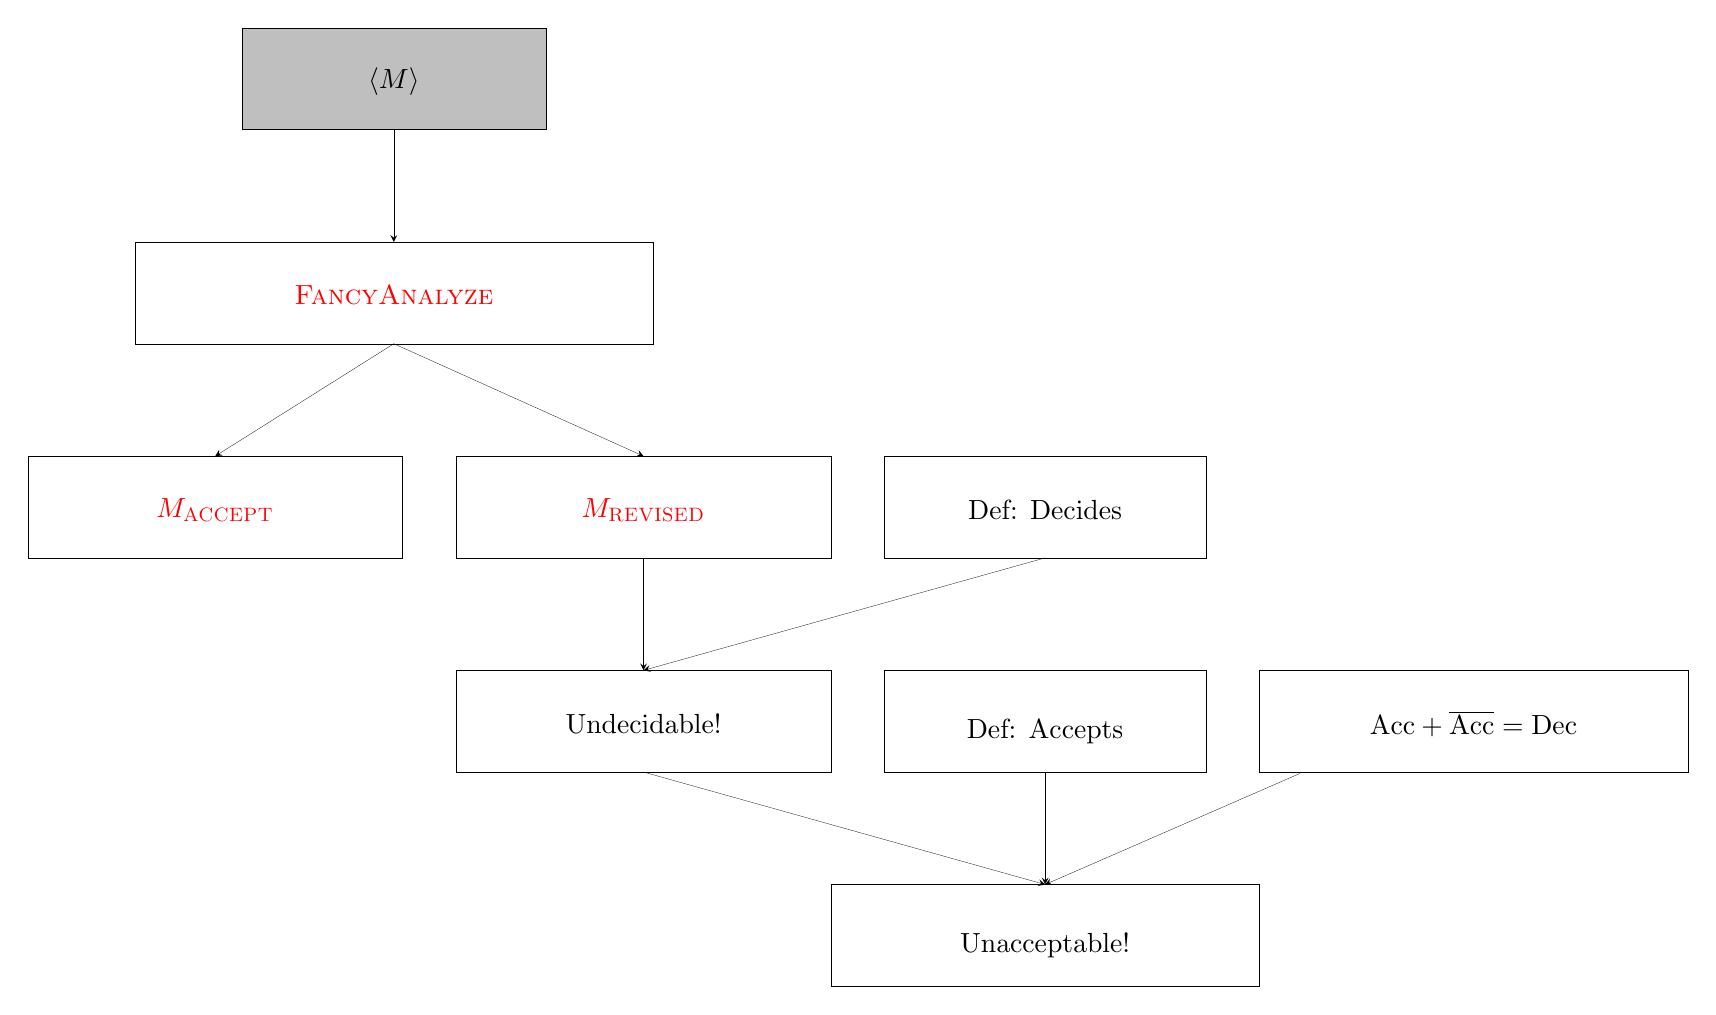
\begin{tikzpicture}
\pgftransformxscale{0.68000}
\pgftransformyscale{-0.680000}
\definecolor{dialinecolor}{rgb}{0.000000, 0.000000, 0.000000}
\pgfsetstrokecolor{dialinecolor}
\definecolor{dialinecolor}{rgb}{1.000000, 1.000000, 1.000000}
\pgfsetfillcolor{dialinecolor}
\definecolor{dialinecolor}{rgb}{1.000000, 1.000000, 1.000000}
\pgfsetfillcolor{dialinecolor}
\fill (12.000000\du,9.000000\du)--(12.000000\du,10.900000\du)--(19.000000\du,10.900000\du)--(19.000000\du,9.000000\du)--cycle;
\pgfsetlinewidth{0.100000\du}
\pgfsetdash{}{0pt}
\pgfsetdash{}{0pt}
\pgfsetmiterjoin
\definecolor{dialinecolor}{rgb}{0.000000, 0.000000, 0.000000}
\pgfsetstrokecolor{dialinecolor}
\draw (12.000000\du,9.000000\du)--(12.000000\du,10.900000\du)--(19.000000\du,10.900000\du)--(19.000000\du,9.000000\du)--cycle;
% setfont left to latex
\definecolor{dialinecolor}{rgb}{0.000000, 0.000000, 0.000000}
\pgfsetstrokecolor{dialinecolor}
\node at (15.500000\du,10.000\du){\MACC};
\definecolor{dialinecolor}{rgb}{1.000000, 1.000000, 1.000000}
\pgfsetfillcolor{dialinecolor}
\fill (20.000000\du,9.000000\du)--(20.000000\du,10.900000\du)--(27.000000\du,10.900000\du)--(27.000000\du,9.000000\du)--cycle;
\pgfsetlinewidth{0.100000\du}
\pgfsetdash{}{0pt}
\pgfsetdash{}{0pt}
\pgfsetmiterjoin
\definecolor{dialinecolor}{rgb}{0.000000, 0.000000, 0.000000}
\pgfsetstrokecolor{dialinecolor}
\draw (20.000000\du,9.000000\du)--(20.000000\du,10.900000\du)--(27.000000\du,10.900000\du)--(27.000000\du,9.000000\du)--cycle;
% setfont left to latex
\definecolor{dialinecolor}{rgb}{0.000000, 0.000000, 0.000000}
\pgfsetstrokecolor{dialinecolor}
\node at (23.500000\du,10.000\du){\MREV};
\definecolor{dialinecolor}{rgb}{1.000000, 1.000000, 1.000000}
\pgfsetfillcolor{dialinecolor}
\fill (35.000000\du,13.000000\du)--(35.000000\du,14.900000\du)--(41.000000\du,14.900000\du)--(41.000000\du,13.000000\du)--cycle;
\pgfsetlinewidth{0.100000\du}
\pgfsetdash{}{0pt}
\pgfsetdash{}{0pt}
\pgfsetmiterjoin
\definecolor{dialinecolor}{rgb}{0.000000, 0.000000, 0.000000}
\pgfsetstrokecolor{dialinecolor}
\draw (35.000000\du,13.000000\du)--(35.000000\du,14.900000\du)--(43.000000\du,14.900000\du)--(43.000000\du,13.000000\du)--cycle;
% setfont left to latex
\definecolor{dialinecolor}{rgb}{0.000000, 0.000000, 0.000000}
\pgfsetstrokecolor{dialinecolor}
\node at (39.000000\du,14.0000\du){$\text{Acc}+\overline{\text{Acc}}=\text{Dec}$};
\definecolor{dialinecolor}{rgb}{1.000000, 1.000000, 1.000000}
\pgfsetfillcolor{dialinecolor}
\fill (16.000000\du,5.000000\du)--(16.000000\du,6.900000\du)--(21.672500\du,6.900000\du)--(21.672500\du,5.000000\du)--cycle;
\pgfsetlinewidth{0.100000\du}
\pgfsetdash{}{0pt}
\pgfsetdash{}{0pt}
\pgfsetmiterjoin
\definecolor{dialinecolor}{rgb}{0.000000, 0.000000, 0.000000}
\pgfsetstrokecolor{dialinecolor}
\draw (14.000000\du,5.000000\du)--(14.000000\du,6.900000\du)--(23.672500\du,6.900000\du)--(23.672500\du,5.000000\du)--cycle;
% setfont left to latex
\definecolor{dialinecolor}{rgb}{0.000000, 0.000000, 0.000000}
\pgfsetstrokecolor{dialinecolor}
\node at (18.836250\du,6.000\du){\func{FancyAnalyze}};
\definecolor{dialinecolor}{rgb}{1.000000, 1.000000, 1.000000}
\pgfsetfillcolor{dialinecolor}
\fill (28.000000\du,13.000000\du)--(28.000000\du,14.900000\du)--(34.000000\du,14.900000\du)--(34.000000\du,13.000000\du)--cycle;
\pgfsetlinewidth{0.100000\du}
\pgfsetdash{}{0pt}
\pgfsetdash{}{0pt}
\pgfsetmiterjoin
\definecolor{dialinecolor}{rgb}{0.000000, 0.000000, 0.000000}
\pgfsetstrokecolor{dialinecolor}
\pgfsetfillcolor{black!25}
\fill (16.000000\du,1.000000\du)--(16.000000\du,2.900000\du)--(21.672500\du,2.900000\du)--(21.672500\du,1.000000\du)--cycle;
\definecolor{dialinecolor}{rgb}{0.000000, 0.000000, 0.000000}\draw (16.000000\du,1.000000\du)--(16.000000\du,2.900000\du)--(21.672500\du,2.900000\du)--(21.672500\du,1.000000\du)--cycle;
% setfont left to latex
\definecolor{dialinecolor}{rgb}{0.000000, 0.000000, 0.000000}
\pgfsetstrokecolor{dialinecolor}
\node at (18.836250\du,2.000\du){\str{M}};
\definecolor{dialinecolor}{rgb}{1.000000, 1.000000, 1.000000}
\pgfsetfillcolor{dialinecolor}
\fill (28.000000\du,13.000000\du)--(28.000000\du,14.900000\du)--(34.000000\du,14.900000\du)--(34.000000\du,13.000000\du)--cycle;
\pgfsetlinewidth{0.100000\du}
\pgfsetdash{}{0pt}
\pgfsetdash{}{0pt}
\pgfsetmiterjoin
\definecolor{dialinecolor}{rgb}{0.000000, 0.000000, 0.000000}
\pgfsetstrokecolor{dialinecolor}
\draw (28.000000\du,13.000000\du)--(28.000000\du,14.900000\du)--(34.000000\du,14.900000\du)--(34.000000\du,13.000000\du)--cycle;
% setfont left to latex
\definecolor{dialinecolor}{rgb}{0.000000, 0.000000, 0.000000}
\pgfsetstrokecolor{dialinecolor}
\node at (31.000000\du,14.145000\du){Def: Accepts};
\definecolor{dialinecolor}{rgb}{1.000000, 1.000000, 1.000000}
\pgfsetfillcolor{dialinecolor}
\fill (28.000000\du,9.000000\du)--(28.000000\du,10.900000\du)--(34.000000\du,10.900000\du)--(34.000000\du,9.000000\du)--cycle;
\pgfsetlinewidth{0.100000\du}
\pgfsetdash{}{0pt}
\pgfsetdash{}{0pt}
\pgfsetmiterjoin
\definecolor{dialinecolor}{rgb}{0.000000, 0.000000, 0.000000}
\pgfsetstrokecolor{dialinecolor}
\draw (28.000000\du,9.000000\du)--(28.000000\du,10.900000\du)--(34.000000\du,10.900000\du)--(34.000000\du,9.000000\du)--cycle;
% setfont left to latex
\definecolor{dialinecolor}{rgb}{0.000000, 0.000000, 0.000000}
\pgfsetstrokecolor{dialinecolor}
\node at (31.000000\du,10.000\du){Def: Decides};
\definecolor{dialinecolor}{rgb}{1.000000, 1.000000, 1.000000}
\pgfsetfillcolor{dialinecolor}
\fill (20.000000\du,13.000000\du)--(20.000000\du,14.900000\du)--(27.000000\du,14.900000\du)--(27.000000\du,13.000000\du)--cycle;
\pgfsetlinewidth{0.100000\du}
\pgfsetdash{}{0pt}
\pgfsetdash{}{0pt}
\pgfsetmiterjoin
\definecolor{dialinecolor}{rgb}{0.000000, 0.000000, 0.000000}
\pgfsetstrokecolor{dialinecolor}
\draw (20.000000\du,13.000000\du)--(20.000000\du,14.900000\du)--(27.000000\du,14.900000\du)--(27.000000\du,13.000000\du)--cycle;
% setfont left to latex
\definecolor{dialinecolor}{rgb}{0.000000, 0.000000, 0.000000}
\pgfsetstrokecolor{dialinecolor}
\node at (23.500000\du,14.000\du){Undecidable!};
\definecolor{dialinecolor}{rgb}{1.000000, 1.000000, 1.000000}
\pgfsetfillcolor{dialinecolor}
\fill (28.000000\du,17.000000\du)--(28.000000\du,18.900000\du)--(34.000000\du,18.900000\du)--(34.000000\du,17.000000\du)--cycle;
\pgfsetlinewidth{0.100000\du}
\pgfsetdash{}{0pt}
\pgfsetdash{}{0pt}
\pgfsetmiterjoin
\definecolor{dialinecolor}{rgb}{0.000000, 0.000000, 0.000000}
\pgfsetstrokecolor{dialinecolor}
\draw (27.000000\du,17.000000\du)--(27.000000\du,18.900000\du)--(35.000000\du,18.900000\du)--(35.000000\du,17.000000\du)--cycle;
% setfont left to latex
\definecolor{dialinecolor}{rgb}{0.000000, 0.000000, 0.000000}
\pgfsetstrokecolor{dialinecolor}
\node at (31.000000\du,18.145000\du){Unacceptable!};
\pgfsetlinewidth{0.100000\du}
\pgfsetdash{}{0pt}
\pgfsetdash{}{0pt}
\pgfsetbuttcap
{
\definecolor{dialinecolor}{rgb}{0.000000, 0.000000, 0.000000}
\pgfsetfillcolor{dialinecolor}
% was here!!!
\pgfsetarrowsend{stealth}
\definecolor{dialinecolor}{rgb}{0.000000, 0.000000, 0.000000}
\pgfsetstrokecolor{dialinecolor}
\draw (18.836250\du,2.900000\du)--(18.836250\du,5.000000\du);
}
\pgfsetlinewidth{0.100000\du}
\pgfsetdash{}{0pt}
\pgfsetdash{}{0pt}
\pgfsetbuttcap
{
\definecolor{dialinecolor}{rgb}{0.000000, 0.000000, 0.000000}
\pgfsetfillcolor{dialinecolor}
% was here!!!
\pgfsetarrowsend{stealth}
\definecolor{dialinecolor}{rgb}{0.000000, 0.000000, 0.000000}
\pgfsetstrokecolor{dialinecolor}
\draw (18.836250\du,6.900000\du)--(15.500000\du,9.000000\du);
}
\pgfsetlinewidth{0.100000\du}
\pgfsetdash{}{0pt}
\pgfsetdash{}{0pt}
\pgfsetbuttcap
{
\definecolor{dialinecolor}{rgb}{0.000000, 0.000000, 0.000000}
\pgfsetfillcolor{dialinecolor}
% was here!!!
\pgfsetarrowsend{stealth}
\definecolor{dialinecolor}{rgb}{0.000000, 0.000000, 0.000000}
\pgfsetstrokecolor{dialinecolor}
\draw (18.836250\du,6.900000\du)--(23.500000\du,9.000000\du);
}
\pgfsetlinewidth{0.100000\du}
\pgfsetdash{}{0pt}
\pgfsetdash{}{0pt}
\pgfsetbuttcap
{
\definecolor{dialinecolor}{rgb}{0.000000, 0.000000, 0.000000}
\pgfsetfillcolor{dialinecolor}
% was here!!!
\pgfsetarrowsend{stealth}
\definecolor{dialinecolor}{rgb}{0.000000, 0.000000, 0.000000}
\pgfsetstrokecolor{dialinecolor}
\draw (23.500000\du,10.900000\du)--(23.500000\du,13.000000\du);
}
\pgfsetlinewidth{0.100000\du}
\pgfsetdash{}{0pt}
\pgfsetdash{}{0pt}
\pgfsetbuttcap
{
\definecolor{dialinecolor}{rgb}{0.000000, 0.000000, 0.000000}
\pgfsetfillcolor{dialinecolor}
% was here!!!
\pgfsetarrowsend{stealth}
\definecolor{dialinecolor}{rgb}{0.000000, 0.000000, 0.000000}
\pgfsetstrokecolor{dialinecolor}
\draw (31.000000\du,10.900000\du)--(23.500000\du,13.000000\du);
}
\pgfsetlinewidth{0.100000\du}
\pgfsetdash{}{0pt}
\pgfsetdash{}{0pt}
\pgfsetbuttcap
{
\definecolor{dialinecolor}{rgb}{0.000000, 0.000000, 0.000000}
\pgfsetfillcolor{dialinecolor}
% was here!!!
\pgfsetarrowsend{stealth}
\definecolor{dialinecolor}{rgb}{0.000000, 0.000000, 0.000000}
\pgfsetstrokecolor{dialinecolor}
\draw (23.500000\du,14.900000\du)--(31.000000\du,17.000000\du);
}
\pgfsetlinewidth{0.100000\du}
\pgfsetdash{}{0pt}
\pgfsetdash{}{0pt}
\pgfsetbuttcap
{
\definecolor{dialinecolor}{rgb}{0.000000, 0.000000, 0.000000}
\pgfsetfillcolor{dialinecolor}
% was here!!!
\pgfsetarrowsend{stealth}
\definecolor{dialinecolor}{rgb}{0.000000, 0.000000, 0.000000}
\pgfsetstrokecolor{dialinecolor}
\draw (31.000000\du,14.900000\du)--(31.000000\du,17.000000\du);
}
\pgfsetlinewidth{0.100000\du}
\pgfsetdash{}{0pt}
\pgfsetdash{}{0pt}
\pgfsetbuttcap
{
\definecolor{dialinecolor}{rgb}{0.000000, 0.000000, 0.000000}
\pgfsetfillcolor{dialinecolor}
% was here!!!
\pgfsetarrowsend{stealth}
\definecolor{dialinecolor}{rgb}{0.000000, 0.000000, 0.000000}
\pgfsetstrokecolor{dialinecolor}
\draw (35.757813\du,14.926953\du)--(31.000000\du,17.000000\du);
}
\end{tikzpicture}
}

\end{frame}

\begin{frame}{A fancy analyzer of Turing Machines}

  Suppose we wrote a function, \func{FancyAnalyze}(\str{M},$w$), that could do the
  following:

  \begin{itemize}

  \item Analyze how $M$ (described by the string \str{M})
    behaves on input $w$. (Don't actually simulate $M$!)

  \item If $M$ \textit{accepts} $w$, then \func{FancyAnalyze} returns \textit{accept}.

  \item If $M$ \textit{rejects} $w$, then \func{FancyAnalyze} returns \textit{reject}.

  \item If $M$ can be shown to get stuck in a loop on $w$, and therefore
    never accepts or rejects, then \func{FancyAnalyze} returns \textit{loops}.

  \end{itemize}

  Could a fancy programmer write \func{FancyAnalyze} \dots ?

\end{frame}

\begin{frame}{The Plan}

  % Graphic for TeX using PGF
% Title: C:\Users\Joshua\Documents\teaching\csueb-guest-teaching\flow-diagram.dia
% Creator: Dia v0.97.2
% CreationDate: Tue Feb 04 08:43:25 2014
% For: Joshua
% \usepackage{tikz}
% The following commands are not supported in PSTricks at present
% We define them conditionally, so when they are implemented,
% this pgf file will use them.
\ifx\du\undefined
  \newlength{\du}
\fi
\setlength{\du}{15\unitlength}
{\footnotesize
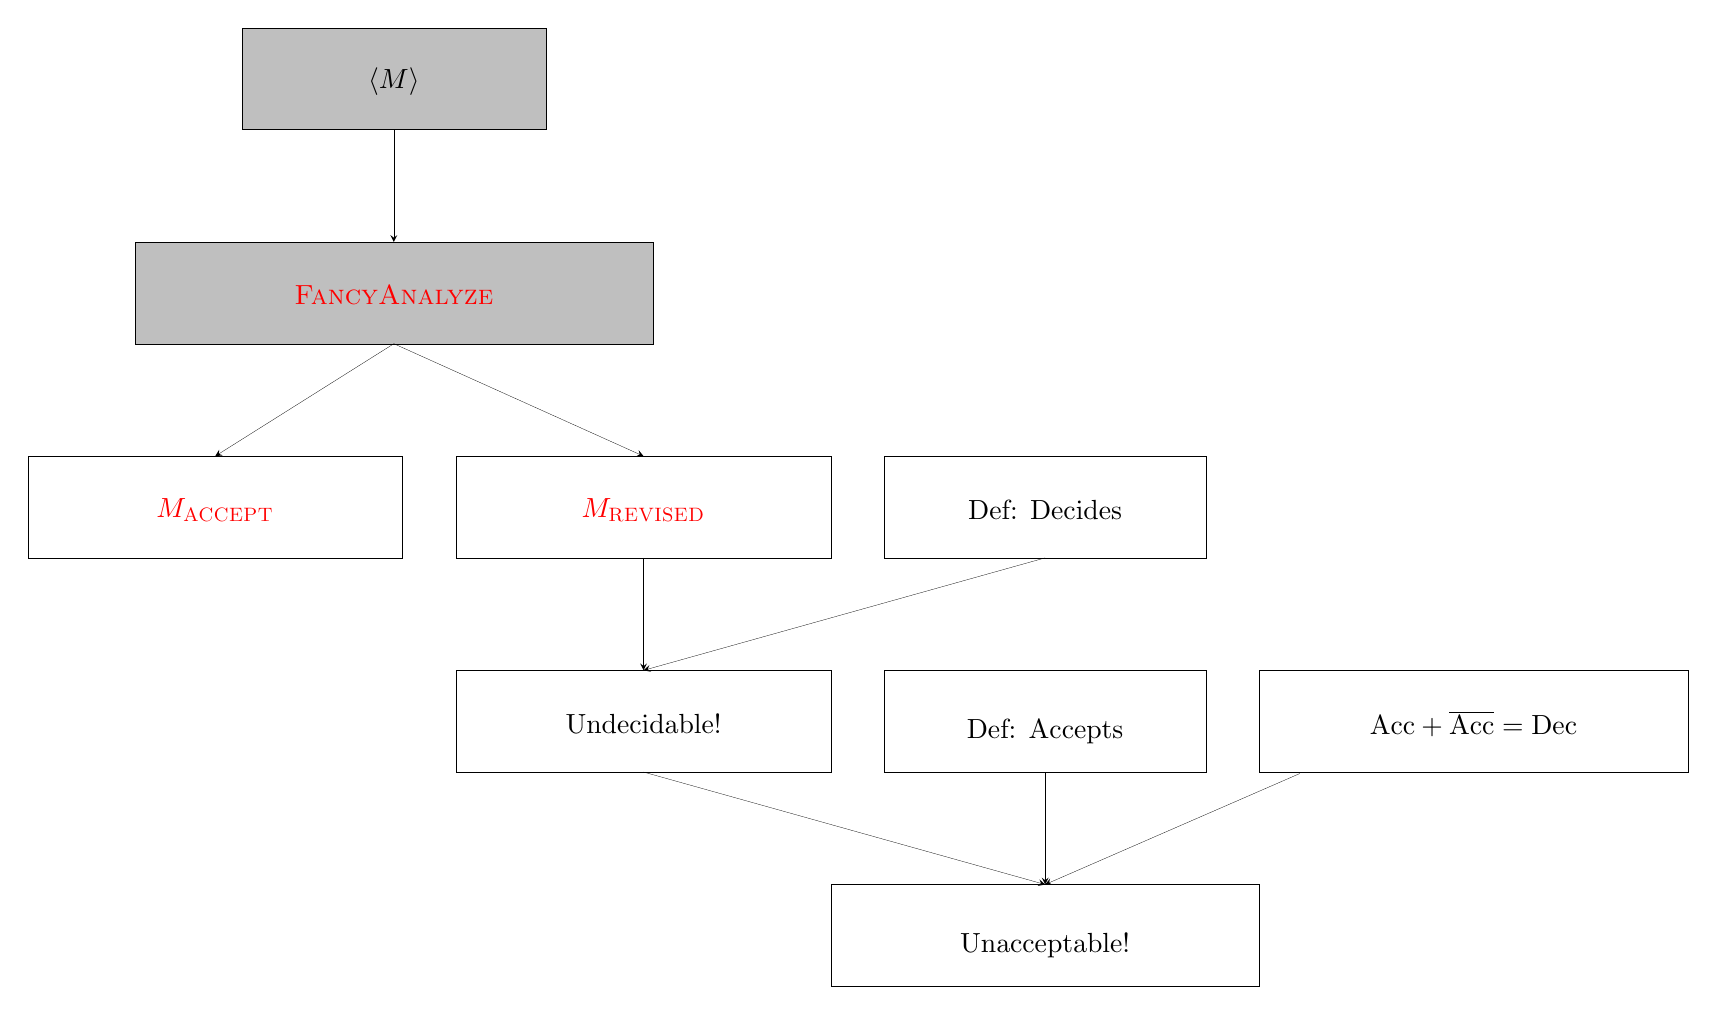
\begin{tikzpicture}
\pgftransformxscale{0.68000}
\pgftransformyscale{-0.680000}
\definecolor{dialinecolor}{rgb}{0.000000, 0.000000, 0.000000}
\pgfsetstrokecolor{dialinecolor}
\definecolor{dialinecolor}{rgb}{1.000000, 1.000000, 1.000000}
\pgfsetfillcolor{dialinecolor}
\definecolor{dialinecolor}{rgb}{1.000000, 1.000000, 1.000000}
\pgfsetfillcolor{dialinecolor}
\fill (12.000000\du,9.000000\du)--(12.000000\du,10.900000\du)--(19.000000\du,10.900000\du)--(19.000000\du,9.000000\du)--cycle;
\pgfsetlinewidth{0.100000\du}
\pgfsetdash{}{0pt}
\pgfsetdash{}{0pt}
\pgfsetmiterjoin
\definecolor{dialinecolor}{rgb}{0.000000, 0.000000, 0.000000}
\pgfsetstrokecolor{dialinecolor}
\draw (12.000000\du,9.000000\du)--(12.000000\du,10.900000\du)--(19.000000\du,10.900000\du)--(19.000000\du,9.000000\du)--cycle;
% setfont left to latex
\definecolor{dialinecolor}{rgb}{0.000000, 0.000000, 0.000000}
\pgfsetstrokecolor{dialinecolor}
\node at (15.500000\du,10.000\du){\MACC};
\definecolor{dialinecolor}{rgb}{1.000000, 1.000000, 1.000000}
\pgfsetfillcolor{dialinecolor}
\fill (20.000000\du,9.000000\du)--(20.000000\du,10.900000\du)--(27.000000\du,10.900000\du)--(27.000000\du,9.000000\du)--cycle;
\pgfsetlinewidth{0.100000\du}
\pgfsetdash{}{0pt}
\pgfsetdash{}{0pt}
\pgfsetmiterjoin
\definecolor{dialinecolor}{rgb}{0.000000, 0.000000, 0.000000}
\pgfsetstrokecolor{dialinecolor}
\draw (20.000000\du,9.000000\du)--(20.000000\du,10.900000\du)--(27.000000\du,10.900000\du)--(27.000000\du,9.000000\du)--cycle;
% setfont left to latex
\definecolor{dialinecolor}{rgb}{0.000000, 0.000000, 0.000000}
\pgfsetstrokecolor{dialinecolor}
\node at (23.500000\du,10.000\du){\MREV};
\definecolor{dialinecolor}{rgb}{1.000000, 1.000000, 1.000000}
\pgfsetfillcolor{dialinecolor}
\fill (35.000000\du,13.000000\du)--(35.000000\du,14.900000\du)--(41.000000\du,14.900000\du)--(41.000000\du,13.000000\du)--cycle;
\pgfsetlinewidth{0.100000\du}
\pgfsetdash{}{0pt}
\pgfsetdash{}{0pt}
\pgfsetmiterjoin
\definecolor{dialinecolor}{rgb}{0.000000, 0.000000, 0.000000}
\pgfsetstrokecolor{dialinecolor}
\draw (35.000000\du,13.000000\du)--(35.000000\du,14.900000\du)--(43.000000\du,14.900000\du)--(43.000000\du,13.000000\du)--cycle;
% setfont left to latex
\definecolor{dialinecolor}{rgb}{0.000000, 0.000000, 0.000000}
\pgfsetstrokecolor{dialinecolor}
\node at (39.000000\du,14.0000\du){$\text{Acc}+\overline{\text{Acc}}=\text{Dec}$};
\definecolor{dialinecolor}{rgb}{1.000000, 1.000000, 1.000000}
\pgfsetfillcolor{black!25}
\fill (14.000000\du,5.000000\du)--(14.000000\du,6.900000\du)--(23.672500\du,6.900000\du)--(23.672500\du,5.000000\du)--cycle;
\pgfsetlinewidth{0.100000\du}
\pgfsetdash{}{0pt}
\pgfsetdash{}{0pt}
\pgfsetmiterjoin
\definecolor{dialinecolor}{rgb}{0.000000, 0.000000, 0.000000}
\pgfsetstrokecolor{dialinecolor}
\draw (14.000000\du,5.000000\du)--(14.000000\du,6.900000\du)--(23.672500\du,6.900000\du)--(23.672500\du,5.000000\du)--cycle;
% setfont left to latex
\definecolor{dialinecolor}{rgb}{0.000000, 0.000000, 0.000000}
\pgfsetstrokecolor{dialinecolor}
\node at (18.836250\du,6.000\du){\func{FancyAnalyze}};
\definecolor{dialinecolor}{rgb}{1.000000, 1.000000, 1.000000}
\pgfsetfillcolor{dialinecolor}
\fill (28.000000\du,13.000000\du)--(28.000000\du,14.900000\du)--(34.000000\du,14.900000\du)--(34.000000\du,13.000000\du)--cycle;
\pgfsetlinewidth{0.100000\du}
\pgfsetdash{}{0pt}
\pgfsetdash{}{0pt}
\pgfsetmiterjoin
\definecolor{dialinecolor}{rgb}{0.000000, 0.000000, 0.000000}
\pgfsetstrokecolor{dialinecolor}
\pgfsetfillcolor{black!25}
\fill (16.000000\du,1.000000\du)--(16.000000\du,2.900000\du)--(21.672500\du,2.900000\du)--(21.672500\du,1.000000\du)--cycle;
\definecolor{dialinecolor}{rgb}{0.000000, 0.000000, 0.000000}\draw (16.000000\du,1.000000\du)--(16.000000\du,2.900000\du)--(21.672500\du,2.900000\du)--(21.672500\du,1.000000\du)--cycle;
% setfont left to latex
\definecolor{dialinecolor}{rgb}{0.000000, 0.000000, 0.000000}
\pgfsetstrokecolor{dialinecolor}
\node at (18.836250\du,2.000\du){\str{M}};
\definecolor{dialinecolor}{rgb}{1.000000, 1.000000, 1.000000}
\pgfsetfillcolor{dialinecolor}
\fill (28.000000\du,13.000000\du)--(28.000000\du,14.900000\du)--(34.000000\du,14.900000\du)--(34.000000\du,13.000000\du)--cycle;
\pgfsetlinewidth{0.100000\du}
\pgfsetdash{}{0pt}
\pgfsetdash{}{0pt}
\pgfsetmiterjoin
\definecolor{dialinecolor}{rgb}{0.000000, 0.000000, 0.000000}
\pgfsetstrokecolor{dialinecolor}
\draw (28.000000\du,13.000000\du)--(28.000000\du,14.900000\du)--(34.000000\du,14.900000\du)--(34.000000\du,13.000000\du)--cycle;
% setfont left to latex
\definecolor{dialinecolor}{rgb}{0.000000, 0.000000, 0.000000}
\pgfsetstrokecolor{dialinecolor}
\node at (31.000000\du,14.145000\du){Def: Accepts};
\definecolor{dialinecolor}{rgb}{1.000000, 1.000000, 1.000000}
\pgfsetfillcolor{dialinecolor}
\fill (28.000000\du,9.000000\du)--(28.000000\du,10.900000\du)--(34.000000\du,10.900000\du)--(34.000000\du,9.000000\du)--cycle;
\pgfsetlinewidth{0.100000\du}
\pgfsetdash{}{0pt}
\pgfsetdash{}{0pt}
\pgfsetmiterjoin
\definecolor{dialinecolor}{rgb}{0.000000, 0.000000, 0.000000}
\pgfsetstrokecolor{dialinecolor}
\draw (28.000000\du,9.000000\du)--(28.000000\du,10.900000\du)--(34.000000\du,10.900000\du)--(34.000000\du,9.000000\du)--cycle;
% setfont left to latex
\definecolor{dialinecolor}{rgb}{0.000000, 0.000000, 0.000000}
\pgfsetstrokecolor{dialinecolor}
\node at (31.000000\du,10.000\du){Def: Decides};
\definecolor{dialinecolor}{rgb}{1.000000, 1.000000, 1.000000}
\pgfsetfillcolor{dialinecolor}
\fill (20.000000\du,13.000000\du)--(20.000000\du,14.900000\du)--(27.000000\du,14.900000\du)--(27.000000\du,13.000000\du)--cycle;
\pgfsetlinewidth{0.100000\du}
\pgfsetdash{}{0pt}
\pgfsetdash{}{0pt}
\pgfsetmiterjoin
\definecolor{dialinecolor}{rgb}{0.000000, 0.000000, 0.000000}
\pgfsetstrokecolor{dialinecolor}
\draw (20.000000\du,13.000000\du)--(20.000000\du,14.900000\du)--(27.000000\du,14.900000\du)--(27.000000\du,13.000000\du)--cycle;
% setfont left to latex
\definecolor{dialinecolor}{rgb}{0.000000, 0.000000, 0.000000}
\pgfsetstrokecolor{dialinecolor}
\node at (23.500000\du,14.000\du){Undecidable!};
\definecolor{dialinecolor}{rgb}{1.000000, 1.000000, 1.000000}
\pgfsetfillcolor{dialinecolor}
\fill (28.000000\du,17.000000\du)--(28.000000\du,18.900000\du)--(34.000000\du,18.900000\du)--(34.000000\du,17.000000\du)--cycle;
\pgfsetlinewidth{0.100000\du}
\pgfsetdash{}{0pt}
\pgfsetdash{}{0pt}
\pgfsetmiterjoin
\definecolor{dialinecolor}{rgb}{0.000000, 0.000000, 0.000000}
\pgfsetstrokecolor{dialinecolor}
\draw (27.000000\du,17.000000\du)--(27.000000\du,18.900000\du)--(35.000000\du,18.900000\du)--(35.000000\du,17.000000\du)--cycle;
% setfont left to latex
\definecolor{dialinecolor}{rgb}{0.000000, 0.000000, 0.000000}
\pgfsetstrokecolor{dialinecolor}
\node at (31.000000\du,18.145000\du){Unacceptable!};
\pgfsetlinewidth{0.100000\du}
\pgfsetdash{}{0pt}
\pgfsetdash{}{0pt}
\pgfsetbuttcap
{
\definecolor{dialinecolor}{rgb}{0.000000, 0.000000, 0.000000}
\pgfsetfillcolor{dialinecolor}
% was here!!!
\pgfsetarrowsend{stealth}
\definecolor{dialinecolor}{rgb}{0.000000, 0.000000, 0.000000}
\pgfsetstrokecolor{dialinecolor}
\draw (18.836250\du,2.900000\du)--(18.836250\du,5.000000\du);
}
\pgfsetlinewidth{0.100000\du}
\pgfsetdash{}{0pt}
\pgfsetdash{}{0pt}
\pgfsetbuttcap
{
\definecolor{dialinecolor}{rgb}{0.000000, 0.000000, 0.000000}
\pgfsetfillcolor{dialinecolor}
% was here!!!
\pgfsetarrowsend{stealth}
\definecolor{dialinecolor}{rgb}{0.000000, 0.000000, 0.000000}
\pgfsetstrokecolor{dialinecolor}
\draw (18.836250\du,6.900000\du)--(15.500000\du,9.000000\du);
}
\pgfsetlinewidth{0.100000\du}
\pgfsetdash{}{0pt}
\pgfsetdash{}{0pt}
\pgfsetbuttcap
{
\definecolor{dialinecolor}{rgb}{0.000000, 0.000000, 0.000000}
\pgfsetfillcolor{dialinecolor}
% was here!!!
\pgfsetarrowsend{stealth}
\definecolor{dialinecolor}{rgb}{0.000000, 0.000000, 0.000000}
\pgfsetstrokecolor{dialinecolor}
\draw (18.836250\du,6.900000\du)--(23.500000\du,9.000000\du);
}
\pgfsetlinewidth{0.100000\du}
\pgfsetdash{}{0pt}
\pgfsetdash{}{0pt}
\pgfsetbuttcap
{
\definecolor{dialinecolor}{rgb}{0.000000, 0.000000, 0.000000}
\pgfsetfillcolor{dialinecolor}
% was here!!!
\pgfsetarrowsend{stealth}
\definecolor{dialinecolor}{rgb}{0.000000, 0.000000, 0.000000}
\pgfsetstrokecolor{dialinecolor}
\draw (23.500000\du,10.900000\du)--(23.500000\du,13.000000\du);
}
\pgfsetlinewidth{0.100000\du}
\pgfsetdash{}{0pt}
\pgfsetdash{}{0pt}
\pgfsetbuttcap
{
\definecolor{dialinecolor}{rgb}{0.000000, 0.000000, 0.000000}
\pgfsetfillcolor{dialinecolor}
% was here!!!
\pgfsetarrowsend{stealth}
\definecolor{dialinecolor}{rgb}{0.000000, 0.000000, 0.000000}
\pgfsetstrokecolor{dialinecolor}
\draw (31.000000\du,10.900000\du)--(23.500000\du,13.000000\du);
}
\pgfsetlinewidth{0.100000\du}
\pgfsetdash{}{0pt}
\pgfsetdash{}{0pt}
\pgfsetbuttcap
{
\definecolor{dialinecolor}{rgb}{0.000000, 0.000000, 0.000000}
\pgfsetfillcolor{dialinecolor}
% was here!!!
\pgfsetarrowsend{stealth}
\definecolor{dialinecolor}{rgb}{0.000000, 0.000000, 0.000000}
\pgfsetstrokecolor{dialinecolor}
\draw (23.500000\du,14.900000\du)--(31.000000\du,17.000000\du);
}
\pgfsetlinewidth{0.100000\du}
\pgfsetdash{}{0pt}
\pgfsetdash{}{0pt}
\pgfsetbuttcap
{
\definecolor{dialinecolor}{rgb}{0.000000, 0.000000, 0.000000}
\pgfsetfillcolor{dialinecolor}
% was here!!!
\pgfsetarrowsend{stealth}
\definecolor{dialinecolor}{rgb}{0.000000, 0.000000, 0.000000}
\pgfsetstrokecolor{dialinecolor}
\draw (31.000000\du,14.900000\du)--(31.000000\du,17.000000\du);
}
\pgfsetlinewidth{0.100000\du}
\pgfsetdash{}{0pt}
\pgfsetdash{}{0pt}
\pgfsetbuttcap
{
\definecolor{dialinecolor}{rgb}{0.000000, 0.000000, 0.000000}
\pgfsetfillcolor{dialinecolor}
% was here!!!
\pgfsetarrowsend{stealth}
\definecolor{dialinecolor}{rgb}{0.000000, 0.000000, 0.000000}
\pgfsetstrokecolor{dialinecolor}
\draw (35.757813\du,14.926953\du)--(31.000000\du,17.000000\du);
}
\end{tikzpicture}
}

\end{frame}

\begin{frame}{Using \func{FancyAnalyze} to create a self-decider}

  \MACC~identifies (decides) the class of ``machines
  that accept their own description.''

  \vskip 0.25in

  \begin{algorithmic}[0]
    \Function{\func{\MACC}}{\str{M}}

    \State Answer $\gets$ \func{FancyAnalyze}(\str{M}, \str{M})

    \If{Answer $=$ \textit{accept}}

    \Return \textit{accept}

    \ElsIf{Answer $=$ \textit{reject} or Answer $=$ \textit{loops}}

    \Return \textit{reject}

    \EndIf

    \EndFunction
    
  \end{algorithmic}

\end{frame}

\begin{frame}{A quick self-check}

  What does \MACC~do on input \strMACC?

  \vskip 0.25in

  \MACC(\strMACC) $=$

  \begin{itemize}

  \item If \func{FancyAnalyze}(\str{\MACC}, \str{\MACC}) returns \textit{accept}, then
    \MACC(\strMACC) returns \textit{accept}.

  \item If \func{FancyAnalyze}(\strMACC, \strMACC) returns \textit{reject} or \st{\textit{loop}},
    then \MACC(\strMACC) returns \textit{reject}.

  \end{itemize}

  Note: \func{FancyAnalyze}(\strMACC, \strMACC) won't return \textit{loop}
  because \MACC~is a decider.

\end{frame}

\begin{frame}{A quick self-check (in other words)}

  What does \MACC~do on input \strMACC?

  \vskip 0.25in

  \MACC(\strMACC) $=$

  \begin{itemize}

  \item If \MACC~accepts its own description, then it
    accepts its own description (duh).

  \item If \MACC~rejects its own description, then it
    rejects its own description (duh).

  \end{itemize}

\end{frame}

\begin{frame}{The Plan}

  % Graphic for TeX using PGF
% Title: C:\Users\Joshua\Documents\teaching\csueb-guest-teaching\flow-diagram.dia
% Creator: Dia v0.97.2
% CreationDate: Tue Feb 04 08:43:25 2014
% For: Joshua
% \usepackage{tikz}
% The following commands are not supported in PSTricks at present
% We define them conditionally, so when they are implemented,
% this pgf file will use them.
\ifx\du\undefined
  \newlength{\du}
\fi
\setlength{\du}{15\unitlength}
{\footnotesize
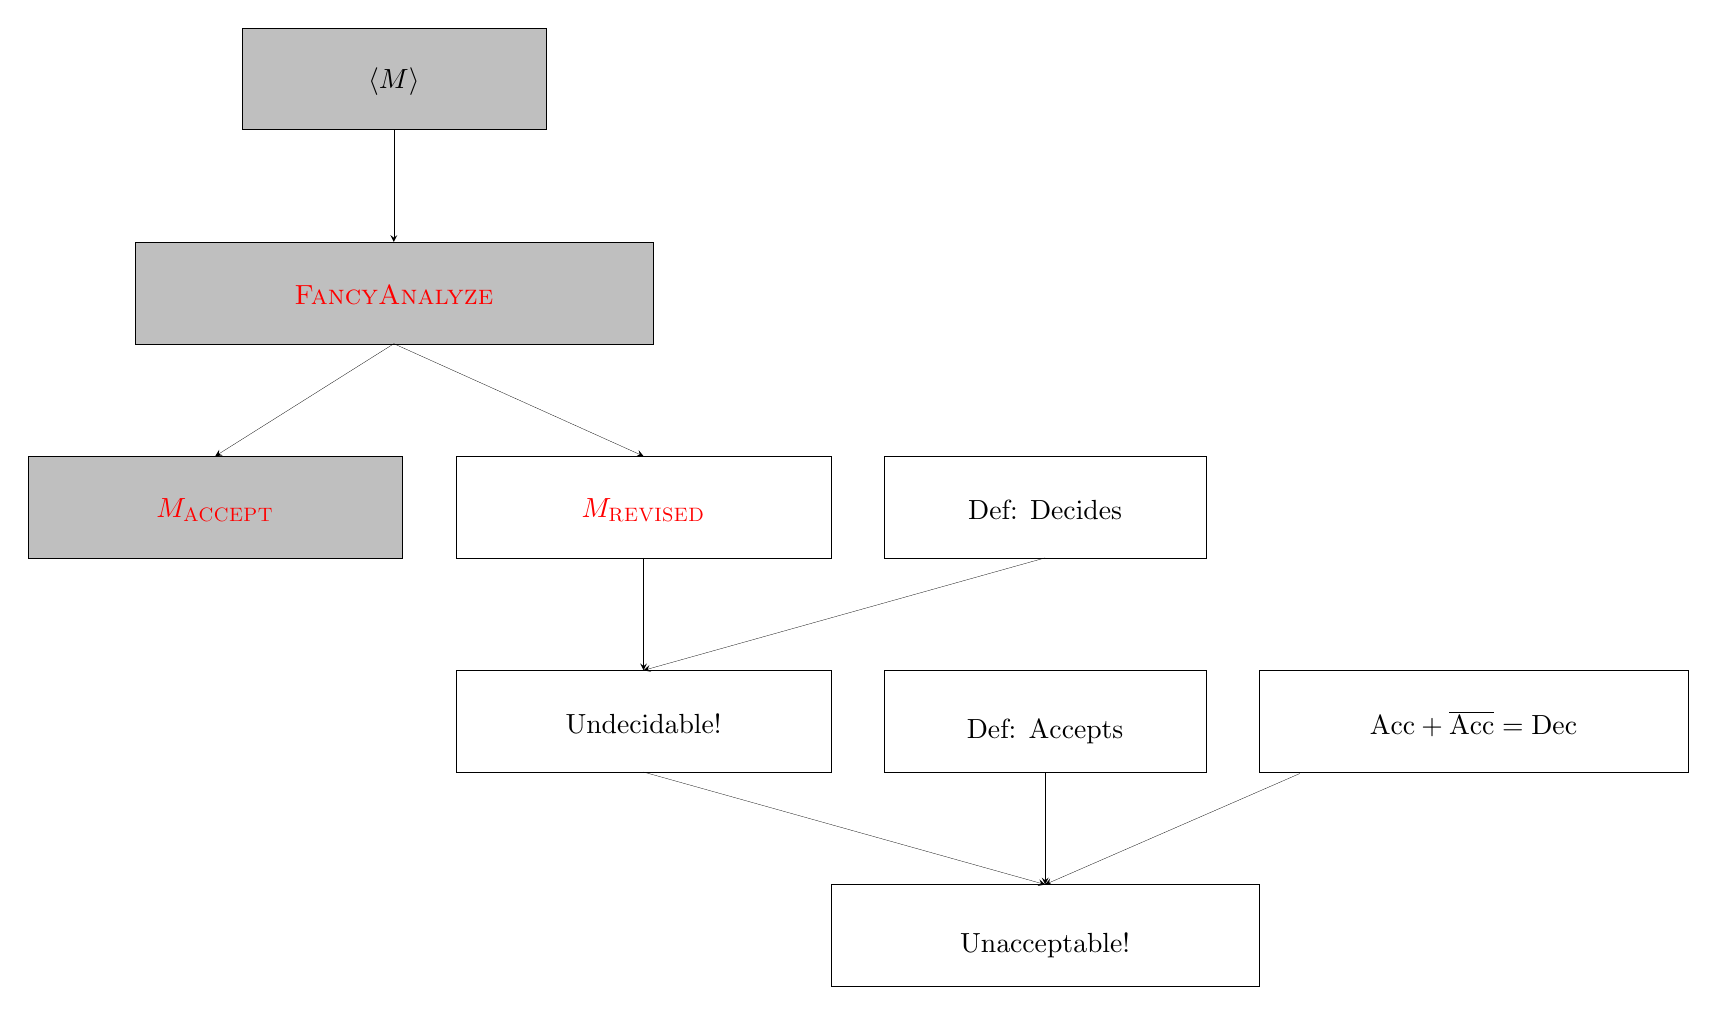
\begin{tikzpicture}
\pgftransformxscale{0.68000}
\pgftransformyscale{-0.680000}
\definecolor{dialinecolor}{rgb}{0.000000, 0.000000, 0.000000}
\pgfsetstrokecolor{dialinecolor}
\definecolor{dialinecolor}{rgb}{1.000000, 1.000000, 1.000000}
\pgfsetfillcolor{dialinecolor}
\definecolor{dialinecolor}{rgb}{1.000000, 1.000000, 1.000000}
\pgfsetfillcolor{black!25}
\fill (12.000000\du,9.000000\du)--(12.000000\du,10.900000\du)--(19.000000\du,10.900000\du)--(19.000000\du,9.000000\du)--cycle;
\pgfsetlinewidth{0.100000\du}
\pgfsetdash{}{0pt}
\pgfsetdash{}{0pt}
\pgfsetmiterjoin
\definecolor{dialinecolor}{rgb}{0.000000, 0.000000, 0.000000}
\pgfsetstrokecolor{dialinecolor}
\draw (12.000000\du,9.000000\du)--(12.000000\du,10.900000\du)--(19.000000\du,10.900000\du)--(19.000000\du,9.000000\du)--cycle;
% setfont left to latex
\definecolor{dialinecolor}{rgb}{0.000000, 0.000000, 0.000000}
\pgfsetstrokecolor{dialinecolor}
\node at (15.500000\du,10.000\du){\MACC};
\definecolor{dialinecolor}{rgb}{1.000000, 1.000000, 1.000000}
\pgfsetfillcolor{dialinecolor}
\fill (20.000000\du,9.000000\du)--(20.000000\du,10.900000\du)--(27.000000\du,10.900000\du)--(27.000000\du,9.000000\du)--cycle;
\pgfsetlinewidth{0.100000\du}
\pgfsetdash{}{0pt}
\pgfsetdash{}{0pt}
\pgfsetmiterjoin
\definecolor{dialinecolor}{rgb}{0.000000, 0.000000, 0.000000}
\pgfsetstrokecolor{dialinecolor}
\draw (20.000000\du,9.000000\du)--(20.000000\du,10.900000\du)--(27.000000\du,10.900000\du)--(27.000000\du,9.000000\du)--cycle;
% setfont left to latex
\definecolor{dialinecolor}{rgb}{0.000000, 0.000000, 0.000000}
\pgfsetstrokecolor{dialinecolor}
\node at (23.500000\du,10.000\du){\MREV};
\definecolor{dialinecolor}{rgb}{1.000000, 1.000000, 1.000000}
\pgfsetfillcolor{dialinecolor}
\fill (35.000000\du,13.000000\du)--(35.000000\du,14.900000\du)--(41.000000\du,14.900000\du)--(41.000000\du,13.000000\du)--cycle;
\pgfsetlinewidth{0.100000\du}
\pgfsetdash{}{0pt}
\pgfsetdash{}{0pt}
\pgfsetmiterjoin
\definecolor{dialinecolor}{rgb}{0.000000, 0.000000, 0.000000}
\pgfsetstrokecolor{dialinecolor}
\draw (35.000000\du,13.000000\du)--(35.000000\du,14.900000\du)--(43.000000\du,14.900000\du)--(43.000000\du,13.000000\du)--cycle;
% setfont left to latex
\definecolor{dialinecolor}{rgb}{0.000000, 0.000000, 0.000000}
\pgfsetstrokecolor{dialinecolor}
\node at (39.000000\du,14.0000\du){$\text{Acc}+\overline{\text{Acc}}=\text{Dec}$};
\definecolor{dialinecolor}{rgb}{1.000000, 1.000000, 1.000000}
\pgfsetfillcolor{black!25}
\fill (14.000000\du,5.000000\du)--(14.000000\du,6.900000\du)--(23.672500\du,6.900000\du)--(23.672500\du,5.000000\du)--cycle;
\pgfsetlinewidth{0.100000\du}
\pgfsetdash{}{0pt}
\pgfsetdash{}{0pt}
\pgfsetmiterjoin
\definecolor{dialinecolor}{rgb}{0.000000, 0.000000, 0.000000}
\pgfsetstrokecolor{dialinecolor}
\draw (14.000000\du,5.000000\du)--(14.000000\du,6.900000\du)--(23.672500\du,6.900000\du)--(23.672500\du,5.000000\du)--cycle;
% setfont left to latex
\definecolor{dialinecolor}{rgb}{0.000000, 0.000000, 0.000000}
\pgfsetstrokecolor{dialinecolor}
\node at (18.836250\du,6.000\du){\func{FancyAnalyze}};
\definecolor{dialinecolor}{rgb}{1.000000, 1.000000, 1.000000}
\pgfsetfillcolor{dialinecolor}
\fill (28.000000\du,13.000000\du)--(28.000000\du,14.900000\du)--(34.000000\du,14.900000\du)--(34.000000\du,13.000000\du)--cycle;
\pgfsetlinewidth{0.100000\du}
\pgfsetdash{}{0pt}
\pgfsetdash{}{0pt}
\pgfsetmiterjoin
\definecolor{dialinecolor}{rgb}{0.000000, 0.000000, 0.000000}
\pgfsetstrokecolor{dialinecolor}
\pgfsetfillcolor{black!25}
\fill (16.000000\du,1.000000\du)--(16.000000\du,2.900000\du)--(21.672500\du,2.900000\du)--(21.672500\du,1.000000\du)--cycle;
\definecolor{dialinecolor}{rgb}{0.000000, 0.000000, 0.000000}\draw (16.000000\du,1.000000\du)--(16.000000\du,2.900000\du)--(21.672500\du,2.900000\du)--(21.672500\du,1.000000\du)--cycle;
% setfont left to latex
\definecolor{dialinecolor}{rgb}{0.000000, 0.000000, 0.000000}
\pgfsetstrokecolor{dialinecolor}
\node at (18.836250\du,2.000\du){\str{M}};
\definecolor{dialinecolor}{rgb}{1.000000, 1.000000, 1.000000}
\pgfsetfillcolor{dialinecolor}
\fill (28.000000\du,13.000000\du)--(28.000000\du,14.900000\du)--(34.000000\du,14.900000\du)--(34.000000\du,13.000000\du)--cycle;
\pgfsetlinewidth{0.100000\du}
\pgfsetdash{}{0pt}
\pgfsetdash{}{0pt}
\pgfsetmiterjoin
\definecolor{dialinecolor}{rgb}{0.000000, 0.000000, 0.000000}
\pgfsetstrokecolor{dialinecolor}
\draw (28.000000\du,13.000000\du)--(28.000000\du,14.900000\du)--(34.000000\du,14.900000\du)--(34.000000\du,13.000000\du)--cycle;
% setfont left to latex
\definecolor{dialinecolor}{rgb}{0.000000, 0.000000, 0.000000}
\pgfsetstrokecolor{dialinecolor}
\node at (31.000000\du,14.145000\du){Def: Accepts};
\definecolor{dialinecolor}{rgb}{1.000000, 1.000000, 1.000000}
\pgfsetfillcolor{dialinecolor}
\fill (28.000000\du,9.000000\du)--(28.000000\du,10.900000\du)--(34.000000\du,10.900000\du)--(34.000000\du,9.000000\du)--cycle;
\pgfsetlinewidth{0.100000\du}
\pgfsetdash{}{0pt}
\pgfsetdash{}{0pt}
\pgfsetmiterjoin
\definecolor{dialinecolor}{rgb}{0.000000, 0.000000, 0.000000}
\pgfsetstrokecolor{dialinecolor}
\draw (28.000000\du,9.000000\du)--(28.000000\du,10.900000\du)--(34.000000\du,10.900000\du)--(34.000000\du,9.000000\du)--cycle;
% setfont left to latex
\definecolor{dialinecolor}{rgb}{0.000000, 0.000000, 0.000000}
\pgfsetstrokecolor{dialinecolor}
\node at (31.000000\du,10.000\du){Def: Decides};
\definecolor{dialinecolor}{rgb}{1.000000, 1.000000, 1.000000}
\pgfsetfillcolor{dialinecolor}
\fill (20.000000\du,13.000000\du)--(20.000000\du,14.900000\du)--(27.000000\du,14.900000\du)--(27.000000\du,13.000000\du)--cycle;
\pgfsetlinewidth{0.100000\du}
\pgfsetdash{}{0pt}
\pgfsetdash{}{0pt}
\pgfsetmiterjoin
\definecolor{dialinecolor}{rgb}{0.000000, 0.000000, 0.000000}
\pgfsetstrokecolor{dialinecolor}
\draw (20.000000\du,13.000000\du)--(20.000000\du,14.900000\du)--(27.000000\du,14.900000\du)--(27.000000\du,13.000000\du)--cycle;
% setfont left to latex
\definecolor{dialinecolor}{rgb}{0.000000, 0.000000, 0.000000}
\pgfsetstrokecolor{dialinecolor}
\node at (23.500000\du,14.000\du){Undecidable!};
\definecolor{dialinecolor}{rgb}{1.000000, 1.000000, 1.000000}
\pgfsetfillcolor{dialinecolor}
\fill (28.000000\du,17.000000\du)--(28.000000\du,18.900000\du)--(34.000000\du,18.900000\du)--(34.000000\du,17.000000\du)--cycle;
\pgfsetlinewidth{0.100000\du}
\pgfsetdash{}{0pt}
\pgfsetdash{}{0pt}
\pgfsetmiterjoin
\definecolor{dialinecolor}{rgb}{0.000000, 0.000000, 0.000000}
\pgfsetstrokecolor{dialinecolor}
\draw (27.000000\du,17.000000\du)--(27.000000\du,18.900000\du)--(35.000000\du,18.900000\du)--(35.000000\du,17.000000\du)--cycle;
% setfont left to latex
\definecolor{dialinecolor}{rgb}{0.000000, 0.000000, 0.000000}
\pgfsetstrokecolor{dialinecolor}
\node at (31.000000\du,18.145000\du){Unacceptable!};
\pgfsetlinewidth{0.100000\du}
\pgfsetdash{}{0pt}
\pgfsetdash{}{0pt}
\pgfsetbuttcap
{
\definecolor{dialinecolor}{rgb}{0.000000, 0.000000, 0.000000}
\pgfsetfillcolor{dialinecolor}
% was here!!!
\pgfsetarrowsend{stealth}
\definecolor{dialinecolor}{rgb}{0.000000, 0.000000, 0.000000}
\pgfsetstrokecolor{dialinecolor}
\draw (18.836250\du,2.900000\du)--(18.836250\du,5.000000\du);
}
\pgfsetlinewidth{0.100000\du}
\pgfsetdash{}{0pt}
\pgfsetdash{}{0pt}
\pgfsetbuttcap
{
\definecolor{dialinecolor}{rgb}{0.000000, 0.000000, 0.000000}
\pgfsetfillcolor{dialinecolor}
% was here!!!
\pgfsetarrowsend{stealth}
\definecolor{dialinecolor}{rgb}{0.000000, 0.000000, 0.000000}
\pgfsetstrokecolor{dialinecolor}
\draw (18.836250\du,6.900000\du)--(15.500000\du,9.000000\du);
}
\pgfsetlinewidth{0.100000\du}
\pgfsetdash{}{0pt}
\pgfsetdash{}{0pt}
\pgfsetbuttcap
{
\definecolor{dialinecolor}{rgb}{0.000000, 0.000000, 0.000000}
\pgfsetfillcolor{dialinecolor}
% was here!!!
\pgfsetarrowsend{stealth}
\definecolor{dialinecolor}{rgb}{0.000000, 0.000000, 0.000000}
\pgfsetstrokecolor{dialinecolor}
\draw (18.836250\du,6.900000\du)--(23.500000\du,9.000000\du);
}
\pgfsetlinewidth{0.100000\du}
\pgfsetdash{}{0pt}
\pgfsetdash{}{0pt}
\pgfsetbuttcap
{
\definecolor{dialinecolor}{rgb}{0.000000, 0.000000, 0.000000}
\pgfsetfillcolor{dialinecolor}
% was here!!!
\pgfsetarrowsend{stealth}
\definecolor{dialinecolor}{rgb}{0.000000, 0.000000, 0.000000}
\pgfsetstrokecolor{dialinecolor}
\draw (23.500000\du,10.900000\du)--(23.500000\du,13.000000\du);
}
\pgfsetlinewidth{0.100000\du}
\pgfsetdash{}{0pt}
\pgfsetdash{}{0pt}
\pgfsetbuttcap
{
\definecolor{dialinecolor}{rgb}{0.000000, 0.000000, 0.000000}
\pgfsetfillcolor{dialinecolor}
% was here!!!
\pgfsetarrowsend{stealth}
\definecolor{dialinecolor}{rgb}{0.000000, 0.000000, 0.000000}
\pgfsetstrokecolor{dialinecolor}
\draw (31.000000\du,10.900000\du)--(23.500000\du,13.000000\du);
}
\pgfsetlinewidth{0.100000\du}
\pgfsetdash{}{0pt}
\pgfsetdash{}{0pt}
\pgfsetbuttcap
{
\definecolor{dialinecolor}{rgb}{0.000000, 0.000000, 0.000000}
\pgfsetfillcolor{dialinecolor}
% was here!!!
\pgfsetarrowsend{stealth}
\definecolor{dialinecolor}{rgb}{0.000000, 0.000000, 0.000000}
\pgfsetstrokecolor{dialinecolor}
\draw (23.500000\du,14.900000\du)--(31.000000\du,17.000000\du);
}
\pgfsetlinewidth{0.100000\du}
\pgfsetdash{}{0pt}
\pgfsetdash{}{0pt}
\pgfsetbuttcap
{
\definecolor{dialinecolor}{rgb}{0.000000, 0.000000, 0.000000}
\pgfsetfillcolor{dialinecolor}
% was here!!!
\pgfsetarrowsend{stealth}
\definecolor{dialinecolor}{rgb}{0.000000, 0.000000, 0.000000}
\pgfsetstrokecolor{dialinecolor}
\draw (31.000000\du,14.900000\du)--(31.000000\du,17.000000\du);
}
\pgfsetlinewidth{0.100000\du}
\pgfsetdash{}{0pt}
\pgfsetdash{}{0pt}
\pgfsetbuttcap
{
\definecolor{dialinecolor}{rgb}{0.000000, 0.000000, 0.000000}
\pgfsetfillcolor{dialinecolor}
% was here!!!
\pgfsetarrowsend{stealth}
\definecolor{dialinecolor}{rgb}{0.000000, 0.000000, 0.000000}
\pgfsetstrokecolor{dialinecolor}
\draw (35.757813\du,14.926953\du)--(31.000000\du,17.000000\du);
}
\end{tikzpicture}
}

\end{frame}

\begin{frame}{A backwards self-decider (why not?)}

  \begin{algorithmic}[0]
    \Function{\MREV}{\str{M}}

    \State Answer $\gets$ \func{FancyAnalyze}(\str{M}, \str{M})

    \If{Answer $=$ \textit{accept}}

    \Return \textit{reject} \Comment{\textcolor{blue}{opposite!}}

    \ElsIf{Answer $=$ \textit{reject} or Answer $=$ \textit{loops}}

    \Return \textit{accept} \Comment{\textcolor{blue}{opposite!}}

    \EndIf

    \EndFunction
    
  \end{algorithmic}

  If you believe that we could implement \MACC, then you
  have to allow us to implement \MREV.

\end{frame}

\begin{frame}{The Plan}

  % Graphic for TeX using PGF
% Title: C:\Users\Joshua\Documents\teaching\csueb-guest-teaching\flow-diagram.dia
% Creator: Dia v0.97.2
% CreationDate: Tue Feb 04 08:43:25 2014
% For: Joshua
% \usepackage{tikz}
% The following commands are not supported in PSTricks at present
% We define them conditionally, so when they are implemented,
% this pgf file will use them.
\ifx\du\undefined
  \newlength{\du}
\fi
\setlength{\du}{15\unitlength}
{\footnotesize
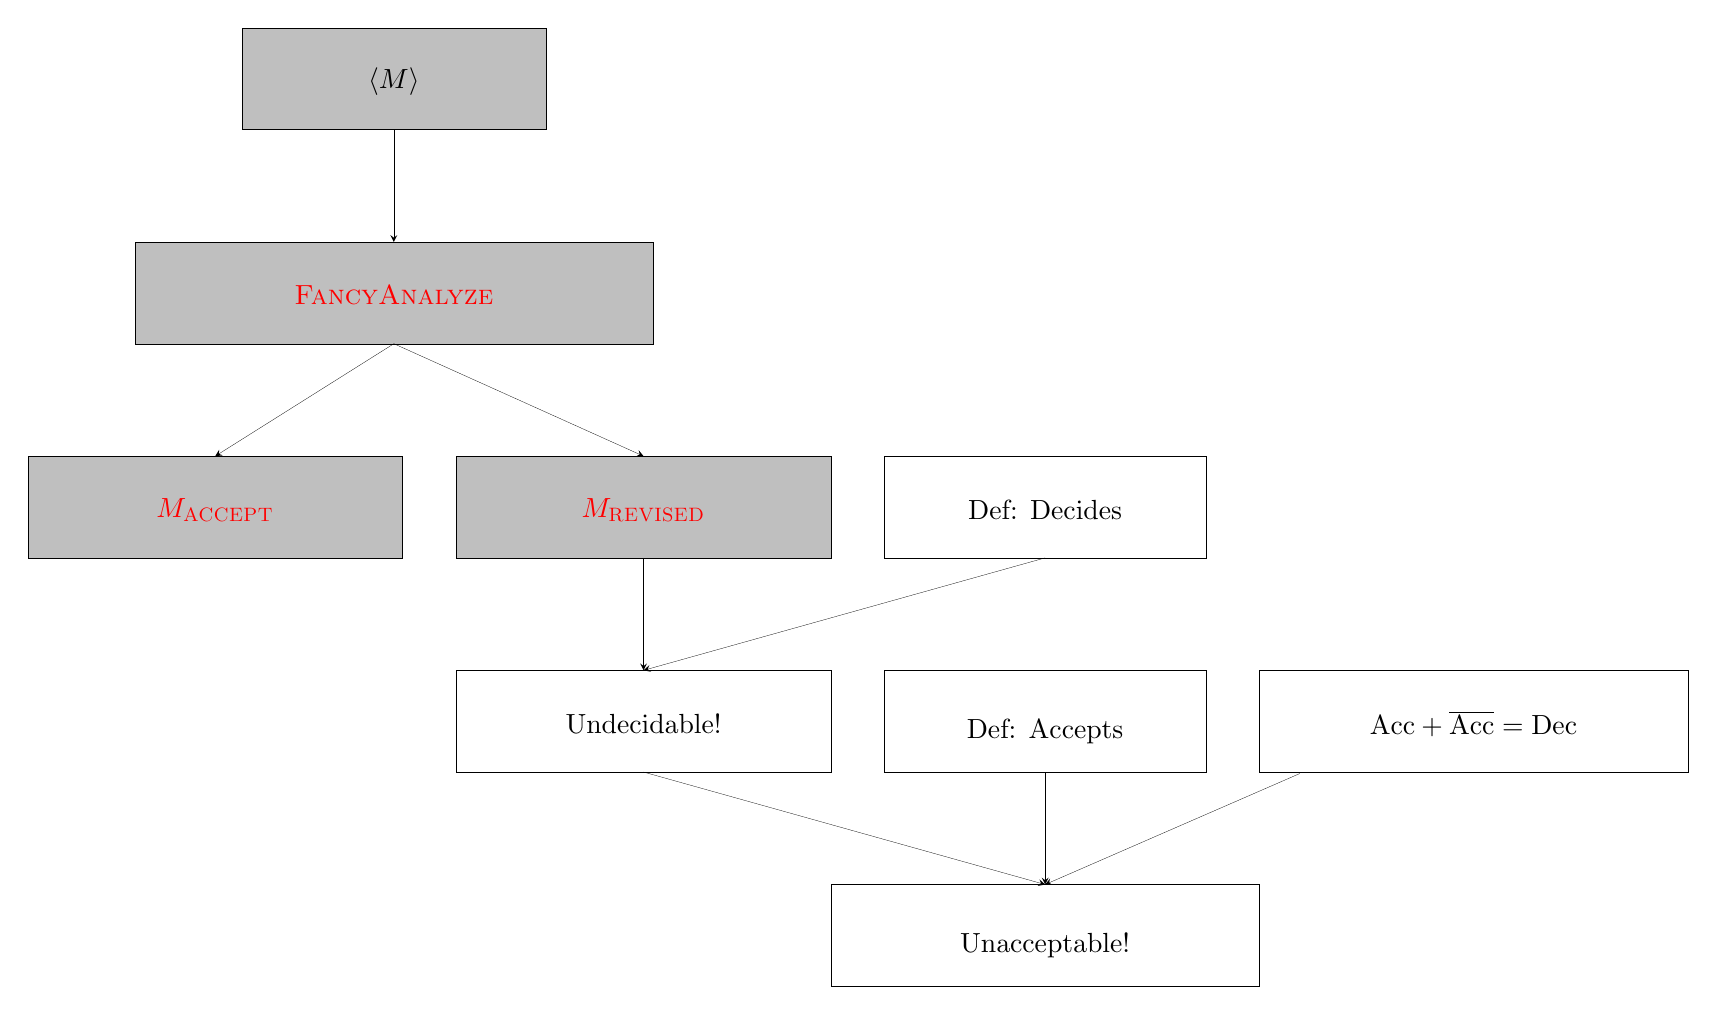
\begin{tikzpicture}
\pgftransformxscale{0.68000}
\pgftransformyscale{-0.680000}
\definecolor{dialinecolor}{rgb}{0.000000, 0.000000, 0.000000}
\pgfsetstrokecolor{dialinecolor}
\definecolor{dialinecolor}{rgb}{1.000000, 1.000000, 1.000000}
\pgfsetfillcolor{dialinecolor}
\definecolor{dialinecolor}{rgb}{1.000000, 1.000000, 1.000000}
\pgfsetfillcolor{black!25}
\fill (12.000000\du,9.000000\du)--(12.000000\du,10.900000\du)--(19.000000\du,10.900000\du)--(19.000000\du,9.000000\du)--cycle;
\pgfsetlinewidth{0.100000\du}
\pgfsetdash{}{0pt}
\pgfsetdash{}{0pt}
\pgfsetmiterjoin
\definecolor{dialinecolor}{rgb}{0.000000, 0.000000, 0.000000}
\pgfsetstrokecolor{dialinecolor}
\draw (12.000000\du,9.000000\du)--(12.000000\du,10.900000\du)--(19.000000\du,10.900000\du)--(19.000000\du,9.000000\du)--cycle;
% setfont left to latex
\definecolor{dialinecolor}{rgb}{0.000000, 0.000000, 0.000000}
\pgfsetstrokecolor{dialinecolor}
\node at (15.500000\du,10.000\du){\MACC};
\definecolor{dialinecolor}{rgb}{1.000000, 1.000000, 1.000000}
\pgfsetfillcolor{black!25}
\fill (20.000000\du,9.000000\du)--(20.000000\du,10.900000\du)--(27.000000\du,10.900000\du)--(27.000000\du,9.000000\du)--cycle;
\pgfsetlinewidth{0.100000\du}
\pgfsetdash{}{0pt}
\pgfsetdash{}{0pt}
\pgfsetmiterjoin
\definecolor{dialinecolor}{rgb}{0.000000, 0.000000, 0.000000}
\pgfsetstrokecolor{dialinecolor}
\draw (20.000000\du,9.000000\du)--(20.000000\du,10.900000\du)--(27.000000\du,10.900000\du)--(27.000000\du,9.000000\du)--cycle;
% setfont left to latex
\definecolor{dialinecolor}{rgb}{0.000000, 0.000000, 0.000000}
\pgfsetstrokecolor{dialinecolor}
\node at (23.500000\du,10.000\du){\MREV};
\definecolor{dialinecolor}{rgb}{1.000000, 1.000000, 1.000000}
\pgfsetfillcolor{dialinecolor}
\fill (35.000000\du,13.000000\du)--(35.000000\du,14.900000\du)--(41.000000\du,14.900000\du)--(41.000000\du,13.000000\du)--cycle;
\pgfsetlinewidth{0.100000\du}
\pgfsetdash{}{0pt}
\pgfsetdash{}{0pt}
\pgfsetmiterjoin
\definecolor{dialinecolor}{rgb}{0.000000, 0.000000, 0.000000}
\pgfsetstrokecolor{dialinecolor}
\draw (35.000000\du,13.000000\du)--(35.000000\du,14.900000\du)--(43.000000\du,14.900000\du)--(43.000000\du,13.000000\du)--cycle;
% setfont left to latex
\definecolor{dialinecolor}{rgb}{0.000000, 0.000000, 0.000000}
\pgfsetstrokecolor{dialinecolor}
\node at (39.000000\du,14.0000\du){$\text{Acc}+\overline{\text{Acc}}=\text{Dec}$};
\definecolor{dialinecolor}{rgb}{1.000000, 1.000000, 1.000000}
\pgfsetfillcolor{black!25}
\fill (14.000000\du,5.000000\du)--(14.000000\du,6.900000\du)--(23.672500\du,6.900000\du)--(23.672500\du,5.000000\du)--cycle;
\pgfsetlinewidth{0.100000\du}
\pgfsetdash{}{0pt}
\pgfsetdash{}{0pt}
\pgfsetmiterjoin
\definecolor{dialinecolor}{rgb}{0.000000, 0.000000, 0.000000}
\pgfsetstrokecolor{dialinecolor}
\draw (14.000000\du,5.000000\du)--(14.000000\du,6.900000\du)--(23.672500\du,6.900000\du)--(23.672500\du,5.000000\du)--cycle;
% setfont left to latex
\definecolor{dialinecolor}{rgb}{0.000000, 0.000000, 0.000000}
\pgfsetstrokecolor{dialinecolor}
\node at (18.836250\du,6.000\du){\func{FancyAnalyze}};
\definecolor{dialinecolor}{rgb}{1.000000, 1.000000, 1.000000}
\pgfsetfillcolor{dialinecolor}
\fill (28.000000\du,13.000000\du)--(28.000000\du,14.900000\du)--(34.000000\du,14.900000\du)--(34.000000\du,13.000000\du)--cycle;
\pgfsetlinewidth{0.100000\du}
\pgfsetdash{}{0pt}
\pgfsetdash{}{0pt}
\pgfsetmiterjoin
\definecolor{dialinecolor}{rgb}{0.000000, 0.000000, 0.000000}
\pgfsetstrokecolor{dialinecolor}
\pgfsetfillcolor{black!25}
\fill (16.000000\du,1.000000\du)--(16.000000\du,2.900000\du)--(21.672500\du,2.900000\du)--(21.672500\du,1.000000\du)--cycle;
\definecolor{dialinecolor}{rgb}{0.000000, 0.000000, 0.000000}\draw (16.000000\du,1.000000\du)--(16.000000\du,2.900000\du)--(21.672500\du,2.900000\du)--(21.672500\du,1.000000\du)--cycle;
% setfont left to latex
\definecolor{dialinecolor}{rgb}{0.000000, 0.000000, 0.000000}
\pgfsetstrokecolor{dialinecolor}
\node at (18.836250\du,2.000\du){\str{M}};
\definecolor{dialinecolor}{rgb}{1.000000, 1.000000, 1.000000}
\pgfsetfillcolor{dialinecolor}
\fill (28.000000\du,13.000000\du)--(28.000000\du,14.900000\du)--(34.000000\du,14.900000\du)--(34.000000\du,13.000000\du)--cycle;
\pgfsetlinewidth{0.100000\du}
\pgfsetdash{}{0pt}
\pgfsetdash{}{0pt}
\pgfsetmiterjoin
\definecolor{dialinecolor}{rgb}{0.000000, 0.000000, 0.000000}
\pgfsetstrokecolor{dialinecolor}
\draw (28.000000\du,13.000000\du)--(28.000000\du,14.900000\du)--(34.000000\du,14.900000\du)--(34.000000\du,13.000000\du)--cycle;
% setfont left to latex
\definecolor{dialinecolor}{rgb}{0.000000, 0.000000, 0.000000}
\pgfsetstrokecolor{dialinecolor}
\node at (31.000000\du,14.145000\du){Def: Accepts};
\definecolor{dialinecolor}{rgb}{1.000000, 1.000000, 1.000000}
\pgfsetfillcolor{dialinecolor}
\fill (28.000000\du,9.000000\du)--(28.000000\du,10.900000\du)--(34.000000\du,10.900000\du)--(34.000000\du,9.000000\du)--cycle;
\pgfsetlinewidth{0.100000\du}
\pgfsetdash{}{0pt}
\pgfsetdash{}{0pt}
\pgfsetmiterjoin
\definecolor{dialinecolor}{rgb}{0.000000, 0.000000, 0.000000}
\pgfsetstrokecolor{dialinecolor}
\draw (28.000000\du,9.000000\du)--(28.000000\du,10.900000\du)--(34.000000\du,10.900000\du)--(34.000000\du,9.000000\du)--cycle;
% setfont left to latex
\definecolor{dialinecolor}{rgb}{0.000000, 0.000000, 0.000000}
\pgfsetstrokecolor{dialinecolor}
\node at (31.000000\du,10.000\du){Def: Decides};
\definecolor{dialinecolor}{rgb}{1.000000, 1.000000, 1.000000}
\pgfsetfillcolor{dialinecolor}
\fill (20.000000\du,13.000000\du)--(20.000000\du,14.900000\du)--(27.000000\du,14.900000\du)--(27.000000\du,13.000000\du)--cycle;
\pgfsetlinewidth{0.100000\du}
\pgfsetdash{}{0pt}
\pgfsetdash{}{0pt}
\pgfsetmiterjoin
\definecolor{dialinecolor}{rgb}{0.000000, 0.000000, 0.000000}
\pgfsetstrokecolor{dialinecolor}
\draw (20.000000\du,13.000000\du)--(20.000000\du,14.900000\du)--(27.000000\du,14.900000\du)--(27.000000\du,13.000000\du)--cycle;
% setfont left to latex
\definecolor{dialinecolor}{rgb}{0.000000, 0.000000, 0.000000}
\pgfsetstrokecolor{dialinecolor}
\node at (23.500000\du,14.000\du){Undecidable!};
\definecolor{dialinecolor}{rgb}{1.000000, 1.000000, 1.000000}
\pgfsetfillcolor{dialinecolor}
\fill (28.000000\du,17.000000\du)--(28.000000\du,18.900000\du)--(34.000000\du,18.900000\du)--(34.000000\du,17.000000\du)--cycle;
\pgfsetlinewidth{0.100000\du}
\pgfsetdash{}{0pt}
\pgfsetdash{}{0pt}
\pgfsetmiterjoin
\definecolor{dialinecolor}{rgb}{0.000000, 0.000000, 0.000000}
\pgfsetstrokecolor{dialinecolor}
\draw (27.000000\du,17.000000\du)--(27.000000\du,18.900000\du)--(35.000000\du,18.900000\du)--(35.000000\du,17.000000\du)--cycle;
% setfont left to latex
\definecolor{dialinecolor}{rgb}{0.000000, 0.000000, 0.000000}
\pgfsetstrokecolor{dialinecolor}
\node at (31.000000\du,18.145000\du){Unacceptable!};
\pgfsetlinewidth{0.100000\du}
\pgfsetdash{}{0pt}
\pgfsetdash{}{0pt}
\pgfsetbuttcap
{
\definecolor{dialinecolor}{rgb}{0.000000, 0.000000, 0.000000}
\pgfsetfillcolor{dialinecolor}
% was here!!!
\pgfsetarrowsend{stealth}
\definecolor{dialinecolor}{rgb}{0.000000, 0.000000, 0.000000}
\pgfsetstrokecolor{dialinecolor}
\draw (18.836250\du,2.900000\du)--(18.836250\du,5.000000\du);
}
\pgfsetlinewidth{0.100000\du}
\pgfsetdash{}{0pt}
\pgfsetdash{}{0pt}
\pgfsetbuttcap
{
\definecolor{dialinecolor}{rgb}{0.000000, 0.000000, 0.000000}
\pgfsetfillcolor{dialinecolor}
% was here!!!
\pgfsetarrowsend{stealth}
\definecolor{dialinecolor}{rgb}{0.000000, 0.000000, 0.000000}
\pgfsetstrokecolor{dialinecolor}
\draw (18.836250\du,6.900000\du)--(15.500000\du,9.000000\du);
}
\pgfsetlinewidth{0.100000\du}
\pgfsetdash{}{0pt}
\pgfsetdash{}{0pt}
\pgfsetbuttcap
{
\definecolor{dialinecolor}{rgb}{0.000000, 0.000000, 0.000000}
\pgfsetfillcolor{dialinecolor}
% was here!!!
\pgfsetarrowsend{stealth}
\definecolor{dialinecolor}{rgb}{0.000000, 0.000000, 0.000000}
\pgfsetstrokecolor{dialinecolor}
\draw (18.836250\du,6.900000\du)--(23.500000\du,9.000000\du);
}
\pgfsetlinewidth{0.100000\du}
\pgfsetdash{}{0pt}
\pgfsetdash{}{0pt}
\pgfsetbuttcap
{
\definecolor{dialinecolor}{rgb}{0.000000, 0.000000, 0.000000}
\pgfsetfillcolor{dialinecolor}
% was here!!!
\pgfsetarrowsend{stealth}
\definecolor{dialinecolor}{rgb}{0.000000, 0.000000, 0.000000}
\pgfsetstrokecolor{dialinecolor}
\draw (23.500000\du,10.900000\du)--(23.500000\du,13.000000\du);
}
\pgfsetlinewidth{0.100000\du}
\pgfsetdash{}{0pt}
\pgfsetdash{}{0pt}
\pgfsetbuttcap
{
\definecolor{dialinecolor}{rgb}{0.000000, 0.000000, 0.000000}
\pgfsetfillcolor{dialinecolor}
% was here!!!
\pgfsetarrowsend{stealth}
\definecolor{dialinecolor}{rgb}{0.000000, 0.000000, 0.000000}
\pgfsetstrokecolor{dialinecolor}
\draw (31.000000\du,10.900000\du)--(23.500000\du,13.000000\du);
}
\pgfsetlinewidth{0.100000\du}
\pgfsetdash{}{0pt}
\pgfsetdash{}{0pt}
\pgfsetbuttcap
{
\definecolor{dialinecolor}{rgb}{0.000000, 0.000000, 0.000000}
\pgfsetfillcolor{dialinecolor}
% was here!!!
\pgfsetarrowsend{stealth}
\definecolor{dialinecolor}{rgb}{0.000000, 0.000000, 0.000000}
\pgfsetstrokecolor{dialinecolor}
\draw (23.500000\du,14.900000\du)--(31.000000\du,17.000000\du);
}
\pgfsetlinewidth{0.100000\du}
\pgfsetdash{}{0pt}
\pgfsetdash{}{0pt}
\pgfsetbuttcap
{
\definecolor{dialinecolor}{rgb}{0.000000, 0.000000, 0.000000}
\pgfsetfillcolor{dialinecolor}
% was here!!!
\pgfsetarrowsend{stealth}
\definecolor{dialinecolor}{rgb}{0.000000, 0.000000, 0.000000}
\pgfsetstrokecolor{dialinecolor}
\draw (31.000000\du,14.900000\du)--(31.000000\du,17.000000\du);
}
\pgfsetlinewidth{0.100000\du}
\pgfsetdash{}{0pt}
\pgfsetdash{}{0pt}
\pgfsetbuttcap
{
\definecolor{dialinecolor}{rgb}{0.000000, 0.000000, 0.000000}
\pgfsetfillcolor{dialinecolor}
% was here!!!
\pgfsetarrowsend{stealth}
\definecolor{dialinecolor}{rgb}{0.000000, 0.000000, 0.000000}
\pgfsetstrokecolor{dialinecolor}
\draw (35.757813\du,14.926953\du)--(31.000000\du,17.000000\du);
}
\end{tikzpicture}
}

\end{frame}

\begin{frame}{The sucker punch}

  What does \MREV~do on input \strMREV?

  \vskip 0.25in

  \MREV(\strMREV) $=$

  \begin{itemize}

  \item If \func{FancyAnalyze}(\strMREV, \strMREV) returns \textit{accept}, then
    \MREV(\strMREV) returns \textit{reject}!

  \item If \func{FancyAnalyze}(\strMREV, \strMREV) returns \textit{reject}, then
    \MREV(\strMREV) returns \textit{accept}!

  \end{itemize}

\end{frame}

\begin{frame}{The sucker punch (in other words)}

  What does \MREV~do on input \strMREV?

  \vskip 0.25in

  \MREV(\strMREV) $=$

  \begin{itemize}

  \item If \MREV~accepts its own description, then it rejects its own
    description!

  \item If \MREV~rejects its own description, then it accepts its own
    description!

  \end{itemize}

\end{frame}

\begin{frame}{What went wrong?}

  % Graphic for TeX using PGF
% Title: C:\Users\Joshua\Documents\teaching\csueb-guest-teaching\flow-diagram.dia
% Creator: Dia v0.97.2
% CreationDate: Tue Feb 04 08:43:25 2014
% For: Joshua
% \usepackage{tikz}
% The following commands are not supported in PSTricks at present
% We define them conditionally, so when they are implemented,
% this pgf file will use them.
\ifx\du\undefined
  \newlength{\du}
\fi
\setlength{\du}{15\unitlength}
{\footnotesize
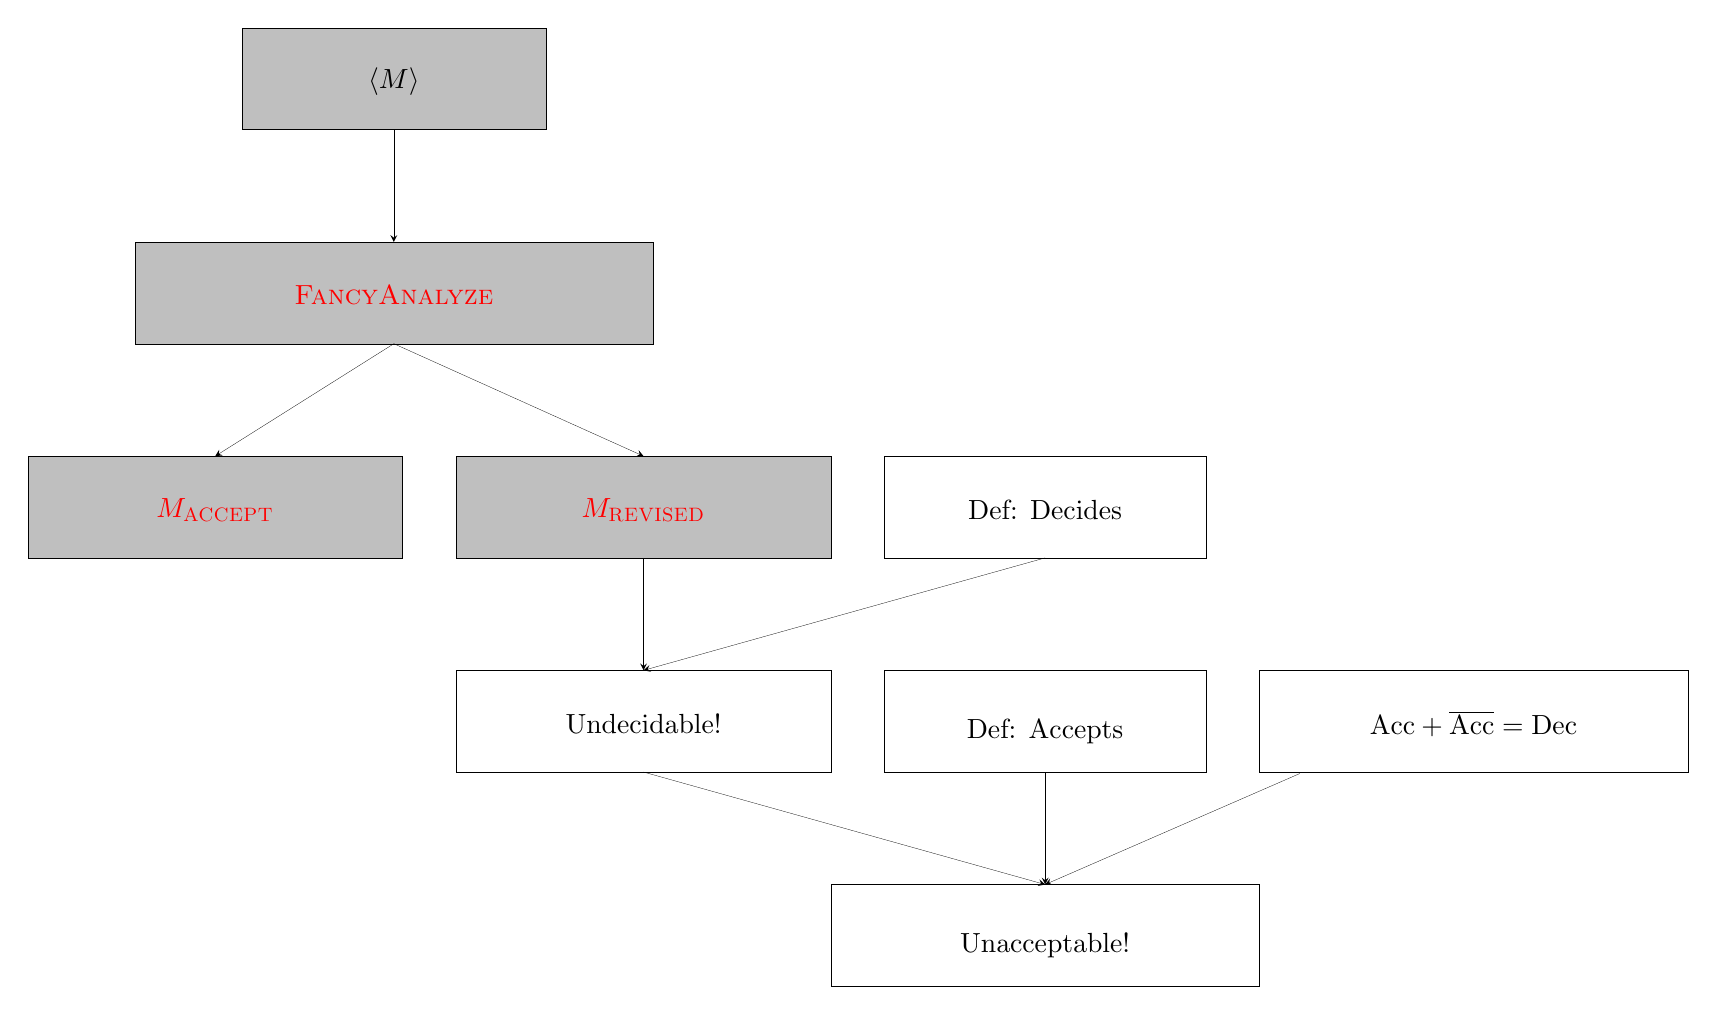
\begin{tikzpicture}
\pgftransformxscale{0.68000}
\pgftransformyscale{-0.680000}
\definecolor{dialinecolor}{rgb}{0.000000, 0.000000, 0.000000}
\pgfsetstrokecolor{dialinecolor}
\definecolor{dialinecolor}{rgb}{1.000000, 1.000000, 1.000000}
\pgfsetfillcolor{dialinecolor}
\definecolor{dialinecolor}{rgb}{1.000000, 1.000000, 1.000000}
\pgfsetfillcolor{black!25}
\fill (12.000000\du,9.000000\du)--(12.000000\du,10.900000\du)--(19.000000\du,10.900000\du)--(19.000000\du,9.000000\du)--cycle;
\pgfsetlinewidth{0.100000\du}
\pgfsetdash{}{0pt}
\pgfsetdash{}{0pt}
\pgfsetmiterjoin
\definecolor{dialinecolor}{rgb}{0.000000, 0.000000, 0.000000}
\pgfsetstrokecolor{dialinecolor}
\draw (12.000000\du,9.000000\du)--(12.000000\du,10.900000\du)--(19.000000\du,10.900000\du)--(19.000000\du,9.000000\du)--cycle;
% setfont left to latex
\definecolor{dialinecolor}{rgb}{0.000000, 0.000000, 0.000000}
\pgfsetstrokecolor{dialinecolor}
\node at (15.500000\du,10.000\du){\MACC};
\definecolor{dialinecolor}{rgb}{1.000000, 1.000000, 1.000000}
\pgfsetfillcolor{black!25}
\fill (20.000000\du,9.000000\du)--(20.000000\du,10.900000\du)--(27.000000\du,10.900000\du)--(27.000000\du,9.000000\du)--cycle;
\pgfsetlinewidth{0.100000\du}
\pgfsetdash{}{0pt}
\pgfsetdash{}{0pt}
\pgfsetmiterjoin
\definecolor{dialinecolor}{rgb}{0.000000, 0.000000, 0.000000}
\pgfsetstrokecolor{dialinecolor}
\draw (20.000000\du,9.000000\du)--(20.000000\du,10.900000\du)--(27.000000\du,10.900000\du)--(27.000000\du,9.000000\du)--cycle;
% setfont left to latex
\definecolor{dialinecolor}{rgb}{0.000000, 0.000000, 0.000000}
\pgfsetstrokecolor{dialinecolor}
\node at (23.500000\du,10.000\du){\MREV};
\definecolor{dialinecolor}{rgb}{1.000000, 1.000000, 1.000000}
\pgfsetfillcolor{dialinecolor}
\fill (35.000000\du,13.000000\du)--(35.000000\du,14.900000\du)--(41.000000\du,14.900000\du)--(41.000000\du,13.000000\du)--cycle;
\pgfsetlinewidth{0.100000\du}
\pgfsetdash{}{0pt}
\pgfsetdash{}{0pt}
\pgfsetmiterjoin
\definecolor{dialinecolor}{rgb}{0.000000, 0.000000, 0.000000}
\pgfsetstrokecolor{dialinecolor}
\draw (35.000000\du,13.000000\du)--(35.000000\du,14.900000\du)--(43.000000\du,14.900000\du)--(43.000000\du,13.000000\du)--cycle;
% setfont left to latex
\definecolor{dialinecolor}{rgb}{0.000000, 0.000000, 0.000000}
\pgfsetstrokecolor{dialinecolor}
\node at (39.000000\du,14.0000\du){$\text{Acc}+\overline{\text{Acc}}=\text{Dec}$};
\definecolor{dialinecolor}{rgb}{1.000000, 1.000000, 1.000000}
\pgfsetfillcolor{black!25}
\fill (14.000000\du,5.000000\du)--(14.000000\du,6.900000\du)--(23.672500\du,6.900000\du)--(23.672500\du,5.000000\du)--cycle;
\pgfsetlinewidth{0.100000\du}
\pgfsetdash{}{0pt}
\pgfsetdash{}{0pt}
\pgfsetmiterjoin
\definecolor{dialinecolor}{rgb}{0.000000, 0.000000, 0.000000}
\pgfsetstrokecolor{dialinecolor}
\draw (14.000000\du,5.000000\du)--(14.000000\du,6.900000\du)--(23.672500\du,6.900000\du)--(23.672500\du,5.000000\du)--cycle;
% setfont left to latex
\definecolor{dialinecolor}{rgb}{0.000000, 0.000000, 0.000000}
\pgfsetstrokecolor{dialinecolor}
\node at (18.836250\du,6.000\du){\func{FancyAnalyze}};
\definecolor{dialinecolor}{rgb}{1.000000, 1.000000, 1.000000}
\pgfsetfillcolor{dialinecolor}
\fill (28.000000\du,13.000000\du)--(28.000000\du,14.900000\du)--(34.000000\du,14.900000\du)--(34.000000\du,13.000000\du)--cycle;
\pgfsetlinewidth{0.100000\du}
\pgfsetdash{}{0pt}
\pgfsetdash{}{0pt}
\pgfsetmiterjoin
\definecolor{dialinecolor}{rgb}{0.000000, 0.000000, 0.000000}
\pgfsetstrokecolor{dialinecolor}
\pgfsetfillcolor{black!25}
\fill (16.000000\du,1.000000\du)--(16.000000\du,2.900000\du)--(21.672500\du,2.900000\du)--(21.672500\du,1.000000\du)--cycle;
\definecolor{dialinecolor}{rgb}{0.000000, 0.000000, 0.000000}\draw (16.000000\du,1.000000\du)--(16.000000\du,2.900000\du)--(21.672500\du,2.900000\du)--(21.672500\du,1.000000\du)--cycle;
% setfont left to latex
\definecolor{dialinecolor}{rgb}{0.000000, 0.000000, 0.000000}
\pgfsetstrokecolor{dialinecolor}
\node at (18.836250\du,2.000\du){\str{M}};
\definecolor{dialinecolor}{rgb}{1.000000, 1.000000, 1.000000}
\pgfsetfillcolor{dialinecolor}
\fill (28.000000\du,13.000000\du)--(28.000000\du,14.900000\du)--(34.000000\du,14.900000\du)--(34.000000\du,13.000000\du)--cycle;
\pgfsetlinewidth{0.100000\du}
\pgfsetdash{}{0pt}
\pgfsetdash{}{0pt}
\pgfsetmiterjoin
\definecolor{dialinecolor}{rgb}{0.000000, 0.000000, 0.000000}
\pgfsetstrokecolor{dialinecolor}
\draw (28.000000\du,13.000000\du)--(28.000000\du,14.900000\du)--(34.000000\du,14.900000\du)--(34.000000\du,13.000000\du)--cycle;
% setfont left to latex
\definecolor{dialinecolor}{rgb}{0.000000, 0.000000, 0.000000}
\pgfsetstrokecolor{dialinecolor}
\node at (31.000000\du,14.145000\du){Def: Accepts};
\definecolor{dialinecolor}{rgb}{1.000000, 1.000000, 1.000000}
\pgfsetfillcolor{dialinecolor}
\fill (28.000000\du,9.000000\du)--(28.000000\du,10.900000\du)--(34.000000\du,10.900000\du)--(34.000000\du,9.000000\du)--cycle;
\pgfsetlinewidth{0.100000\du}
\pgfsetdash{}{0pt}
\pgfsetdash{}{0pt}
\pgfsetmiterjoin
\definecolor{dialinecolor}{rgb}{0.000000, 0.000000, 0.000000}
\pgfsetstrokecolor{dialinecolor}
\draw (28.000000\du,9.000000\du)--(28.000000\du,10.900000\du)--(34.000000\du,10.900000\du)--(34.000000\du,9.000000\du)--cycle;
% setfont left to latex
\definecolor{dialinecolor}{rgb}{0.000000, 0.000000, 0.000000}
\pgfsetstrokecolor{dialinecolor}
\node at (31.000000\du,10.000\du){Def: Decides};
\definecolor{dialinecolor}{rgb}{1.000000, 1.000000, 1.000000}
\pgfsetfillcolor{dialinecolor}
\fill (20.000000\du,13.000000\du)--(20.000000\du,14.900000\du)--(27.000000\du,14.900000\du)--(27.000000\du,13.000000\du)--cycle;
\pgfsetlinewidth{0.100000\du}
\pgfsetdash{}{0pt}
\pgfsetdash{}{0pt}
\pgfsetmiterjoin
\definecolor{dialinecolor}{rgb}{0.000000, 0.000000, 0.000000}
\pgfsetstrokecolor{dialinecolor}
\draw (20.000000\du,13.000000\du)--(20.000000\du,14.900000\du)--(27.000000\du,14.900000\du)--(27.000000\du,13.000000\du)--cycle;
% setfont left to latex
\definecolor{dialinecolor}{rgb}{0.000000, 0.000000, 0.000000}
\pgfsetstrokecolor{dialinecolor}
\node at (23.500000\du,14.000\du){Undecidable!};
\definecolor{dialinecolor}{rgb}{1.000000, 1.000000, 1.000000}
\pgfsetfillcolor{dialinecolor}
\fill (28.000000\du,17.000000\du)--(28.000000\du,18.900000\du)--(34.000000\du,18.900000\du)--(34.000000\du,17.000000\du)--cycle;
\pgfsetlinewidth{0.100000\du}
\pgfsetdash{}{0pt}
\pgfsetdash{}{0pt}
\pgfsetmiterjoin
\definecolor{dialinecolor}{rgb}{0.000000, 0.000000, 0.000000}
\pgfsetstrokecolor{dialinecolor}
\draw (27.000000\du,17.000000\du)--(27.000000\du,18.900000\du)--(35.000000\du,18.900000\du)--(35.000000\du,17.000000\du)--cycle;
% setfont left to latex
\definecolor{dialinecolor}{rgb}{0.000000, 0.000000, 0.000000}
\pgfsetstrokecolor{dialinecolor}
\node at (31.000000\du,18.145000\du){Unacceptable!};
\pgfsetlinewidth{0.100000\du}
\pgfsetdash{}{0pt}
\pgfsetdash{}{0pt}
\pgfsetbuttcap
{
\definecolor{dialinecolor}{rgb}{0.000000, 0.000000, 0.000000}
\pgfsetfillcolor{dialinecolor}
% was here!!!
\pgfsetarrowsend{stealth}
\definecolor{dialinecolor}{rgb}{0.000000, 0.000000, 0.000000}
\pgfsetstrokecolor{dialinecolor}
\draw (18.836250\du,2.900000\du)--(18.836250\du,5.000000\du);
}
\pgfsetlinewidth{0.100000\du}
\pgfsetdash{}{0pt}
\pgfsetdash{}{0pt}
\pgfsetbuttcap
{
\definecolor{dialinecolor}{rgb}{0.000000, 0.000000, 0.000000}
\pgfsetfillcolor{dialinecolor}
% was here!!!
\pgfsetarrowsend{stealth}
\definecolor{dialinecolor}{rgb}{0.000000, 0.000000, 0.000000}
\pgfsetstrokecolor{dialinecolor}
\draw (18.836250\du,6.900000\du)--(15.500000\du,9.000000\du);
}
\pgfsetlinewidth{0.100000\du}
\pgfsetdash{}{0pt}
\pgfsetdash{}{0pt}
\pgfsetbuttcap
{
\definecolor{dialinecolor}{rgb}{0.000000, 0.000000, 0.000000}
\pgfsetfillcolor{dialinecolor}
% was here!!!
\pgfsetarrowsend{stealth}
\definecolor{dialinecolor}{rgb}{0.000000, 0.000000, 0.000000}
\pgfsetstrokecolor{dialinecolor}
\draw (18.836250\du,6.900000\du)--(23.500000\du,9.000000\du);
}
\pgfsetlinewidth{0.100000\du}
\pgfsetdash{}{0pt}
\pgfsetdash{}{0pt}
\pgfsetbuttcap
{
\definecolor{dialinecolor}{rgb}{0.000000, 0.000000, 0.000000}
\pgfsetfillcolor{dialinecolor}
% was here!!!
\pgfsetarrowsend{stealth}
\definecolor{dialinecolor}{rgb}{0.000000, 0.000000, 0.000000}
\pgfsetstrokecolor{dialinecolor}
\draw (23.500000\du,10.900000\du)--(23.500000\du,13.000000\du);
}
\pgfsetlinewidth{0.100000\du}
\pgfsetdash{}{0pt}
\pgfsetdash{}{0pt}
\pgfsetbuttcap
{
\definecolor{dialinecolor}{rgb}{0.000000, 0.000000, 0.000000}
\pgfsetfillcolor{dialinecolor}
% was here!!!
\pgfsetarrowsend{stealth}
\definecolor{dialinecolor}{rgb}{0.000000, 0.000000, 0.000000}
\pgfsetstrokecolor{dialinecolor}
\draw (31.000000\du,10.900000\du)--(23.500000\du,13.000000\du);
}
\pgfsetlinewidth{0.100000\du}
\pgfsetdash{}{0pt}
\pgfsetdash{}{0pt}
\pgfsetbuttcap
{
\definecolor{dialinecolor}{rgb}{0.000000, 0.000000, 0.000000}
\pgfsetfillcolor{dialinecolor}
% was here!!!
\pgfsetarrowsend{stealth}
\definecolor{dialinecolor}{rgb}{0.000000, 0.000000, 0.000000}
\pgfsetstrokecolor{dialinecolor}
\draw (23.500000\du,14.900000\du)--(31.000000\du,17.000000\du);
}
\pgfsetlinewidth{0.100000\du}
\pgfsetdash{}{0pt}
\pgfsetdash{}{0pt}
\pgfsetbuttcap
{
\definecolor{dialinecolor}{rgb}{0.000000, 0.000000, 0.000000}
\pgfsetfillcolor{dialinecolor}
% was here!!!
\pgfsetarrowsend{stealth}
\definecolor{dialinecolor}{rgb}{0.000000, 0.000000, 0.000000}
\pgfsetstrokecolor{dialinecolor}
\draw (31.000000\du,14.900000\du)--(31.000000\du,17.000000\du);
}
\pgfsetlinewidth{0.100000\du}
\pgfsetdash{}{0pt}
\pgfsetdash{}{0pt}
\pgfsetbuttcap
{
\definecolor{dialinecolor}{rgb}{0.000000, 0.000000, 0.000000}
\pgfsetfillcolor{dialinecolor}
% was here!!!
\pgfsetarrowsend{stealth}
\definecolor{dialinecolor}{rgb}{0.000000, 0.000000, 0.000000}
\pgfsetstrokecolor{dialinecolor}
\draw (35.757813\du,14.926953\du)--(31.000000\du,17.000000\du);
}
\end{tikzpicture}
}

\end{frame}

\begin{frame}{Definition: Decides}

  foobar

\end{frame}

\begin{frame}{The Plan}

  % Graphic for TeX using PGF
% Title: C:\Users\Joshua\Documents\teaching\csueb-guest-teaching\flow-diagram.dia
% Creator: Dia v0.97.2
% CreationDate: Tue Feb 04 08:43:25 2014
% For: Joshua
% \usepackage{tikz}
% The following commands are not supported in PSTricks at present
% We define them conditionally, so when they are implemented,
% this pgf file will use them.
\ifx\du\undefined
  \newlength{\du}
\fi
\setlength{\du}{15\unitlength}
{\footnotesize
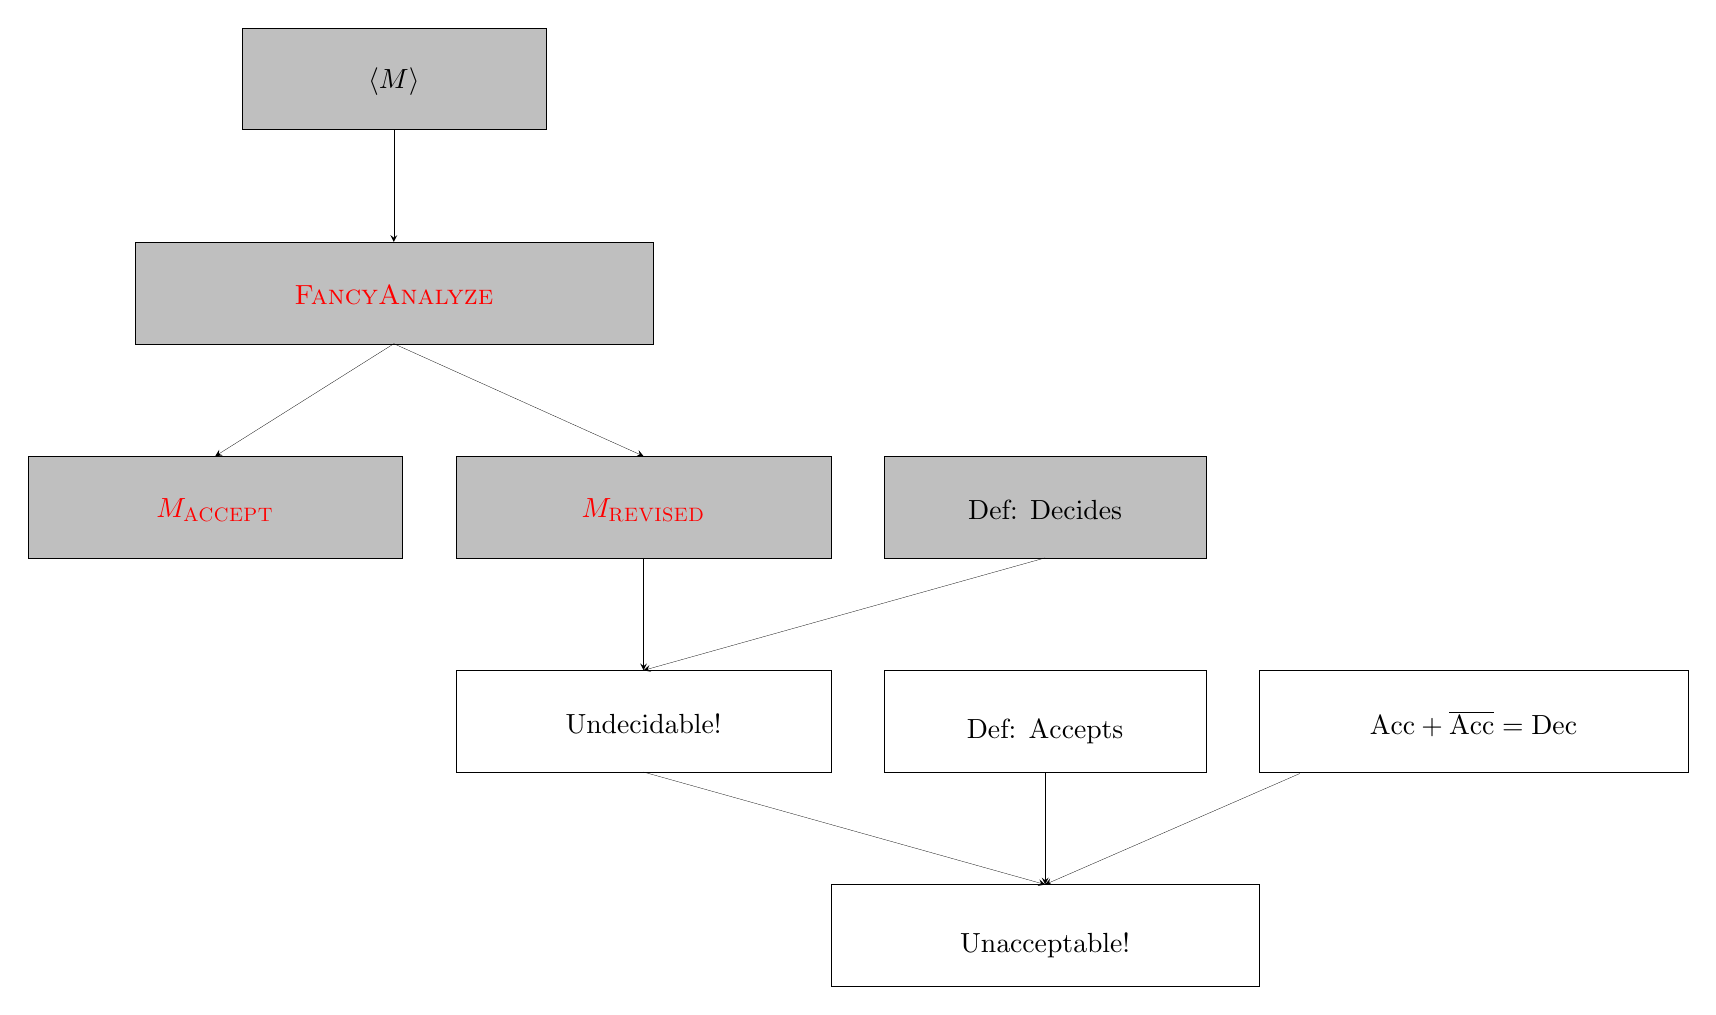
\begin{tikzpicture}
\pgftransformxscale{0.68000}
\pgftransformyscale{-0.680000}
\definecolor{dialinecolor}{rgb}{0.000000, 0.000000, 0.000000}
\pgfsetstrokecolor{dialinecolor}
\definecolor{dialinecolor}{rgb}{1.000000, 1.000000, 1.000000}
\pgfsetfillcolor{dialinecolor}
\definecolor{dialinecolor}{rgb}{1.000000, 1.000000, 1.000000}
\pgfsetfillcolor{black!25}
\fill (12.000000\du,9.000000\du)--(12.000000\du,10.900000\du)--(19.000000\du,10.900000\du)--(19.000000\du,9.000000\du)--cycle;
\pgfsetlinewidth{0.100000\du}
\pgfsetdash{}{0pt}
\pgfsetdash{}{0pt}
\pgfsetmiterjoin
\definecolor{dialinecolor}{rgb}{0.000000, 0.000000, 0.000000}
\pgfsetstrokecolor{dialinecolor}
\draw (12.000000\du,9.000000\du)--(12.000000\du,10.900000\du)--(19.000000\du,10.900000\du)--(19.000000\du,9.000000\du)--cycle;
% setfont left to latex
\definecolor{dialinecolor}{rgb}{0.000000, 0.000000, 0.000000}
\pgfsetstrokecolor{dialinecolor}
\node at (15.500000\du,10.000\du){\MACC};
\definecolor{dialinecolor}{rgb}{1.000000, 1.000000, 1.000000}
\pgfsetfillcolor{black!25}
\fill (20.000000\du,9.000000\du)--(20.000000\du,10.900000\du)--(27.000000\du,10.900000\du)--(27.000000\du,9.000000\du)--cycle;
\pgfsetlinewidth{0.100000\du}
\pgfsetdash{}{0pt}
\pgfsetdash{}{0pt}
\pgfsetmiterjoin
\definecolor{dialinecolor}{rgb}{0.000000, 0.000000, 0.000000}
\pgfsetstrokecolor{dialinecolor}
\draw (20.000000\du,9.000000\du)--(20.000000\du,10.900000\du)--(27.000000\du,10.900000\du)--(27.000000\du,9.000000\du)--cycle;
% setfont left to latex
\definecolor{dialinecolor}{rgb}{0.000000, 0.000000, 0.000000}
\pgfsetstrokecolor{dialinecolor}
\node at (23.500000\du,10.000\du){\MREV};
\definecolor{dialinecolor}{rgb}{1.000000, 1.000000, 1.000000}
\pgfsetfillcolor{dialinecolor}
\fill (35.000000\du,13.000000\du)--(35.000000\du,14.900000\du)--(41.000000\du,14.900000\du)--(41.000000\du,13.000000\du)--cycle;
\pgfsetlinewidth{0.100000\du}
\pgfsetdash{}{0pt}
\pgfsetdash{}{0pt}
\pgfsetmiterjoin
\definecolor{dialinecolor}{rgb}{0.000000, 0.000000, 0.000000}
\pgfsetstrokecolor{dialinecolor}
\draw (35.000000\du,13.000000\du)--(35.000000\du,14.900000\du)--(43.000000\du,14.900000\du)--(43.000000\du,13.000000\du)--cycle;
% setfont left to latex
\definecolor{dialinecolor}{rgb}{0.000000, 0.000000, 0.000000}
\pgfsetstrokecolor{dialinecolor}
\node at (39.000000\du,14.0000\du){$\text{Acc}+\overline{\text{Acc}}=\text{Dec}$};
\definecolor{dialinecolor}{rgb}{1.000000, 1.000000, 1.000000}
\pgfsetfillcolor{black!25}
\fill (14.000000\du,5.000000\du)--(14.000000\du,6.900000\du)--(23.672500\du,6.900000\du)--(23.672500\du,5.000000\du)--cycle;
\pgfsetlinewidth{0.100000\du}
\pgfsetdash{}{0pt}
\pgfsetdash{}{0pt}
\pgfsetmiterjoin
\definecolor{dialinecolor}{rgb}{0.000000, 0.000000, 0.000000}
\pgfsetstrokecolor{dialinecolor}
\draw (14.000000\du,5.000000\du)--(14.000000\du,6.900000\du)--(23.672500\du,6.900000\du)--(23.672500\du,5.000000\du)--cycle;
% setfont left to latex
\definecolor{dialinecolor}{rgb}{0.000000, 0.000000, 0.000000}
\pgfsetstrokecolor{dialinecolor}
\node at (18.836250\du,6.000\du){\func{FancyAnalyze}};
\definecolor{dialinecolor}{rgb}{1.000000, 1.000000, 1.000000}
\pgfsetfillcolor{dialinecolor}
\fill (28.000000\du,13.000000\du)--(28.000000\du,14.900000\du)--(34.000000\du,14.900000\du)--(34.000000\du,13.000000\du)--cycle;
\pgfsetlinewidth{0.100000\du}
\pgfsetdash{}{0pt}
\pgfsetdash{}{0pt}
\pgfsetmiterjoin
\definecolor{dialinecolor}{rgb}{0.000000, 0.000000, 0.000000}
\pgfsetstrokecolor{dialinecolor}
\pgfsetfillcolor{black!25}
\fill (16.000000\du,1.000000\du)--(16.000000\du,2.900000\du)--(21.672500\du,2.900000\du)--(21.672500\du,1.000000\du)--cycle;
\definecolor{dialinecolor}{rgb}{0.000000, 0.000000, 0.000000}\draw (16.000000\du,1.000000\du)--(16.000000\du,2.900000\du)--(21.672500\du,2.900000\du)--(21.672500\du,1.000000\du)--cycle;
% setfont left to latex
\definecolor{dialinecolor}{rgb}{0.000000, 0.000000, 0.000000}
\pgfsetstrokecolor{dialinecolor}
\node at (18.836250\du,2.000\du){\str{M}};
\definecolor{dialinecolor}{rgb}{1.000000, 1.000000, 1.000000}
\pgfsetfillcolor{dialinecolor}
\fill (28.000000\du,13.000000\du)--(28.000000\du,14.900000\du)--(34.000000\du,14.900000\du)--(34.000000\du,13.000000\du)--cycle;
\pgfsetlinewidth{0.100000\du}
\pgfsetdash{}{0pt}
\pgfsetdash{}{0pt}
\pgfsetmiterjoin
\definecolor{dialinecolor}{rgb}{0.000000, 0.000000, 0.000000}
\pgfsetstrokecolor{dialinecolor}
\draw (28.000000\du,13.000000\du)--(28.000000\du,14.900000\du)--(34.000000\du,14.900000\du)--(34.000000\du,13.000000\du)--cycle;
% setfont left to latex
\definecolor{dialinecolor}{rgb}{0.000000, 0.000000, 0.000000}
\pgfsetstrokecolor{dialinecolor}
\node at (31.000000\du,14.145000\du){Def: Accepts};
\definecolor{dialinecolor}{rgb}{1.000000, 1.000000, 1.000000}
\pgfsetfillcolor{black!25}
\fill (28.000000\du,9.000000\du)--(28.000000\du,10.900000\du)--(34.000000\du,10.900000\du)--(34.000000\du,9.000000\du)--cycle;
\pgfsetlinewidth{0.100000\du}
\pgfsetdash{}{0pt}
\pgfsetdash{}{0pt}
\pgfsetmiterjoin
\definecolor{dialinecolor}{rgb}{0.000000, 0.000000, 0.000000}
\pgfsetstrokecolor{dialinecolor}
\draw (28.000000\du,9.000000\du)--(28.000000\du,10.900000\du)--(34.000000\du,10.900000\du)--(34.000000\du,9.000000\du)--cycle;
% setfont left to latex
\definecolor{dialinecolor}{rgb}{0.000000, 0.000000, 0.000000}
\pgfsetstrokecolor{dialinecolor}
\node at (31.000000\du,10.000\du){Def: Decides};
\definecolor{dialinecolor}{rgb}{1.000000, 1.000000, 1.000000}
\pgfsetfillcolor{dialinecolor}
\fill (20.000000\du,13.000000\du)--(20.000000\du,14.900000\du)--(27.000000\du,14.900000\du)--(27.000000\du,13.000000\du)--cycle;
\pgfsetlinewidth{0.100000\du}
\pgfsetdash{}{0pt}
\pgfsetdash{}{0pt}
\pgfsetmiterjoin
\definecolor{dialinecolor}{rgb}{0.000000, 0.000000, 0.000000}
\pgfsetstrokecolor{dialinecolor}
\draw (20.000000\du,13.000000\du)--(20.000000\du,14.900000\du)--(27.000000\du,14.900000\du)--(27.000000\du,13.000000\du)--cycle;
% setfont left to latex
\definecolor{dialinecolor}{rgb}{0.000000, 0.000000, 0.000000}
\pgfsetstrokecolor{dialinecolor}
\node at (23.500000\du,14.000\du){Undecidable!};
\definecolor{dialinecolor}{rgb}{1.000000, 1.000000, 1.000000}
\pgfsetfillcolor{dialinecolor}
\fill (28.000000\du,17.000000\du)--(28.000000\du,18.900000\du)--(34.000000\du,18.900000\du)--(34.000000\du,17.000000\du)--cycle;
\pgfsetlinewidth{0.100000\du}
\pgfsetdash{}{0pt}
\pgfsetdash{}{0pt}
\pgfsetmiterjoin
\definecolor{dialinecolor}{rgb}{0.000000, 0.000000, 0.000000}
\pgfsetstrokecolor{dialinecolor}
\draw (27.000000\du,17.000000\du)--(27.000000\du,18.900000\du)--(35.000000\du,18.900000\du)--(35.000000\du,17.000000\du)--cycle;
% setfont left to latex
\definecolor{dialinecolor}{rgb}{0.000000, 0.000000, 0.000000}
\pgfsetstrokecolor{dialinecolor}
\node at (31.000000\du,18.145000\du){Unacceptable!};
\pgfsetlinewidth{0.100000\du}
\pgfsetdash{}{0pt}
\pgfsetdash{}{0pt}
\pgfsetbuttcap
{
\definecolor{dialinecolor}{rgb}{0.000000, 0.000000, 0.000000}
\pgfsetfillcolor{dialinecolor}
% was here!!!
\pgfsetarrowsend{stealth}
\definecolor{dialinecolor}{rgb}{0.000000, 0.000000, 0.000000}
\pgfsetstrokecolor{dialinecolor}
\draw (18.836250\du,2.900000\du)--(18.836250\du,5.000000\du);
}
\pgfsetlinewidth{0.100000\du}
\pgfsetdash{}{0pt}
\pgfsetdash{}{0pt}
\pgfsetbuttcap
{
\definecolor{dialinecolor}{rgb}{0.000000, 0.000000, 0.000000}
\pgfsetfillcolor{dialinecolor}
% was here!!!
\pgfsetarrowsend{stealth}
\definecolor{dialinecolor}{rgb}{0.000000, 0.000000, 0.000000}
\pgfsetstrokecolor{dialinecolor}
\draw (18.836250\du,6.900000\du)--(15.500000\du,9.000000\du);
}
\pgfsetlinewidth{0.100000\du}
\pgfsetdash{}{0pt}
\pgfsetdash{}{0pt}
\pgfsetbuttcap
{
\definecolor{dialinecolor}{rgb}{0.000000, 0.000000, 0.000000}
\pgfsetfillcolor{dialinecolor}
% was here!!!
\pgfsetarrowsend{stealth}
\definecolor{dialinecolor}{rgb}{0.000000, 0.000000, 0.000000}
\pgfsetstrokecolor{dialinecolor}
\draw (18.836250\du,6.900000\du)--(23.500000\du,9.000000\du);
}
\pgfsetlinewidth{0.100000\du}
\pgfsetdash{}{0pt}
\pgfsetdash{}{0pt}
\pgfsetbuttcap
{
\definecolor{dialinecolor}{rgb}{0.000000, 0.000000, 0.000000}
\pgfsetfillcolor{dialinecolor}
% was here!!!
\pgfsetarrowsend{stealth}
\definecolor{dialinecolor}{rgb}{0.000000, 0.000000, 0.000000}
\pgfsetstrokecolor{dialinecolor}
\draw (23.500000\du,10.900000\du)--(23.500000\du,13.000000\du);
}
\pgfsetlinewidth{0.100000\du}
\pgfsetdash{}{0pt}
\pgfsetdash{}{0pt}
\pgfsetbuttcap
{
\definecolor{dialinecolor}{rgb}{0.000000, 0.000000, 0.000000}
\pgfsetfillcolor{dialinecolor}
% was here!!!
\pgfsetarrowsend{stealth}
\definecolor{dialinecolor}{rgb}{0.000000, 0.000000, 0.000000}
\pgfsetstrokecolor{dialinecolor}
\draw (31.000000\du,10.900000\du)--(23.500000\du,13.000000\du);
}
\pgfsetlinewidth{0.100000\du}
\pgfsetdash{}{0pt}
\pgfsetdash{}{0pt}
\pgfsetbuttcap
{
\definecolor{dialinecolor}{rgb}{0.000000, 0.000000, 0.000000}
\pgfsetfillcolor{dialinecolor}
% was here!!!
\pgfsetarrowsend{stealth}
\definecolor{dialinecolor}{rgb}{0.000000, 0.000000, 0.000000}
\pgfsetstrokecolor{dialinecolor}
\draw (23.500000\du,14.900000\du)--(31.000000\du,17.000000\du);
}
\pgfsetlinewidth{0.100000\du}
\pgfsetdash{}{0pt}
\pgfsetdash{}{0pt}
\pgfsetbuttcap
{
\definecolor{dialinecolor}{rgb}{0.000000, 0.000000, 0.000000}
\pgfsetfillcolor{dialinecolor}
% was here!!!
\pgfsetarrowsend{stealth}
\definecolor{dialinecolor}{rgb}{0.000000, 0.000000, 0.000000}
\pgfsetstrokecolor{dialinecolor}
\draw (31.000000\du,14.900000\du)--(31.000000\du,17.000000\du);
}
\pgfsetlinewidth{0.100000\du}
\pgfsetdash{}{0pt}
\pgfsetdash{}{0pt}
\pgfsetbuttcap
{
\definecolor{dialinecolor}{rgb}{0.000000, 0.000000, 0.000000}
\pgfsetfillcolor{dialinecolor}
% was here!!!
\pgfsetarrowsend{stealth}
\definecolor{dialinecolor}{rgb}{0.000000, 0.000000, 0.000000}
\pgfsetstrokecolor{dialinecolor}
\draw (35.757813\du,14.926953\du)--(31.000000\du,17.000000\du);
}
\end{tikzpicture}
}

\end{frame}

\begin{frame}{Undecidable!}

  So \func{FancyAnalyze} cannot exist (as a decider). The \textit{language}
  it would have decided was,

  \begin{equation*}
    \text{ACCEPT}_{\text{TM}} = \{ (\langle M \rangle, w) : M \text{
      accepts } w\}.
  \end{equation*}

  \vskip 0.25in

  However, $\text{ACCEPT}_{\text{TM}}$ is easy to \textit{accept}. Just
  literally simulate $M$ on $w$ (if $M$ accepts $w$, so does the
  simulator).

\end{frame}

\begin{frame}{The Halting Problem}

  \func{FancyAnalyze}(\str{M}, $w$) could have been written differently:

  \begin{itemize}

  \item If $M$ halts on $w$ (accepts or rejects $w$), then \func{FancyAnalyze} halts.

  \item Otherwise, loop forever.

  \end{itemize}

\end{frame}

\begin{frame}{The Halting Problem}

  Then we make a variant, \func{WackoAnalyze}, that does the opposite
  (loops forever if $M$ halts, and halts if $M$ loops forever).

  \vskip 0.25in

  Now, \func{WackoAnalyze}, when executed on its own description,
  halts when it loops forever and loops forever when it halts (!).

\end{frame}

\begin{frame}{Undecidable!}

  Either way, we have an undecidable problem (i.e., undecidable
  language).

\end{frame}

\begin{frame}{The Plan}

  % Graphic for TeX using PGF
% Title: C:\Users\Joshua\Documents\teaching\csueb-guest-teaching\flow-diagram.dia
% Creator: Dia v0.97.2
% CreationDate: Tue Feb 04 08:43:25 2014
% For: Joshua
% \usepackage{tikz}
% The following commands are not supported in PSTricks at present
% We define them conditionally, so when they are implemented,
% this pgf file will use them.
\ifx\du\undefined
  \newlength{\du}
\fi
\setlength{\du}{15\unitlength}
{\footnotesize
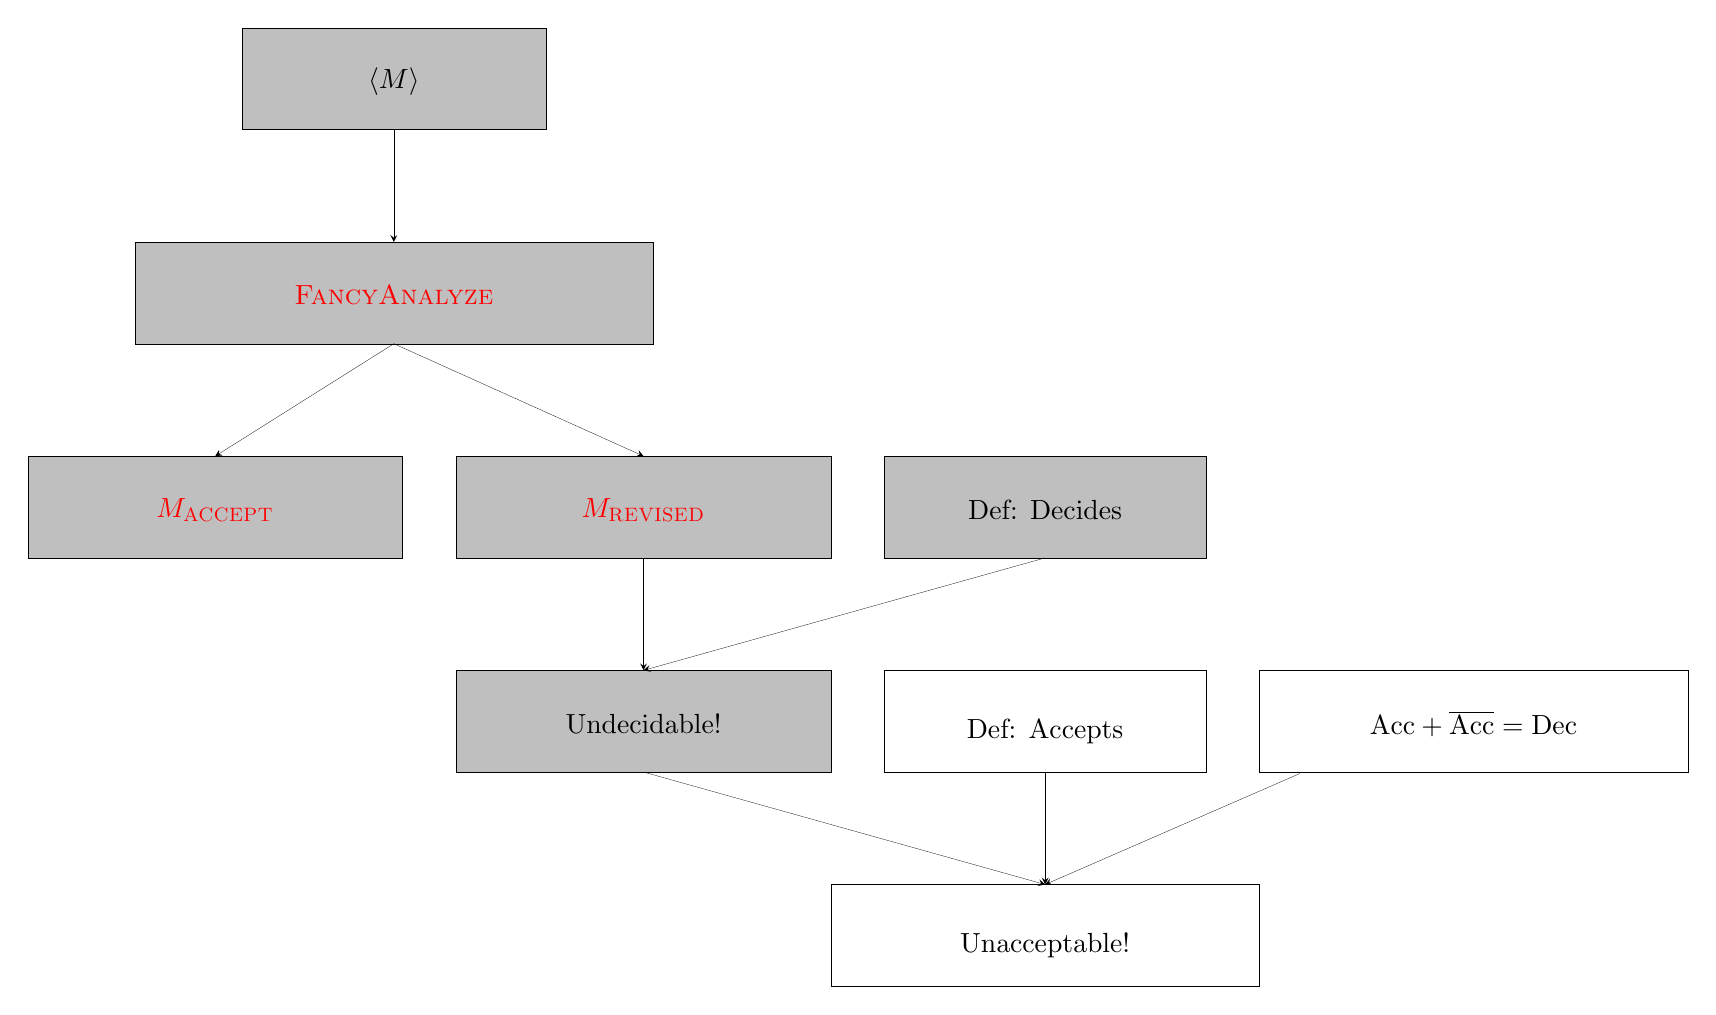
\begin{tikzpicture}
\pgftransformxscale{0.68000}
\pgftransformyscale{-0.680000}
\definecolor{dialinecolor}{rgb}{0.000000, 0.000000, 0.000000}
\pgfsetstrokecolor{dialinecolor}
\definecolor{dialinecolor}{rgb}{1.000000, 1.000000, 1.000000}
\pgfsetfillcolor{dialinecolor}
\definecolor{dialinecolor}{rgb}{1.000000, 1.000000, 1.000000}
\pgfsetfillcolor{black!25}
\fill (12.000000\du,9.000000\du)--(12.000000\du,10.900000\du)--(19.000000\du,10.900000\du)--(19.000000\du,9.000000\du)--cycle;
\pgfsetlinewidth{0.100000\du}
\pgfsetdash{}{0pt}
\pgfsetdash{}{0pt}
\pgfsetmiterjoin
\definecolor{dialinecolor}{rgb}{0.000000, 0.000000, 0.000000}
\pgfsetstrokecolor{dialinecolor}
\draw (12.000000\du,9.000000\du)--(12.000000\du,10.900000\du)--(19.000000\du,10.900000\du)--(19.000000\du,9.000000\du)--cycle;
% setfont left to latex
\definecolor{dialinecolor}{rgb}{0.000000, 0.000000, 0.000000}
\pgfsetstrokecolor{dialinecolor}
\node at (15.500000\du,10.000\du){\MACC};
\definecolor{dialinecolor}{rgb}{1.000000, 1.000000, 1.000000}
\pgfsetfillcolor{black!25}
\fill (20.000000\du,9.000000\du)--(20.000000\du,10.900000\du)--(27.000000\du,10.900000\du)--(27.000000\du,9.000000\du)--cycle;
\pgfsetlinewidth{0.100000\du}
\pgfsetdash{}{0pt}
\pgfsetdash{}{0pt}
\pgfsetmiterjoin
\definecolor{dialinecolor}{rgb}{0.000000, 0.000000, 0.000000}
\pgfsetstrokecolor{dialinecolor}
\draw (20.000000\du,9.000000\du)--(20.000000\du,10.900000\du)--(27.000000\du,10.900000\du)--(27.000000\du,9.000000\du)--cycle;
% setfont left to latex
\definecolor{dialinecolor}{rgb}{0.000000, 0.000000, 0.000000}
\pgfsetstrokecolor{dialinecolor}
\node at (23.500000\du,10.000\du){\MREV};
\definecolor{dialinecolor}{rgb}{1.000000, 1.000000, 1.000000}
\pgfsetfillcolor{dialinecolor}
\fill (35.000000\du,13.000000\du)--(35.000000\du,14.900000\du)--(41.000000\du,14.900000\du)--(41.000000\du,13.000000\du)--cycle;
\pgfsetlinewidth{0.100000\du}
\pgfsetdash{}{0pt}
\pgfsetdash{}{0pt}
\pgfsetmiterjoin
\definecolor{dialinecolor}{rgb}{0.000000, 0.000000, 0.000000}
\pgfsetstrokecolor{dialinecolor}
\draw (35.000000\du,13.000000\du)--(35.000000\du,14.900000\du)--(43.000000\du,14.900000\du)--(43.000000\du,13.000000\du)--cycle;
% setfont left to latex
\definecolor{dialinecolor}{rgb}{0.000000, 0.000000, 0.000000}
\pgfsetstrokecolor{dialinecolor}
\node at (39.000000\du,14.0000\du){$\text{Acc}+\overline{\text{Acc}}=\text{Dec}$};
\definecolor{dialinecolor}{rgb}{1.000000, 1.000000, 1.000000}
\pgfsetfillcolor{black!25}
\fill (14.000000\du,5.000000\du)--(14.000000\du,6.900000\du)--(23.672500\du,6.900000\du)--(23.672500\du,5.000000\du)--cycle;
\pgfsetlinewidth{0.100000\du}
\pgfsetdash{}{0pt}
\pgfsetdash{}{0pt}
\pgfsetmiterjoin
\definecolor{dialinecolor}{rgb}{0.000000, 0.000000, 0.000000}
\pgfsetstrokecolor{dialinecolor}
\draw (14.000000\du,5.000000\du)--(14.000000\du,6.900000\du)--(23.672500\du,6.900000\du)--(23.672500\du,5.000000\du)--cycle;
% setfont left to latex
\definecolor{dialinecolor}{rgb}{0.000000, 0.000000, 0.000000}
\pgfsetstrokecolor{dialinecolor}
\node at (18.836250\du,6.000\du){\func{FancyAnalyze}};
\definecolor{dialinecolor}{rgb}{1.000000, 1.000000, 1.000000}
\pgfsetfillcolor{dialinecolor}
\fill (28.000000\du,13.000000\du)--(28.000000\du,14.900000\du)--(34.000000\du,14.900000\du)--(34.000000\du,13.000000\du)--cycle;
\pgfsetlinewidth{0.100000\du}
\pgfsetdash{}{0pt}
\pgfsetdash{}{0pt}
\pgfsetmiterjoin
\definecolor{dialinecolor}{rgb}{0.000000, 0.000000, 0.000000}
\pgfsetstrokecolor{dialinecolor}
\pgfsetfillcolor{black!25}
\fill (16.000000\du,1.000000\du)--(16.000000\du,2.900000\du)--(21.672500\du,2.900000\du)--(21.672500\du,1.000000\du)--cycle;
\definecolor{dialinecolor}{rgb}{0.000000, 0.000000, 0.000000}\draw (16.000000\du,1.000000\du)--(16.000000\du,2.900000\du)--(21.672500\du,2.900000\du)--(21.672500\du,1.000000\du)--cycle;
% setfont left to latex
\definecolor{dialinecolor}{rgb}{0.000000, 0.000000, 0.000000}
\pgfsetstrokecolor{dialinecolor}
\node at (18.836250\du,2.000\du){\str{M}};
\definecolor{dialinecolor}{rgb}{1.000000, 1.000000, 1.000000}
\pgfsetfillcolor{dialinecolor}
\fill (28.000000\du,13.000000\du)--(28.000000\du,14.900000\du)--(34.000000\du,14.900000\du)--(34.000000\du,13.000000\du)--cycle;
\pgfsetlinewidth{0.100000\du}
\pgfsetdash{}{0pt}
\pgfsetdash{}{0pt}
\pgfsetmiterjoin
\definecolor{dialinecolor}{rgb}{0.000000, 0.000000, 0.000000}
\pgfsetstrokecolor{dialinecolor}
\draw (28.000000\du,13.000000\du)--(28.000000\du,14.900000\du)--(34.000000\du,14.900000\du)--(34.000000\du,13.000000\du)--cycle;
% setfont left to latex
\definecolor{dialinecolor}{rgb}{0.000000, 0.000000, 0.000000}
\pgfsetstrokecolor{dialinecolor}
\node at (31.000000\du,14.145000\du){Def: Accepts};
\definecolor{dialinecolor}{rgb}{1.000000, 1.000000, 1.000000}
\pgfsetfillcolor{black!25}
\fill (28.000000\du,9.000000\du)--(28.000000\du,10.900000\du)--(34.000000\du,10.900000\du)--(34.000000\du,9.000000\du)--cycle;
\pgfsetlinewidth{0.100000\du}
\pgfsetdash{}{0pt}
\pgfsetdash{}{0pt}
\pgfsetmiterjoin
\definecolor{dialinecolor}{rgb}{0.000000, 0.000000, 0.000000}
\pgfsetstrokecolor{dialinecolor}
\draw (28.000000\du,9.000000\du)--(28.000000\du,10.900000\du)--(34.000000\du,10.900000\du)--(34.000000\du,9.000000\du)--cycle;
% setfont left to latex
\definecolor{dialinecolor}{rgb}{0.000000, 0.000000, 0.000000}
\pgfsetstrokecolor{dialinecolor}
\node at (31.000000\du,10.000\du){Def: Decides};
\definecolor{dialinecolor}{rgb}{1.000000, 1.000000, 1.000000}
\pgfsetfillcolor{black!25}
\fill (20.000000\du,13.000000\du)--(20.000000\du,14.900000\du)--(27.000000\du,14.900000\du)--(27.000000\du,13.000000\du)--cycle;
\pgfsetlinewidth{0.100000\du}
\pgfsetdash{}{0pt}
\pgfsetdash{}{0pt}
\pgfsetmiterjoin
\definecolor{dialinecolor}{rgb}{0.000000, 0.000000, 0.000000}
\pgfsetstrokecolor{dialinecolor}
\draw (20.000000\du,13.000000\du)--(20.000000\du,14.900000\du)--(27.000000\du,14.900000\du)--(27.000000\du,13.000000\du)--cycle;
% setfont left to latex
\definecolor{dialinecolor}{rgb}{0.000000, 0.000000, 0.000000}
\pgfsetstrokecolor{dialinecolor}
\node at (23.500000\du,14.000\du){Undecidable!};
\definecolor{dialinecolor}{rgb}{1.000000, 1.000000, 1.000000}
\pgfsetfillcolor{dialinecolor}
\fill (28.000000\du,17.000000\du)--(28.000000\du,18.900000\du)--(34.000000\du,18.900000\du)--(34.000000\du,17.000000\du)--cycle;
\pgfsetlinewidth{0.100000\du}
\pgfsetdash{}{0pt}
\pgfsetdash{}{0pt}
\pgfsetmiterjoin
\definecolor{dialinecolor}{rgb}{0.000000, 0.000000, 0.000000}
\pgfsetstrokecolor{dialinecolor}
\draw (27.000000\du,17.000000\du)--(27.000000\du,18.900000\du)--(35.000000\du,18.900000\du)--(35.000000\du,17.000000\du)--cycle;
% setfont left to latex
\definecolor{dialinecolor}{rgb}{0.000000, 0.000000, 0.000000}
\pgfsetstrokecolor{dialinecolor}
\node at (31.000000\du,18.145000\du){Unacceptable!};
\pgfsetlinewidth{0.100000\du}
\pgfsetdash{}{0pt}
\pgfsetdash{}{0pt}
\pgfsetbuttcap
{
\definecolor{dialinecolor}{rgb}{0.000000, 0.000000, 0.000000}
\pgfsetfillcolor{dialinecolor}
% was here!!!
\pgfsetarrowsend{stealth}
\definecolor{dialinecolor}{rgb}{0.000000, 0.000000, 0.000000}
\pgfsetstrokecolor{dialinecolor}
\draw (18.836250\du,2.900000\du)--(18.836250\du,5.000000\du);
}
\pgfsetlinewidth{0.100000\du}
\pgfsetdash{}{0pt}
\pgfsetdash{}{0pt}
\pgfsetbuttcap
{
\definecolor{dialinecolor}{rgb}{0.000000, 0.000000, 0.000000}
\pgfsetfillcolor{dialinecolor}
% was here!!!
\pgfsetarrowsend{stealth}
\definecolor{dialinecolor}{rgb}{0.000000, 0.000000, 0.000000}
\pgfsetstrokecolor{dialinecolor}
\draw (18.836250\du,6.900000\du)--(15.500000\du,9.000000\du);
}
\pgfsetlinewidth{0.100000\du}
\pgfsetdash{}{0pt}
\pgfsetdash{}{0pt}
\pgfsetbuttcap
{
\definecolor{dialinecolor}{rgb}{0.000000, 0.000000, 0.000000}
\pgfsetfillcolor{dialinecolor}
% was here!!!
\pgfsetarrowsend{stealth}
\definecolor{dialinecolor}{rgb}{0.000000, 0.000000, 0.000000}
\pgfsetstrokecolor{dialinecolor}
\draw (18.836250\du,6.900000\du)--(23.500000\du,9.000000\du);
}
\pgfsetlinewidth{0.100000\du}
\pgfsetdash{}{0pt}
\pgfsetdash{}{0pt}
\pgfsetbuttcap
{
\definecolor{dialinecolor}{rgb}{0.000000, 0.000000, 0.000000}
\pgfsetfillcolor{dialinecolor}
% was here!!!
\pgfsetarrowsend{stealth}
\definecolor{dialinecolor}{rgb}{0.000000, 0.000000, 0.000000}
\pgfsetstrokecolor{dialinecolor}
\draw (23.500000\du,10.900000\du)--(23.500000\du,13.000000\du);
}
\pgfsetlinewidth{0.100000\du}
\pgfsetdash{}{0pt}
\pgfsetdash{}{0pt}
\pgfsetbuttcap
{
\definecolor{dialinecolor}{rgb}{0.000000, 0.000000, 0.000000}
\pgfsetfillcolor{dialinecolor}
% was here!!!
\pgfsetarrowsend{stealth}
\definecolor{dialinecolor}{rgb}{0.000000, 0.000000, 0.000000}
\pgfsetstrokecolor{dialinecolor}
\draw (31.000000\du,10.900000\du)--(23.500000\du,13.000000\du);
}
\pgfsetlinewidth{0.100000\du}
\pgfsetdash{}{0pt}
\pgfsetdash{}{0pt}
\pgfsetbuttcap
{
\definecolor{dialinecolor}{rgb}{0.000000, 0.000000, 0.000000}
\pgfsetfillcolor{dialinecolor}
% was here!!!
\pgfsetarrowsend{stealth}
\definecolor{dialinecolor}{rgb}{0.000000, 0.000000, 0.000000}
\pgfsetstrokecolor{dialinecolor}
\draw (23.500000\du,14.900000\du)--(31.000000\du,17.000000\du);
}
\pgfsetlinewidth{0.100000\du}
\pgfsetdash{}{0pt}
\pgfsetdash{}{0pt}
\pgfsetbuttcap
{
\definecolor{dialinecolor}{rgb}{0.000000, 0.000000, 0.000000}
\pgfsetfillcolor{dialinecolor}
% was here!!!
\pgfsetarrowsend{stealth}
\definecolor{dialinecolor}{rgb}{0.000000, 0.000000, 0.000000}
\pgfsetstrokecolor{dialinecolor}
\draw (31.000000\du,14.900000\du)--(31.000000\du,17.000000\du);
}
\pgfsetlinewidth{0.100000\du}
\pgfsetdash{}{0pt}
\pgfsetdash{}{0pt}
\pgfsetbuttcap
{
\definecolor{dialinecolor}{rgb}{0.000000, 0.000000, 0.000000}
\pgfsetfillcolor{dialinecolor}
% was here!!!
\pgfsetarrowsend{stealth}
\definecolor{dialinecolor}{rgb}{0.000000, 0.000000, 0.000000}
\pgfsetstrokecolor{dialinecolor}
\draw (35.757813\du,14.926953\du)--(31.000000\du,17.000000\du);
}
\end{tikzpicture}
}

\end{frame}

\begin{frame}{Definition: Accepts}

  aka recognizes

\end{frame}

\begin{frame}{The Plan}

  % Graphic for TeX using PGF
% Title: C:\Users\Joshua\Documents\teaching\csueb-guest-teaching\flow-diagram.dia
% Creator: Dia v0.97.2
% CreationDate: Tue Feb 04 08:43:25 2014
% For: Joshua
% \usepackage{tikz}
% The following commands are not supported in PSTricks at present
% We define them conditionally, so when they are implemented,
% this pgf file will use them.
\ifx\du\undefined
  \newlength{\du}
\fi
\setlength{\du}{15\unitlength}
{\footnotesize
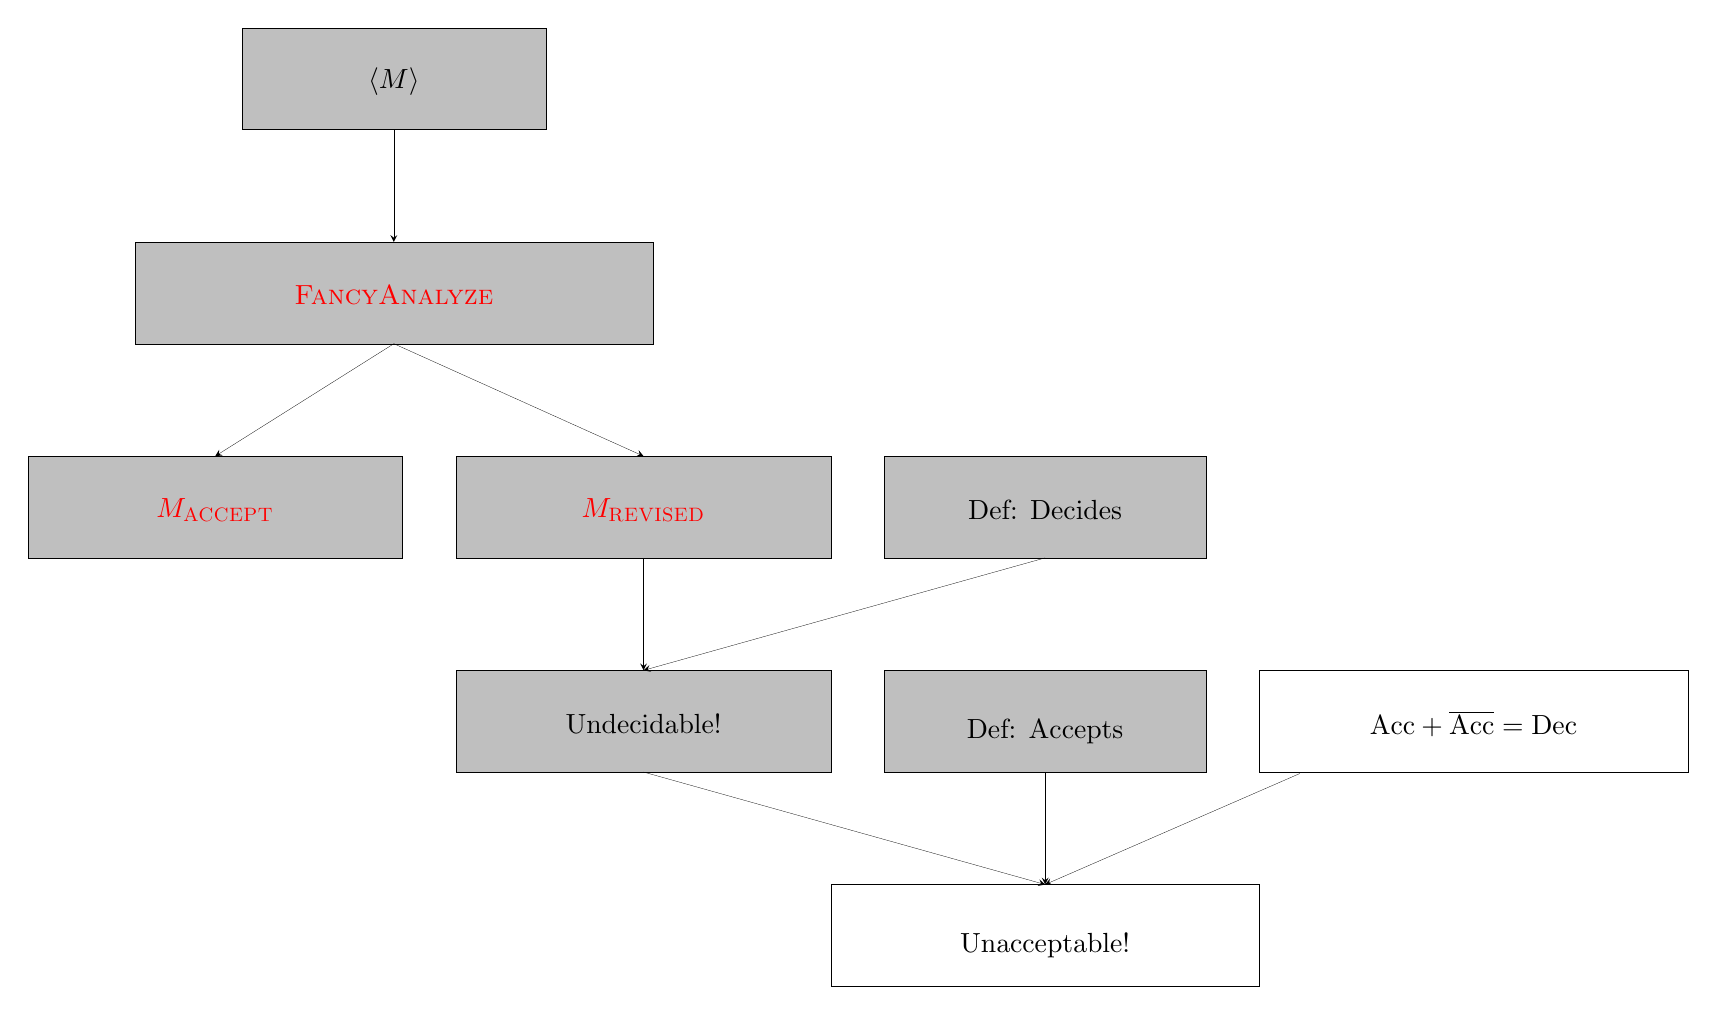
\begin{tikzpicture}
\pgftransformxscale{0.68000}
\pgftransformyscale{-0.680000}
\definecolor{dialinecolor}{rgb}{0.000000, 0.000000, 0.000000}
\pgfsetstrokecolor{dialinecolor}
\definecolor{dialinecolor}{rgb}{1.000000, 1.000000, 1.000000}
\pgfsetfillcolor{dialinecolor}
\definecolor{dialinecolor}{rgb}{1.000000, 1.000000, 1.000000}
\pgfsetfillcolor{black!25}
\fill (12.000000\du,9.000000\du)--(12.000000\du,10.900000\du)--(19.000000\du,10.900000\du)--(19.000000\du,9.000000\du)--cycle;
\pgfsetlinewidth{0.100000\du}
\pgfsetdash{}{0pt}
\pgfsetdash{}{0pt}
\pgfsetmiterjoin
\definecolor{dialinecolor}{rgb}{0.000000, 0.000000, 0.000000}
\pgfsetstrokecolor{dialinecolor}
\draw (12.000000\du,9.000000\du)--(12.000000\du,10.900000\du)--(19.000000\du,10.900000\du)--(19.000000\du,9.000000\du)--cycle;
% setfont left to latex
\definecolor{dialinecolor}{rgb}{0.000000, 0.000000, 0.000000}
\pgfsetstrokecolor{dialinecolor}
\node at (15.500000\du,10.000\du){\MACC};
\definecolor{dialinecolor}{rgb}{1.000000, 1.000000, 1.000000}
\pgfsetfillcolor{black!25}
\fill (20.000000\du,9.000000\du)--(20.000000\du,10.900000\du)--(27.000000\du,10.900000\du)--(27.000000\du,9.000000\du)--cycle;
\pgfsetlinewidth{0.100000\du}
\pgfsetdash{}{0pt}
\pgfsetdash{}{0pt}
\pgfsetmiterjoin
\definecolor{dialinecolor}{rgb}{0.000000, 0.000000, 0.000000}
\pgfsetstrokecolor{dialinecolor}
\draw (20.000000\du,9.000000\du)--(20.000000\du,10.900000\du)--(27.000000\du,10.900000\du)--(27.000000\du,9.000000\du)--cycle;
% setfont left to latex
\definecolor{dialinecolor}{rgb}{0.000000, 0.000000, 0.000000}
\pgfsetstrokecolor{dialinecolor}
\node at (23.500000\du,10.000\du){\MREV};
\definecolor{dialinecolor}{rgb}{1.000000, 1.000000, 1.000000}
\pgfsetfillcolor{dialinecolor}
\fill (35.000000\du,13.000000\du)--(35.000000\du,14.900000\du)--(41.000000\du,14.900000\du)--(41.000000\du,13.000000\du)--cycle;
\pgfsetlinewidth{0.100000\du}
\pgfsetdash{}{0pt}
\pgfsetdash{}{0pt}
\pgfsetmiterjoin
\definecolor{dialinecolor}{rgb}{0.000000, 0.000000, 0.000000}
\pgfsetstrokecolor{dialinecolor}
\draw (35.000000\du,13.000000\du)--(35.000000\du,14.900000\du)--(43.000000\du,14.900000\du)--(43.000000\du,13.000000\du)--cycle;
% setfont left to latex
\definecolor{dialinecolor}{rgb}{0.000000, 0.000000, 0.000000}
\pgfsetstrokecolor{dialinecolor}
\node at (39.000000\du,14.0000\du){$\text{Acc}+\overline{\text{Acc}}=\text{Dec}$};
\definecolor{dialinecolor}{rgb}{1.000000, 1.000000, 1.000000}
\pgfsetfillcolor{black!25}
\fill (14.000000\du,5.000000\du)--(14.000000\du,6.900000\du)--(23.672500\du,6.900000\du)--(23.672500\du,5.000000\du)--cycle;
\pgfsetlinewidth{0.100000\du}
\pgfsetdash{}{0pt}
\pgfsetdash{}{0pt}
\pgfsetmiterjoin
\definecolor{dialinecolor}{rgb}{0.000000, 0.000000, 0.000000}
\pgfsetstrokecolor{dialinecolor}
\draw (14.000000\du,5.000000\du)--(14.000000\du,6.900000\du)--(23.672500\du,6.900000\du)--(23.672500\du,5.000000\du)--cycle;
% setfont left to latex
\definecolor{dialinecolor}{rgb}{0.000000, 0.000000, 0.000000}
\pgfsetstrokecolor{dialinecolor}
\node at (18.836250\du,6.000\du){\func{FancyAnalyze}};
\definecolor{dialinecolor}{rgb}{1.000000, 1.000000, 1.000000}
\pgfsetfillcolor{dialinecolor}
\fill (28.000000\du,13.000000\du)--(28.000000\du,14.900000\du)--(34.000000\du,14.900000\du)--(34.000000\du,13.000000\du)--cycle;
\pgfsetlinewidth{0.100000\du}
\pgfsetdash{}{0pt}
\pgfsetdash{}{0pt}
\pgfsetmiterjoin
\definecolor{dialinecolor}{rgb}{0.000000, 0.000000, 0.000000}
\pgfsetstrokecolor{dialinecolor}
\pgfsetfillcolor{black!25}
\fill (16.000000\du,1.000000\du)--(16.000000\du,2.900000\du)--(21.672500\du,2.900000\du)--(21.672500\du,1.000000\du)--cycle;
\definecolor{dialinecolor}{rgb}{0.000000, 0.000000, 0.000000}\draw (16.000000\du,1.000000\du)--(16.000000\du,2.900000\du)--(21.672500\du,2.900000\du)--(21.672500\du,1.000000\du)--cycle;
% setfont left to latex
\definecolor{dialinecolor}{rgb}{0.000000, 0.000000, 0.000000}
\pgfsetstrokecolor{dialinecolor}
\node at (18.836250\du,2.000\du){\str{M}};
\definecolor{dialinecolor}{rgb}{1.000000, 1.000000, 1.000000}
\pgfsetfillcolor{black!25}
\fill (28.000000\du,13.000000\du)--(28.000000\du,14.900000\du)--(34.000000\du,14.900000\du)--(34.000000\du,13.000000\du)--cycle;
\pgfsetlinewidth{0.100000\du}
\pgfsetdash{}{0pt}
\pgfsetdash{}{0pt}
\pgfsetmiterjoin
\definecolor{dialinecolor}{rgb}{0.000000, 0.000000, 0.000000}
\pgfsetstrokecolor{dialinecolor}
\draw (28.000000\du,13.000000\du)--(28.000000\du,14.900000\du)--(34.000000\du,14.900000\du)--(34.000000\du,13.000000\du)--cycle;
% setfont left to latex
\definecolor{dialinecolor}{rgb}{0.000000, 0.000000, 0.000000}
\pgfsetstrokecolor{dialinecolor}
\node at (31.000000\du,14.145000\du){Def: Accepts};
\definecolor{dialinecolor}{rgb}{1.000000, 1.000000, 1.000000}
\pgfsetfillcolor{black!25}
\fill (28.000000\du,9.000000\du)--(28.000000\du,10.900000\du)--(34.000000\du,10.900000\du)--(34.000000\du,9.000000\du)--cycle;
\pgfsetlinewidth{0.100000\du}
\pgfsetdash{}{0pt}
\pgfsetdash{}{0pt}
\pgfsetmiterjoin
\definecolor{dialinecolor}{rgb}{0.000000, 0.000000, 0.000000}
\pgfsetstrokecolor{dialinecolor}
\draw (28.000000\du,9.000000\du)--(28.000000\du,10.900000\du)--(34.000000\du,10.900000\du)--(34.000000\du,9.000000\du)--cycle;
% setfont left to latex
\definecolor{dialinecolor}{rgb}{0.000000, 0.000000, 0.000000}
\pgfsetstrokecolor{dialinecolor}
\node at (31.000000\du,10.000\du){Def: Decides};
\definecolor{dialinecolor}{rgb}{1.000000, 1.000000, 1.000000}
\pgfsetfillcolor{black!25}
\fill (20.000000\du,13.000000\du)--(20.000000\du,14.900000\du)--(27.000000\du,14.900000\du)--(27.000000\du,13.000000\du)--cycle;
\pgfsetlinewidth{0.100000\du}
\pgfsetdash{}{0pt}
\pgfsetdash{}{0pt}
\pgfsetmiterjoin
\definecolor{dialinecolor}{rgb}{0.000000, 0.000000, 0.000000}
\pgfsetstrokecolor{dialinecolor}
\draw (20.000000\du,13.000000\du)--(20.000000\du,14.900000\du)--(27.000000\du,14.900000\du)--(27.000000\du,13.000000\du)--cycle;
% setfont left to latex
\definecolor{dialinecolor}{rgb}{0.000000, 0.000000, 0.000000}
\pgfsetstrokecolor{dialinecolor}
\node at (23.500000\du,14.000\du){Undecidable!};
\definecolor{dialinecolor}{rgb}{1.000000, 1.000000, 1.000000}
\pgfsetfillcolor{dialinecolor}
\fill (28.000000\du,17.000000\du)--(28.000000\du,18.900000\du)--(34.000000\du,18.900000\du)--(34.000000\du,17.000000\du)--cycle;
\pgfsetlinewidth{0.100000\du}
\pgfsetdash{}{0pt}
\pgfsetdash{}{0pt}
\pgfsetmiterjoin
\definecolor{dialinecolor}{rgb}{0.000000, 0.000000, 0.000000}
\pgfsetstrokecolor{dialinecolor}
\draw (27.000000\du,17.000000\du)--(27.000000\du,18.900000\du)--(35.000000\du,18.900000\du)--(35.000000\du,17.000000\du)--cycle;
% setfont left to latex
\definecolor{dialinecolor}{rgb}{0.000000, 0.000000, 0.000000}
\pgfsetstrokecolor{dialinecolor}
\node at (31.000000\du,18.145000\du){Unacceptable!};
\pgfsetlinewidth{0.100000\du}
\pgfsetdash{}{0pt}
\pgfsetdash{}{0pt}
\pgfsetbuttcap
{
\definecolor{dialinecolor}{rgb}{0.000000, 0.000000, 0.000000}
\pgfsetfillcolor{dialinecolor}
% was here!!!
\pgfsetarrowsend{stealth}
\definecolor{dialinecolor}{rgb}{0.000000, 0.000000, 0.000000}
\pgfsetstrokecolor{dialinecolor}
\draw (18.836250\du,2.900000\du)--(18.836250\du,5.000000\du);
}
\pgfsetlinewidth{0.100000\du}
\pgfsetdash{}{0pt}
\pgfsetdash{}{0pt}
\pgfsetbuttcap
{
\definecolor{dialinecolor}{rgb}{0.000000, 0.000000, 0.000000}
\pgfsetfillcolor{dialinecolor}
% was here!!!
\pgfsetarrowsend{stealth}
\definecolor{dialinecolor}{rgb}{0.000000, 0.000000, 0.000000}
\pgfsetstrokecolor{dialinecolor}
\draw (18.836250\du,6.900000\du)--(15.500000\du,9.000000\du);
}
\pgfsetlinewidth{0.100000\du}
\pgfsetdash{}{0pt}
\pgfsetdash{}{0pt}
\pgfsetbuttcap
{
\definecolor{dialinecolor}{rgb}{0.000000, 0.000000, 0.000000}
\pgfsetfillcolor{dialinecolor}
% was here!!!
\pgfsetarrowsend{stealth}
\definecolor{dialinecolor}{rgb}{0.000000, 0.000000, 0.000000}
\pgfsetstrokecolor{dialinecolor}
\draw (18.836250\du,6.900000\du)--(23.500000\du,9.000000\du);
}
\pgfsetlinewidth{0.100000\du}
\pgfsetdash{}{0pt}
\pgfsetdash{}{0pt}
\pgfsetbuttcap
{
\definecolor{dialinecolor}{rgb}{0.000000, 0.000000, 0.000000}
\pgfsetfillcolor{dialinecolor}
% was here!!!
\pgfsetarrowsend{stealth}
\definecolor{dialinecolor}{rgb}{0.000000, 0.000000, 0.000000}
\pgfsetstrokecolor{dialinecolor}
\draw (23.500000\du,10.900000\du)--(23.500000\du,13.000000\du);
}
\pgfsetlinewidth{0.100000\du}
\pgfsetdash{}{0pt}
\pgfsetdash{}{0pt}
\pgfsetbuttcap
{
\definecolor{dialinecolor}{rgb}{0.000000, 0.000000, 0.000000}
\pgfsetfillcolor{dialinecolor}
% was here!!!
\pgfsetarrowsend{stealth}
\definecolor{dialinecolor}{rgb}{0.000000, 0.000000, 0.000000}
\pgfsetstrokecolor{dialinecolor}
\draw (31.000000\du,10.900000\du)--(23.500000\du,13.000000\du);
}
\pgfsetlinewidth{0.100000\du}
\pgfsetdash{}{0pt}
\pgfsetdash{}{0pt}
\pgfsetbuttcap
{
\definecolor{dialinecolor}{rgb}{0.000000, 0.000000, 0.000000}
\pgfsetfillcolor{dialinecolor}
% was here!!!
\pgfsetarrowsend{stealth}
\definecolor{dialinecolor}{rgb}{0.000000, 0.000000, 0.000000}
\pgfsetstrokecolor{dialinecolor}
\draw (23.500000\du,14.900000\du)--(31.000000\du,17.000000\du);
}
\pgfsetlinewidth{0.100000\du}
\pgfsetdash{}{0pt}
\pgfsetdash{}{0pt}
\pgfsetbuttcap
{
\definecolor{dialinecolor}{rgb}{0.000000, 0.000000, 0.000000}
\pgfsetfillcolor{dialinecolor}
% was here!!!
\pgfsetarrowsend{stealth}
\definecolor{dialinecolor}{rgb}{0.000000, 0.000000, 0.000000}
\pgfsetstrokecolor{dialinecolor}
\draw (31.000000\du,14.900000\du)--(31.000000\du,17.000000\du);
}
\pgfsetlinewidth{0.100000\du}
\pgfsetdash{}{0pt}
\pgfsetdash{}{0pt}
\pgfsetbuttcap
{
\definecolor{dialinecolor}{rgb}{0.000000, 0.000000, 0.000000}
\pgfsetfillcolor{dialinecolor}
% was here!!!
\pgfsetarrowsend{stealth}
\definecolor{dialinecolor}{rgb}{0.000000, 0.000000, 0.000000}
\pgfsetstrokecolor{dialinecolor}
\draw (35.757813\du,14.926953\du)--(31.000000\du,17.000000\du);
}
\end{tikzpicture}
}

\end{frame}

\begin{frame}{$\text{Acc}+\overline{\text{Acc}}=\text{Dec}$}

  foobar

\end{frame}

\begin{frame}{The Plan}

  % Graphic for TeX using PGF
% Title: C:\Users\Joshua\Documents\teaching\csueb-guest-teaching\flow-diagram.dia
% Creator: Dia v0.97.2
% CreationDate: Tue Feb 04 08:43:25 2014
% For: Joshua
% \usepackage{tikz}
% The following commands are not supported in PSTricks at present
% We define them conditionally, so when they are implemented,
% this pgf file will use them.
\ifx\du\undefined
  \newlength{\du}
\fi
\setlength{\du}{15\unitlength}
{\footnotesize
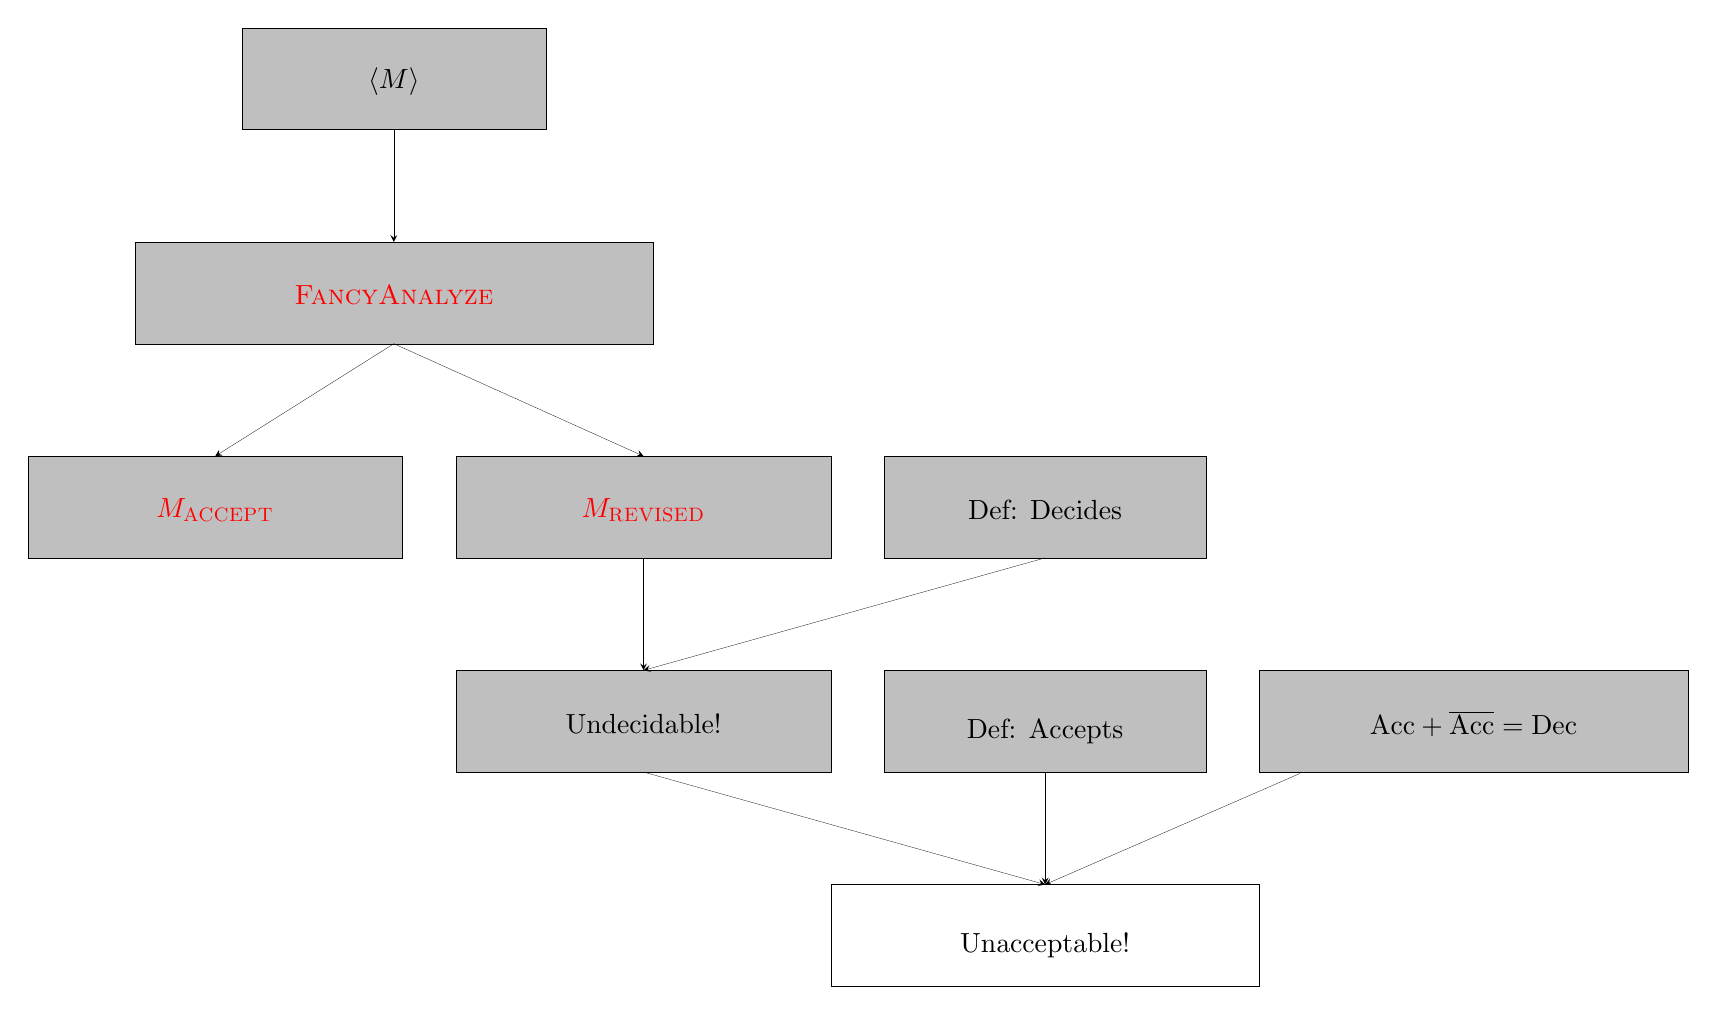
\begin{tikzpicture}
\pgftransformxscale{0.68000}
\pgftransformyscale{-0.680000}
\definecolor{dialinecolor}{rgb}{0.000000, 0.000000, 0.000000}
\pgfsetstrokecolor{dialinecolor}
\definecolor{dialinecolor}{rgb}{1.000000, 1.000000, 1.000000}
\pgfsetfillcolor{dialinecolor}
\definecolor{dialinecolor}{rgb}{1.000000, 1.000000, 1.000000}
\pgfsetfillcolor{black!25}
\fill (12.000000\du,9.000000\du)--(12.000000\du,10.900000\du)--(19.000000\du,10.900000\du)--(19.000000\du,9.000000\du)--cycle;
\pgfsetlinewidth{0.100000\du}
\pgfsetdash{}{0pt}
\pgfsetdash{}{0pt}
\pgfsetmiterjoin
\definecolor{dialinecolor}{rgb}{0.000000, 0.000000, 0.000000}
\pgfsetstrokecolor{dialinecolor}
\draw (12.000000\du,9.000000\du)--(12.000000\du,10.900000\du)--(19.000000\du,10.900000\du)--(19.000000\du,9.000000\du)--cycle;
% setfont left to latex
\definecolor{dialinecolor}{rgb}{0.000000, 0.000000, 0.000000}
\pgfsetstrokecolor{dialinecolor}
\node at (15.500000\du,10.000\du){\MACC};
\definecolor{dialinecolor}{rgb}{1.000000, 1.000000, 1.000000}
\pgfsetfillcolor{black!25}
\fill (20.000000\du,9.000000\du)--(20.000000\du,10.900000\du)--(27.000000\du,10.900000\du)--(27.000000\du,9.000000\du)--cycle;
\pgfsetlinewidth{0.100000\du}
\pgfsetdash{}{0pt}
\pgfsetdash{}{0pt}
\pgfsetmiterjoin
\definecolor{dialinecolor}{rgb}{0.000000, 0.000000, 0.000000}
\pgfsetstrokecolor{dialinecolor}
\draw (20.000000\du,9.000000\du)--(20.000000\du,10.900000\du)--(27.000000\du,10.900000\du)--(27.000000\du,9.000000\du)--cycle;
% setfont left to latex
\definecolor{dialinecolor}{rgb}{0.000000, 0.000000, 0.000000}
\pgfsetstrokecolor{dialinecolor}
\node at (23.500000\du,10.000\du){\MREV};
\definecolor{dialinecolor}{rgb}{1.000000, 1.000000, 1.000000}
\pgfsetfillcolor{black!25}
\fill (35.000000\du,13.000000\du)--(35.000000\du,14.900000\du)--(43.000000\du,14.900000\du)--(43.000000\du,13.000000\du)--cycle;
\pgfsetlinewidth{0.100000\du}
\pgfsetdash{}{0pt}
\pgfsetdash{}{0pt}
\pgfsetmiterjoin
\definecolor{dialinecolor}{rgb}{0.000000, 0.000000, 0.000000}
\pgfsetstrokecolor{dialinecolor}
\draw (35.000000\du,13.000000\du)--(35.000000\du,14.900000\du)--(43.000000\du,14.900000\du)--(43.000000\du,13.000000\du)--cycle;
% setfont left to latex
\definecolor{dialinecolor}{rgb}{0.000000, 0.000000, 0.000000}
\pgfsetstrokecolor{dialinecolor}
\node at (39.000000\du,14.0000\du){$\text{Acc}+\overline{\text{Acc}}=\text{Dec}$};
\definecolor{dialinecolor}{rgb}{1.000000, 1.000000, 1.000000}
\pgfsetfillcolor{black!25}
\fill (14.000000\du,5.000000\du)--(14.000000\du,6.900000\du)--(23.672500\du,6.900000\du)--(23.672500\du,5.000000\du)--cycle;
\pgfsetlinewidth{0.100000\du}
\pgfsetdash{}{0pt}
\pgfsetdash{}{0pt}
\pgfsetmiterjoin
\definecolor{dialinecolor}{rgb}{0.000000, 0.000000, 0.000000}
\pgfsetstrokecolor{dialinecolor}
\draw (14.000000\du,5.000000\du)--(14.000000\du,6.900000\du)--(23.672500\du,6.900000\du)--(23.672500\du,5.000000\du)--cycle;
% setfont left to latex
\definecolor{dialinecolor}{rgb}{0.000000, 0.000000, 0.000000}
\pgfsetstrokecolor{dialinecolor}
\node at (18.836250\du,6.000\du){\func{FancyAnalyze}};
\definecolor{dialinecolor}{rgb}{1.000000, 1.000000, 1.000000}
\pgfsetfillcolor{dialinecolor}
\fill (28.000000\du,13.000000\du)--(28.000000\du,14.900000\du)--(34.000000\du,14.900000\du)--(34.000000\du,13.000000\du)--cycle;
\pgfsetlinewidth{0.100000\du}
\pgfsetdash{}{0pt}
\pgfsetdash{}{0pt}
\pgfsetmiterjoin
\definecolor{dialinecolor}{rgb}{0.000000, 0.000000, 0.000000}
\pgfsetstrokecolor{dialinecolor}
\pgfsetfillcolor{black!25}
\fill (16.000000\du,1.000000\du)--(16.000000\du,2.900000\du)--(21.672500\du,2.900000\du)--(21.672500\du,1.000000\du)--cycle;
\definecolor{dialinecolor}{rgb}{0.000000, 0.000000, 0.000000}\draw (16.000000\du,1.000000\du)--(16.000000\du,2.900000\du)--(21.672500\du,2.900000\du)--(21.672500\du,1.000000\du)--cycle;
% setfont left to latex
\definecolor{dialinecolor}{rgb}{0.000000, 0.000000, 0.000000}
\pgfsetstrokecolor{dialinecolor}
\node at (18.836250\du,2.000\du){\str{M}};
\definecolor{dialinecolor}{rgb}{1.000000, 1.000000, 1.000000}
\pgfsetfillcolor{black!25}
\fill (28.000000\du,13.000000\du)--(28.000000\du,14.900000\du)--(34.000000\du,14.900000\du)--(34.000000\du,13.000000\du)--cycle;
\pgfsetlinewidth{0.100000\du}
\pgfsetdash{}{0pt}
\pgfsetdash{}{0pt}
\pgfsetmiterjoin
\definecolor{dialinecolor}{rgb}{0.000000, 0.000000, 0.000000}
\pgfsetstrokecolor{dialinecolor}
\draw (28.000000\du,13.000000\du)--(28.000000\du,14.900000\du)--(34.000000\du,14.900000\du)--(34.000000\du,13.000000\du)--cycle;
% setfont left to latex
\definecolor{dialinecolor}{rgb}{0.000000, 0.000000, 0.000000}
\pgfsetstrokecolor{dialinecolor}
\node at (31.000000\du,14.145000\du){Def: Accepts};
\definecolor{dialinecolor}{rgb}{1.000000, 1.000000, 1.000000}
\pgfsetfillcolor{black!25}
\fill (28.000000\du,9.000000\du)--(28.000000\du,10.900000\du)--(34.000000\du,10.900000\du)--(34.000000\du,9.000000\du)--cycle;
\pgfsetlinewidth{0.100000\du}
\pgfsetdash{}{0pt}
\pgfsetdash{}{0pt}
\pgfsetmiterjoin
\definecolor{dialinecolor}{rgb}{0.000000, 0.000000, 0.000000}
\pgfsetstrokecolor{dialinecolor}
\draw (28.000000\du,9.000000\du)--(28.000000\du,10.900000\du)--(34.000000\du,10.900000\du)--(34.000000\du,9.000000\du)--cycle;
% setfont left to latex
\definecolor{dialinecolor}{rgb}{0.000000, 0.000000, 0.000000}
\pgfsetstrokecolor{dialinecolor}
\node at (31.000000\du,10.000\du){Def: Decides};
\definecolor{dialinecolor}{rgb}{1.000000, 1.000000, 1.000000}
\pgfsetfillcolor{black!25}
\fill (20.000000\du,13.000000\du)--(20.000000\du,14.900000\du)--(27.000000\du,14.900000\du)--(27.000000\du,13.000000\du)--cycle;
\pgfsetlinewidth{0.100000\du}
\pgfsetdash{}{0pt}
\pgfsetdash{}{0pt}
\pgfsetmiterjoin
\definecolor{dialinecolor}{rgb}{0.000000, 0.000000, 0.000000}
\pgfsetstrokecolor{dialinecolor}
\draw (20.000000\du,13.000000\du)--(20.000000\du,14.900000\du)--(27.000000\du,14.900000\du)--(27.000000\du,13.000000\du)--cycle;
% setfont left to latex
\definecolor{dialinecolor}{rgb}{0.000000, 0.000000, 0.000000}
\pgfsetstrokecolor{dialinecolor}
\node at (23.500000\du,14.000\du){Undecidable!};
\definecolor{dialinecolor}{rgb}{1.000000, 1.000000, 1.000000}
\pgfsetfillcolor{dialinecolor}
\fill (28.000000\du,17.000000\du)--(28.000000\du,18.900000\du)--(34.000000\du,18.900000\du)--(34.000000\du,17.000000\du)--cycle;
\pgfsetlinewidth{0.100000\du}
\pgfsetdash{}{0pt}
\pgfsetdash{}{0pt}
\pgfsetmiterjoin
\definecolor{dialinecolor}{rgb}{0.000000, 0.000000, 0.000000}
\pgfsetstrokecolor{dialinecolor}
\draw (27.000000\du,17.000000\du)--(27.000000\du,18.900000\du)--(35.000000\du,18.900000\du)--(35.000000\du,17.000000\du)--cycle;
% setfont left to latex
\definecolor{dialinecolor}{rgb}{0.000000, 0.000000, 0.000000}
\pgfsetstrokecolor{dialinecolor}
\node at (31.000000\du,18.145000\du){Unacceptable!};
\pgfsetlinewidth{0.100000\du}
\pgfsetdash{}{0pt}
\pgfsetdash{}{0pt}
\pgfsetbuttcap
{
\definecolor{dialinecolor}{rgb}{0.000000, 0.000000, 0.000000}
\pgfsetfillcolor{dialinecolor}
% was here!!!
\pgfsetarrowsend{stealth}
\definecolor{dialinecolor}{rgb}{0.000000, 0.000000, 0.000000}
\pgfsetstrokecolor{dialinecolor}
\draw (18.836250\du,2.900000\du)--(18.836250\du,5.000000\du);
}
\pgfsetlinewidth{0.100000\du}
\pgfsetdash{}{0pt}
\pgfsetdash{}{0pt}
\pgfsetbuttcap
{
\definecolor{dialinecolor}{rgb}{0.000000, 0.000000, 0.000000}
\pgfsetfillcolor{dialinecolor}
% was here!!!
\pgfsetarrowsend{stealth}
\definecolor{dialinecolor}{rgb}{0.000000, 0.000000, 0.000000}
\pgfsetstrokecolor{dialinecolor}
\draw (18.836250\du,6.900000\du)--(15.500000\du,9.000000\du);
}
\pgfsetlinewidth{0.100000\du}
\pgfsetdash{}{0pt}
\pgfsetdash{}{0pt}
\pgfsetbuttcap
{
\definecolor{dialinecolor}{rgb}{0.000000, 0.000000, 0.000000}
\pgfsetfillcolor{dialinecolor}
% was here!!!
\pgfsetarrowsend{stealth}
\definecolor{dialinecolor}{rgb}{0.000000, 0.000000, 0.000000}
\pgfsetstrokecolor{dialinecolor}
\draw (18.836250\du,6.900000\du)--(23.500000\du,9.000000\du);
}
\pgfsetlinewidth{0.100000\du}
\pgfsetdash{}{0pt}
\pgfsetdash{}{0pt}
\pgfsetbuttcap
{
\definecolor{dialinecolor}{rgb}{0.000000, 0.000000, 0.000000}
\pgfsetfillcolor{dialinecolor}
% was here!!!
\pgfsetarrowsend{stealth}
\definecolor{dialinecolor}{rgb}{0.000000, 0.000000, 0.000000}
\pgfsetstrokecolor{dialinecolor}
\draw (23.500000\du,10.900000\du)--(23.500000\du,13.000000\du);
}
\pgfsetlinewidth{0.100000\du}
\pgfsetdash{}{0pt}
\pgfsetdash{}{0pt}
\pgfsetbuttcap
{
\definecolor{dialinecolor}{rgb}{0.000000, 0.000000, 0.000000}
\pgfsetfillcolor{dialinecolor}
% was here!!!
\pgfsetarrowsend{stealth}
\definecolor{dialinecolor}{rgb}{0.000000, 0.000000, 0.000000}
\pgfsetstrokecolor{dialinecolor}
\draw (31.000000\du,10.900000\du)--(23.500000\du,13.000000\du);
}
\pgfsetlinewidth{0.100000\du}
\pgfsetdash{}{0pt}
\pgfsetdash{}{0pt}
\pgfsetbuttcap
{
\definecolor{dialinecolor}{rgb}{0.000000, 0.000000, 0.000000}
\pgfsetfillcolor{dialinecolor}
% was here!!!
\pgfsetarrowsend{stealth}
\definecolor{dialinecolor}{rgb}{0.000000, 0.000000, 0.000000}
\pgfsetstrokecolor{dialinecolor}
\draw (23.500000\du,14.900000\du)--(31.000000\du,17.000000\du);
}
\pgfsetlinewidth{0.100000\du}
\pgfsetdash{}{0pt}
\pgfsetdash{}{0pt}
\pgfsetbuttcap
{
\definecolor{dialinecolor}{rgb}{0.000000, 0.000000, 0.000000}
\pgfsetfillcolor{dialinecolor}
% was here!!!
\pgfsetarrowsend{stealth}
\definecolor{dialinecolor}{rgb}{0.000000, 0.000000, 0.000000}
\pgfsetstrokecolor{dialinecolor}
\draw (31.000000\du,14.900000\du)--(31.000000\du,17.000000\du);
}
\pgfsetlinewidth{0.100000\du}
\pgfsetdash{}{0pt}
\pgfsetdash{}{0pt}
\pgfsetbuttcap
{
\definecolor{dialinecolor}{rgb}{0.000000, 0.000000, 0.000000}
\pgfsetfillcolor{dialinecolor}
% was here!!!
\pgfsetarrowsend{stealth}
\definecolor{dialinecolor}{rgb}{0.000000, 0.000000, 0.000000}
\pgfsetstrokecolor{dialinecolor}
\draw (35.757813\du,14.926953\du)--(31.000000\du,17.000000\du);
}
\end{tikzpicture}
}

\end{frame}

\begin{frame}{Unacceptable!}

  We can also prove there exists a language that cannot be accepted
  (recognized).

  \vskip 0.25in

  It's simply,

  \begin{equation*}
    \overline{\text{ACCEPT}_{\text{TM}}} = \{ (\langle M \rangle, w) : M \text{
      does not accept } w\}.
  \end{equation*}

\end{frame}

\begin{frame}{Unacceptable!}

  $\overline{\text{ACCEPT}_{\text{TM}}}$ is unacceptable.

  \vskip 0.25in

  Proof: Suppose it is acceptable. Then,

  \begin{itemize}

  \item $\overline{\text{ACCEPT}_{\text{TM}}}$ would be acceptable (by
    supposition).

  \item $\text{ACCEPT}_{\text{TM}}$ is acceptable (proved earlier).

  \item So, $\text{ACCEPT}_{\text{TM}}$ is decidable! Impossible (proved earlier).

  \end{itemize}

  So $\overline{\text{ACCEPT}_{\text{TM}}}$ is not acceptable.

\end{frame}

\begin{frame}{The Plan}

  % Graphic for TeX using PGF
% Title: C:\Users\Joshua\Documents\teaching\csueb-guest-teaching\flow-diagram.dia
% Creator: Dia v0.97.2
% CreationDate: Tue Feb 04 08:43:25 2014
% For: Joshua
% \usepackage{tikz}
% The following commands are not supported in PSTricks at present
% We define them conditionally, so when they are implemented,
% this pgf file will use them.
\ifx\du\undefined
  \newlength{\du}
\fi
\setlength{\du}{15\unitlength}
{\footnotesize
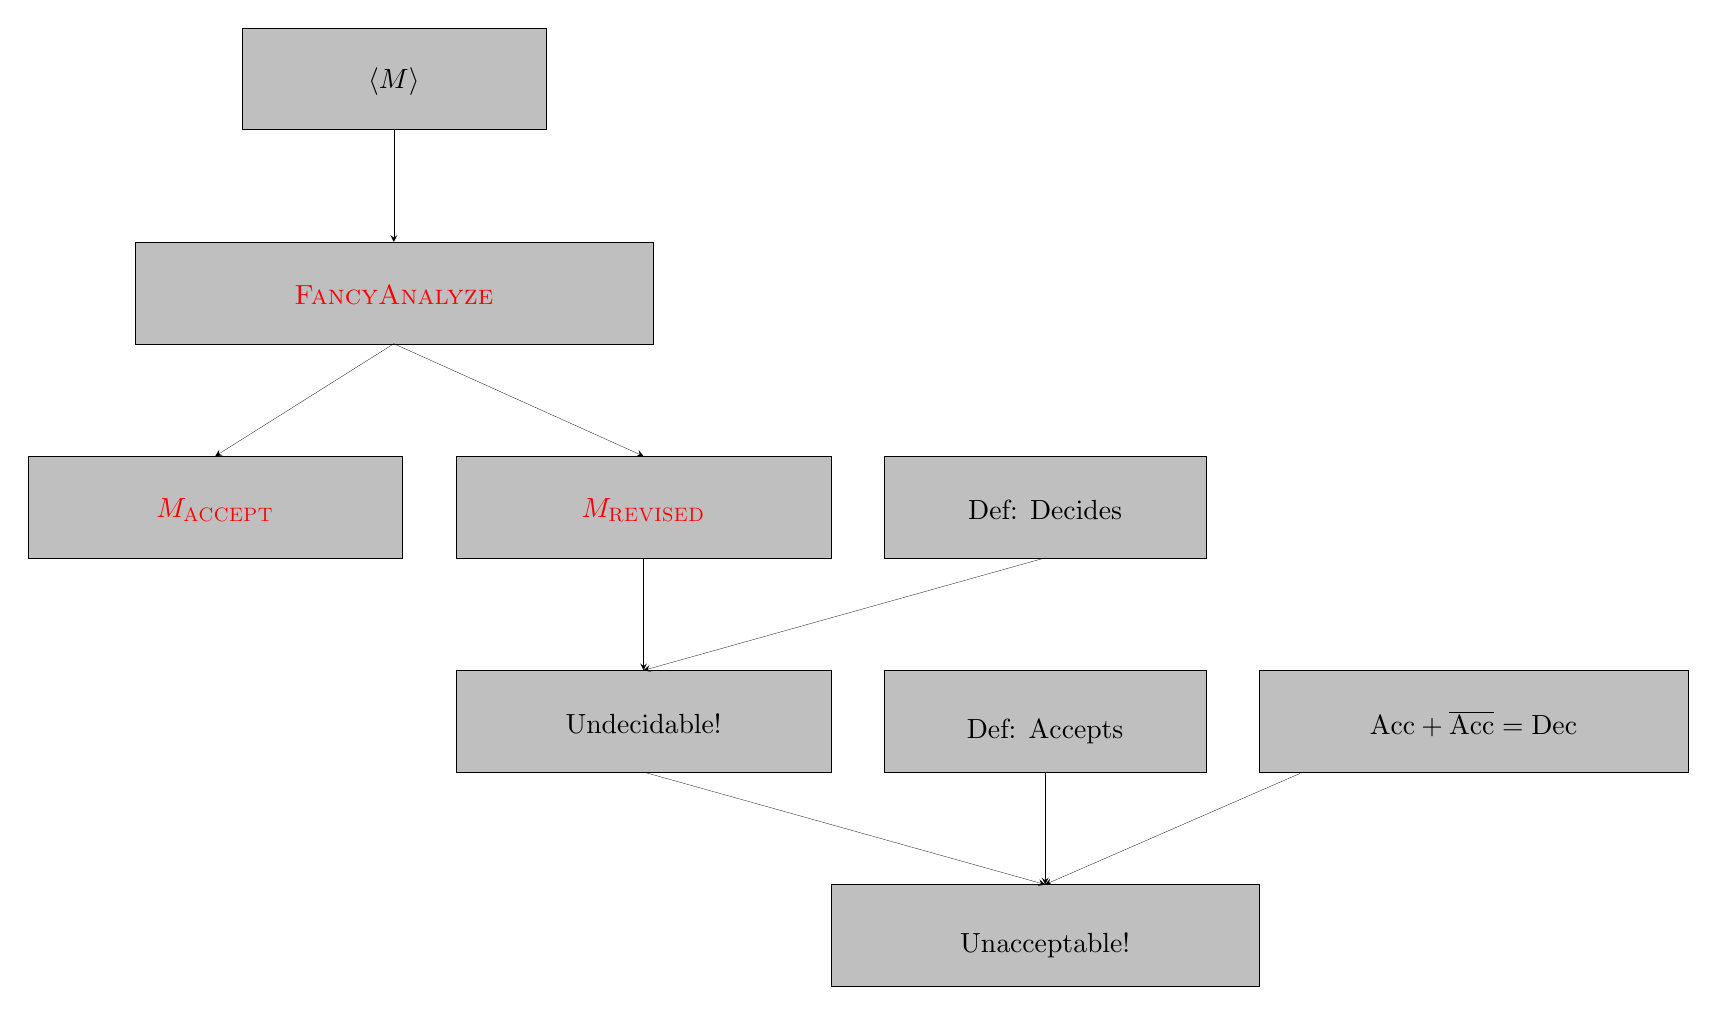
\begin{tikzpicture}
\pgftransformxscale{0.68000}
\pgftransformyscale{-0.680000}
\definecolor{dialinecolor}{rgb}{0.000000, 0.000000, 0.000000}
\pgfsetstrokecolor{dialinecolor}
\definecolor{dialinecolor}{rgb}{1.000000, 1.000000, 1.000000}
\pgfsetfillcolor{dialinecolor}
\definecolor{dialinecolor}{rgb}{1.000000, 1.000000, 1.000000}
\pgfsetfillcolor{black!25}
\fill (12.000000\du,9.000000\du)--(12.000000\du,10.900000\du)--(19.000000\du,10.900000\du)--(19.000000\du,9.000000\du)--cycle;
\pgfsetlinewidth{0.100000\du}
\pgfsetdash{}{0pt}
\pgfsetdash{}{0pt}
\pgfsetmiterjoin
\definecolor{dialinecolor}{rgb}{0.000000, 0.000000, 0.000000}
\pgfsetstrokecolor{dialinecolor}
\draw (12.000000\du,9.000000\du)--(12.000000\du,10.900000\du)--(19.000000\du,10.900000\du)--(19.000000\du,9.000000\du)--cycle;
% setfont left to latex
\definecolor{dialinecolor}{rgb}{0.000000, 0.000000, 0.000000}
\pgfsetstrokecolor{dialinecolor}
\node at (15.500000\du,10.000\du){\MACC};
\definecolor{dialinecolor}{rgb}{1.000000, 1.000000, 1.000000}
\pgfsetfillcolor{black!25}
\fill (20.000000\du,9.000000\du)--(20.000000\du,10.900000\du)--(27.000000\du,10.900000\du)--(27.000000\du,9.000000\du)--cycle;
\pgfsetlinewidth{0.100000\du}
\pgfsetdash{}{0pt}
\pgfsetdash{}{0pt}
\pgfsetmiterjoin
\definecolor{dialinecolor}{rgb}{0.000000, 0.000000, 0.000000}
\pgfsetstrokecolor{dialinecolor}
\draw (20.000000\du,9.000000\du)--(20.000000\du,10.900000\du)--(27.000000\du,10.900000\du)--(27.000000\du,9.000000\du)--cycle;
% setfont left to latex
\definecolor{dialinecolor}{rgb}{0.000000, 0.000000, 0.000000}
\pgfsetstrokecolor{dialinecolor}
\node at (23.500000\du,10.000\du){\MREV};
\definecolor{dialinecolor}{rgb}{1.000000, 1.000000, 1.000000}
\pgfsetfillcolor{black!25}
\fill (35.000000\du,13.000000\du)--(35.000000\du,14.900000\du)--(43.000000\du,14.900000\du)--(43.000000\du,13.000000\du)--cycle;
\pgfsetlinewidth{0.100000\du}
\pgfsetdash{}{0pt}
\pgfsetdash{}{0pt}
\pgfsetmiterjoin
\definecolor{dialinecolor}{rgb}{0.000000, 0.000000, 0.000000}
\pgfsetstrokecolor{dialinecolor}
\draw (35.000000\du,13.000000\du)--(35.000000\du,14.900000\du)--(43.000000\du,14.900000\du)--(43.000000\du,13.000000\du)--cycle;
% setfont left to latex
\definecolor{dialinecolor}{rgb}{0.000000, 0.000000, 0.000000}
\pgfsetstrokecolor{dialinecolor}
\node at (39.000000\du,14.0000\du){$\text{Acc}+\overline{\text{Acc}}=\text{Dec}$};
\definecolor{dialinecolor}{rgb}{1.000000, 1.000000, 1.000000}
\pgfsetfillcolor{black!25}
\fill (14.000000\du,5.000000\du)--(14.000000\du,6.900000\du)--(23.672500\du,6.900000\du)--(23.672500\du,5.000000\du)--cycle;
\pgfsetlinewidth{0.100000\du}
\pgfsetdash{}{0pt}
\pgfsetdash{}{0pt}
\pgfsetmiterjoin
\definecolor{dialinecolor}{rgb}{0.000000, 0.000000, 0.000000}
\pgfsetstrokecolor{dialinecolor}
\draw (14.000000\du,5.000000\du)--(14.000000\du,6.900000\du)--(23.672500\du,6.900000\du)--(23.672500\du,5.000000\du)--cycle;
% setfont left to latex
\definecolor{dialinecolor}{rgb}{0.000000, 0.000000, 0.000000}
\pgfsetstrokecolor{dialinecolor}
\node at (18.836250\du,6.000\du){\func{FancyAnalyze}};
\definecolor{dialinecolor}{rgb}{1.000000, 1.000000, 1.000000}
\pgfsetfillcolor{dialinecolor}
\fill (28.000000\du,13.000000\du)--(28.000000\du,14.900000\du)--(34.000000\du,14.900000\du)--(34.000000\du,13.000000\du)--cycle;
\pgfsetlinewidth{0.100000\du}
\pgfsetdash{}{0pt}
\pgfsetdash{}{0pt}
\pgfsetmiterjoin
\definecolor{dialinecolor}{rgb}{0.000000, 0.000000, 0.000000}
\pgfsetstrokecolor{dialinecolor}
\pgfsetfillcolor{black!25}
\fill (16.000000\du,1.000000\du)--(16.000000\du,2.900000\du)--(21.672500\du,2.900000\du)--(21.672500\du,1.000000\du)--cycle;
\definecolor{dialinecolor}{rgb}{0.000000, 0.000000, 0.000000}\draw (16.000000\du,1.000000\du)--(16.000000\du,2.900000\du)--(21.672500\du,2.900000\du)--(21.672500\du,1.000000\du)--cycle;
% setfont left to latex
\definecolor{dialinecolor}{rgb}{0.000000, 0.000000, 0.000000}
\pgfsetstrokecolor{dialinecolor}
\node at (18.836250\du,2.000\du){\str{M}};
\definecolor{dialinecolor}{rgb}{1.000000, 1.000000, 1.000000}
\pgfsetfillcolor{black!25}
\fill (28.000000\du,13.000000\du)--(28.000000\du,14.900000\du)--(34.000000\du,14.900000\du)--(34.000000\du,13.000000\du)--cycle;
\pgfsetlinewidth{0.100000\du}
\pgfsetdash{}{0pt}
\pgfsetdash{}{0pt}
\pgfsetmiterjoin
\definecolor{dialinecolor}{rgb}{0.000000, 0.000000, 0.000000}
\pgfsetstrokecolor{dialinecolor}
\draw (28.000000\du,13.000000\du)--(28.000000\du,14.900000\du)--(34.000000\du,14.900000\du)--(34.000000\du,13.000000\du)--cycle;
% setfont left to latex
\definecolor{dialinecolor}{rgb}{0.000000, 0.000000, 0.000000}
\pgfsetstrokecolor{dialinecolor}
\node at (31.000000\du,14.145000\du){Def: Accepts};
\definecolor{dialinecolor}{rgb}{1.000000, 1.000000, 1.000000}
\pgfsetfillcolor{black!25}
\fill (28.000000\du,9.000000\du)--(28.000000\du,10.900000\du)--(34.000000\du,10.900000\du)--(34.000000\du,9.000000\du)--cycle;
\pgfsetlinewidth{0.100000\du}
\pgfsetdash{}{0pt}
\pgfsetdash{}{0pt}
\pgfsetmiterjoin
\definecolor{dialinecolor}{rgb}{0.000000, 0.000000, 0.000000}
\pgfsetstrokecolor{dialinecolor}
\draw (28.000000\du,9.000000\du)--(28.000000\du,10.900000\du)--(34.000000\du,10.900000\du)--(34.000000\du,9.000000\du)--cycle;
% setfont left to latex
\definecolor{dialinecolor}{rgb}{0.000000, 0.000000, 0.000000}
\pgfsetstrokecolor{dialinecolor}
\node at (31.000000\du,10.000\du){Def: Decides};
\definecolor{dialinecolor}{rgb}{1.000000, 1.000000, 1.000000}
\pgfsetfillcolor{black!25}
\fill (20.000000\du,13.000000\du)--(20.000000\du,14.900000\du)--(27.000000\du,14.900000\du)--(27.000000\du,13.000000\du)--cycle;
\pgfsetlinewidth{0.100000\du}
\pgfsetdash{}{0pt}
\pgfsetdash{}{0pt}
\pgfsetmiterjoin
\definecolor{dialinecolor}{rgb}{0.000000, 0.000000, 0.000000}
\pgfsetstrokecolor{dialinecolor}
\draw (20.000000\du,13.000000\du)--(20.000000\du,14.900000\du)--(27.000000\du,14.900000\du)--(27.000000\du,13.000000\du)--cycle;
% setfont left to latex
\definecolor{dialinecolor}{rgb}{0.000000, 0.000000, 0.000000}
\pgfsetstrokecolor{dialinecolor}
\node at (23.500000\du,14.000\du){Undecidable!};
\definecolor{dialinecolor}{rgb}{1.000000, 1.000000, 1.000000}
\pgfsetfillcolor{black!25}
\fill (27.000000\du,17.000000\du)--(27.000000\du,18.900000\du)--(35.000000\du,18.900000\du)--(35.000000\du,17.000000\du)--cycle;
\pgfsetlinewidth{0.100000\du}
\pgfsetdash{}{0pt}
\pgfsetdash{}{0pt}
\pgfsetmiterjoin
\definecolor{dialinecolor}{rgb}{0.000000, 0.000000, 0.000000}
\pgfsetstrokecolor{dialinecolor}
\draw (27.000000\du,17.000000\du)--(27.000000\du,18.900000\du)--(35.000000\du,18.900000\du)--(35.000000\du,17.000000\du)--cycle;
% setfont left to latex
\definecolor{dialinecolor}{rgb}{0.000000, 0.000000, 0.000000}
\pgfsetstrokecolor{dialinecolor}
\node at (31.000000\du,18.145000\du){Unacceptable!};
\pgfsetlinewidth{0.100000\du}
\pgfsetdash{}{0pt}
\pgfsetdash{}{0pt}
\pgfsetbuttcap
{
\definecolor{dialinecolor}{rgb}{0.000000, 0.000000, 0.000000}
\pgfsetfillcolor{dialinecolor}
% was here!!!
\pgfsetarrowsend{stealth}
\definecolor{dialinecolor}{rgb}{0.000000, 0.000000, 0.000000}
\pgfsetstrokecolor{dialinecolor}
\draw (18.836250\du,2.900000\du)--(18.836250\du,5.000000\du);
}
\pgfsetlinewidth{0.100000\du}
\pgfsetdash{}{0pt}
\pgfsetdash{}{0pt}
\pgfsetbuttcap
{
\definecolor{dialinecolor}{rgb}{0.000000, 0.000000, 0.000000}
\pgfsetfillcolor{dialinecolor}
% was here!!!
\pgfsetarrowsend{stealth}
\definecolor{dialinecolor}{rgb}{0.000000, 0.000000, 0.000000}
\pgfsetstrokecolor{dialinecolor}
\draw (18.836250\du,6.900000\du)--(15.500000\du,9.000000\du);
}
\pgfsetlinewidth{0.100000\du}
\pgfsetdash{}{0pt}
\pgfsetdash{}{0pt}
\pgfsetbuttcap
{
\definecolor{dialinecolor}{rgb}{0.000000, 0.000000, 0.000000}
\pgfsetfillcolor{dialinecolor}
% was here!!!
\pgfsetarrowsend{stealth}
\definecolor{dialinecolor}{rgb}{0.000000, 0.000000, 0.000000}
\pgfsetstrokecolor{dialinecolor}
\draw (18.836250\du,6.900000\du)--(23.500000\du,9.000000\du);
}
\pgfsetlinewidth{0.100000\du}
\pgfsetdash{}{0pt}
\pgfsetdash{}{0pt}
\pgfsetbuttcap
{
\definecolor{dialinecolor}{rgb}{0.000000, 0.000000, 0.000000}
\pgfsetfillcolor{dialinecolor}
% was here!!!
\pgfsetarrowsend{stealth}
\definecolor{dialinecolor}{rgb}{0.000000, 0.000000, 0.000000}
\pgfsetstrokecolor{dialinecolor}
\draw (23.500000\du,10.900000\du)--(23.500000\du,13.000000\du);
}
\pgfsetlinewidth{0.100000\du}
\pgfsetdash{}{0pt}
\pgfsetdash{}{0pt}
\pgfsetbuttcap
{
\definecolor{dialinecolor}{rgb}{0.000000, 0.000000, 0.000000}
\pgfsetfillcolor{dialinecolor}
% was here!!!
\pgfsetarrowsend{stealth}
\definecolor{dialinecolor}{rgb}{0.000000, 0.000000, 0.000000}
\pgfsetstrokecolor{dialinecolor}
\draw (31.000000\du,10.900000\du)--(23.500000\du,13.000000\du);
}
\pgfsetlinewidth{0.100000\du}
\pgfsetdash{}{0pt}
\pgfsetdash{}{0pt}
\pgfsetbuttcap
{
\definecolor{dialinecolor}{rgb}{0.000000, 0.000000, 0.000000}
\pgfsetfillcolor{dialinecolor}
% was here!!!
\pgfsetarrowsend{stealth}
\definecolor{dialinecolor}{rgb}{0.000000, 0.000000, 0.000000}
\pgfsetstrokecolor{dialinecolor}
\draw (23.500000\du,14.900000\du)--(31.000000\du,17.000000\du);
}
\pgfsetlinewidth{0.100000\du}
\pgfsetdash{}{0pt}
\pgfsetdash{}{0pt}
\pgfsetbuttcap
{
\definecolor{dialinecolor}{rgb}{0.000000, 0.000000, 0.000000}
\pgfsetfillcolor{dialinecolor}
% was here!!!
\pgfsetarrowsend{stealth}
\definecolor{dialinecolor}{rgb}{0.000000, 0.000000, 0.000000}
\pgfsetstrokecolor{dialinecolor}
\draw (31.000000\du,14.900000\du)--(31.000000\du,17.000000\du);
}
\pgfsetlinewidth{0.100000\du}
\pgfsetdash{}{0pt}
\pgfsetdash{}{0pt}
\pgfsetbuttcap
{
\definecolor{dialinecolor}{rgb}{0.000000, 0.000000, 0.000000}
\pgfsetfillcolor{dialinecolor}
% was here!!!
\pgfsetarrowsend{stealth}
\definecolor{dialinecolor}{rgb}{0.000000, 0.000000, 0.000000}
\pgfsetstrokecolor{dialinecolor}
\draw (35.757813\du,14.926953\du)--(31.000000\du,17.000000\du);
}
\end{tikzpicture}
}

\end{frame}

\begin{frame}{Summary}

  So we have a language that is acceptable but not decidable:

  \begin{equation*}
    \text{ACCEPT}_{\text{TM}} = \{ (\langle M \rangle, w) : M \text{
      accepts } w\}.
  \end{equation*}

  \vskip 0.15in

  And we have a language that is not even acceptable:

  \begin{equation*}
    \overline{\text{ACCEPT}_{\text{TM}}} = \{ (\langle M \rangle, w) : M \text{
      does not accept } w\}.
  \end{equation*}

\end{frame}

\begin{frame}{Practical implications}

  \begin{itemize}

  \item You cannot write a \textit{single} program that can check \textit{every}
    program (including itself) and determine whether it is bug-free.

  \item Rice's theorem: There is no mechanical procedure to decide the
    answer to \textit{every} non-trivial question about machines.

  \item More importantly: There is no mechanical procedure to decide the
    answer to every mathematical question about the natural numbers.

  \end{itemize}

\end{frame}

\end{document}
